%% ----------------------------------------------------------------
%% Thesis.tex -- MAIN FILE (the one that you compile with LaTeX)
%% ---------------------------------------------------------------- 

% Set up the document
\documentclass[a4paper, 11pt, oneside]{Thesis}  % Use the "Thesis" style, based on the ECS Thesis style by Steve Gunn
\graphicspath{{Figures/}}  % Location of the graphics files (set up for graphics to be in PDF format)

%\usepackage{pdfsync}

% Include any extra LaTeX packages required
\usepackage[square, numbers, comma, sort&compress]{natbib}  % Use the "Natbib" style for the references in the Bibliography
\usepackage{verbatim}  % Needed for the "comment" environment to make LaTeX comments
\usepackage{vector}  % Allows "\bvec{}" and "\buvec{}" for "blackboard" style bold vectors in maths
\usepackage{amscd, amsmath}
\usepackage[all,cmtip]{xy}
\hypersetup{urlcolor=blue, colorlinks=true}  % Colours hyperlinks in blue, but this can be distracting if there are many links.

%% ----------------------------------------------------------------
\begin{document}
\frontmatter	  % Begin Roman style (i, ii, iii, iv...) page numbering

% Set up the Title Page
\title  {A Geometric Approach to Complete Reducibility}
\authors  {\texorpdfstring
            {\href{d.lond@me.com}{Daniel Lond}}
            {Daniel Lond}
            }
\addresses  {\groupname\\\deptname\\\univname}  % Do not change this here, instead these must be set in the "Thesis.cls" file, please look through it instead
\date       {\today}
\subject    {}
\keywords   {}

\maketitle
%% ----------------------------------------------------------------

\setstretch{1.3}  % It is better to have smaller font and larger line spacing than the other way round

% Define the page headers using the FancyHdr package and set up for one-sided printing
\fancyhead{}  % Clears all page headers and footers
\rhead{\thepage}  % Sets the right side header to show the page number
\lhead{}  % Clears the left side page header

\pagestyle{fancy}  % Finally, use the "fancy" page style to implement the FancyHdr headers

%% ----------------------------------------------------------------
% Declaration Page required for the Thesis, your institution may give you a different text to place here
\Declaration{

\addtocontents{toc}{\vspace{1em}}  % Add a gap in the Contents, for aesthetics

I, DANIEL LOND, declare that this thesis titled, `A GEOMETRIC APPROACH TO COMPLETE REDUCIBILITY' and the work presented in it are my own. I confirm that:

\begin{itemize} 
\item[\tiny{$\blacksquare$}] This work was done wholly or mainly while in candidature for a research degree at this University.
 
\item[\tiny{$\blacksquare$}] Where any part of this thesis has previously been submitted for a degree or any other qualification at this University or any other institution, this has been clearly stated.
 
\item[\tiny{$\blacksquare$}] Where I have consulted the published work of others, this is always clearly attributed.
 
\item[\tiny{$\blacksquare$}] Where I have quoted from the work of others, the source is always given. With the exception of such quotations, this thesis is entirely my own work.
 
\item[\tiny{$\blacksquare$}] I have acknowledged all main sources of help.
 
\item[\tiny{$\blacksquare$}] Where the thesis is based on work done by myself jointly with others, I have made clear exactly what was done by others and what I have contributed myself.
\\
\end{itemize}
 
 
Signed:\\
\rule[1em]{25em}{0.5pt}  % This prints a line for the signature
 
Date:\\
\rule[1em]{25em}{0.5pt}  % This prints a line to write the date
}
\clearpage  % Declaration ended, now start a new page

%% ----------------------------------------------------------------
% The "Funny Quote Page"
\pagestyle{empty}  % No headers or footers for the following pages

\null\vfill
% Now comes the "Funny Quote", written in italics
\textit{``A quote.''}

\begin{flushright}
The author of the quote.
\end{flushright}

\vfill\vfill\vfill\vfill\vfill\vfill\null
\clearpage  % Funny Quote page ended, start a new page
%% ----------------------------------------------------------------

% The Abstract Page
\addtotoc{Abstract}  % Add the "Abstract" page entry to the Contents
\abstract{
\addtocontents{toc}{\vspace{1em}}  % Add a gap in the Contents, for aesthetics

The Thesis Abstract \ldots

}

\clearpage  % Abstract ended, start a new page
%% ----------------------------------------------------------------

\setstretch{1.3}  % Reset the line-spacing to 1.3 for body text (if it has changed)

% The Acknowledgements page, for thanking everyone
\acknowledgements{
\addtocontents{toc}{\vspace{1em}}  % Add a gap in the Contents, for aesthetics

The acknowledgements and the people to thank \ldots

}
\clearpage  % End of the Acknowledgements
%% ----------------------------------------------------------------

\pagestyle{fancy}  %The page style headers have been "empty" all this time, now use the "fancy" headers as defined before to bring them back


%% ----------------------------------------------------------------
\lhead{\emph{Contents}}  % Set the left side page header to "Contents"
\tableofcontents  % Write out the Table of Contents

%% ----------------------------------------------------------------
%\lhead{\emph{List of Figures}}  % Set the left side page header to "List if Figures"
%\listoffigures  % Write out the List of Figures

%% ----------------------------------------------------------------
%\lhead{\emph{List of Tables}}  % Set the left side page header to "List of Tables"
%\listoftables  % Write out the List of Tables

%% ----------------------------------------------------------------
%\setstretch{1.5}  % Set the line spacing to 1.5, this makes the following tables easier to read
%\clearpage  % Start a new page
%\lhead{\emph{Abbreviations}}  % Set the left side page header to "Abbreviations"
%\listofsymbols{ll}  % Include a list of Abbreviations (a table of two columns)
%{
%% \textbf{Acronym} & \textbf{W}hat (it) \textbf{S}tands \textbf{F}or \\
%\textbf{LAH} & \textbf{L}ist \textbf{A}bbreviations \textbf{H}ere \\

%}

%% ----------------------------------------------------------------
%\clearpage  % Start a new page
%\lhead{\emph{Physical Constants}}  % Set the left side page header to "Physical Constants"
%\listofconstants{lrcl}  % Include a list of Physical Constants (a four column table)
%{
%% Constant Name & Symbol & = & Constant Value (with units) \\
%Speed of Light & $c$ & $=$ & $2.997\ 924\ 58\times10^{8}\ \mbox{ms}^{-\mbox{s}}$ (exact)\\

%}

%% ----------------------------------------------------------------
\clearpage  %Start a new page
\lhead{\emph{Symbols}}  % Set the left side page header to "Symbols"
\listofnomenclature{lll}  % Include a list of Symbols (a three column table)
{
% symbol & name & unit \\
$a$ & distance & m \\
$P$ & power & W (Js$^{-1}$) \\
& & \\ % Gap to separate the Roman symbols from the Greek
$\omega$ & angular frequency & rads$^{-1}$ \\
\vdots & &
}
%% ----------------------------------------------------------------
% End of the pre-able, contents and lists of things
% Begin the Dedication page

\setstretch{1.3}  % Return the line spacing back to 1.3

\pagestyle{empty}  % Page style needs to be empty for this page
\dedicatory{Dedication \ldots}

\addtocontents{toc}{\vspace{2em}}  % Add a gap in the Contents, for aesthetics


%% ----------------------------------------------------------------
\mainmatter	  % Begin normal, numeric (1,2,3...) page numbering
\pagestyle{fancy}  % Return the page headers back to the "fancy" style

% Include the chapters of the thesis, as separate files
% Just uncomment the lines as you write the chapters

%!TEX root = /Users/dan/Documents/Thesis/Thesis.tex
% Chapter 1

\chapter{Introduction}
\label{Chapter1}
\lhead{Chapter 1. \emph{Introduction}}

\begin{itemize}
	\item[] \textbf{What is the thesis about and what are the main results}
	\begin{itemize}
		\item \emph{What the thesis is about:}
		
		
		It's about algebraic groups. Talk a little bit about them.
		
		A major motivation for the work carried out in this thesis is to investigate a question posed by B. K\"ulshammer to do with homomorphisms of finite groups into algebraic groups \cite{weil1964remarks}. We will call these homomorphisms \emph{representations} because of the obvious similarity with the usual kind of representations into $GL_n$. K\"ulshammer's second question is as follows:
		\begin{quote}
		Let $G$ be a linear algebraic group over an algebraically closed field of characteristic $p$. Let $\Gamma$ be a finite group and $\Gamma_p\subset\Gamma$ a Sylow $p$-subgroup of $\Gamma$. Fix a conjugacy class of representations $\Gamma_p\rightarrow G$. Are there, up to conjugation by $G$, only finitely many representations $\rho:\Gamma\rightarrow G$ whose restrictions to $\Gamma_p$ belong to the given class?
		\end{quote}
		
		
		So far only a non-reductive counterexample\cite{weil1964remarks} is known. 
		
		
		We examine a slight variation on the question which we call the \emph{algebraic group} version of K\"ulshammer's question. Instead of a finite group $\Gamma$ we use a reductive group $H$, and instead of a Sylow $p$-subgroup $\Gamma_p \subset \Gamma$ we use a maximal unipotent subgroup $U \subset H$:
		\begin{quote}
			Let $G,H$ be connected reductive linear algebraic groups over an algebraically closed field of characteristic $p$ and $U \subset H$ a maximal unipotent subgroup of $H$. Fix a conjugacy class of representations $U\rightarrow G$. Are there, up to conjugation by $G$, only finitely many representations $\rho:H\rightarrow G$ whose restrictions to $U$ belong to the given class?
		\end{quote}
		Not only is the algebraic group version of K\"ulshammer's question a non-trivial pursuit in its own right but finding an algebraic counterexample might help to find a finite counterexample to K\"ulshammer's original question for a finite subgroup of $H$ and a reductive $G$. For instance, in our example calculations we pay special attention to $H = SL_2$ and an algebraic counterexample might produce a finite counterexample $\Gamma = SL_2(q)$ for some $q$.
		
		
		Our approach to K\"ulshammer's question also means that the work in this thesis contributes to the study of the subgroup structure of simple algebraic groups, complementing some of the work done by M. Liebeck and G. Seitz (\cite{liebeck1996reductive}, \cite{liebeck2004maximal}). Let $G$ be a simple algebraic group over an algebraically closed field of characteristic $p$. For large enough characteristic ($p=0$ or $p>7$ covers all restrictions) Liebeck and Seitz determine explicitly the embeddings of arbitrary connected semisimple groups in $G$ where $G$ is of exceptional type. We examine the subgroup structure of simple algebraic groups in low characteristic (usually $p=2$ or $p=3$) where less is known. We use similar methods to Liebeck and Seitz, calculating a certain 1-cohomology of $H$ with coefficients in $V$.
		
		

		\item \emph{Main results}:
		
		
		One of our main results is Lemma \ref{kToHOne}. With this we are able to relate K\"ulshammer's question to a certain 1-cohomology calculation in which $\Gamma$ acts on the unipotent radical $V$ of a parabolic subgroup $P \subset G$ via a certain representation $\Gamma \rightarrow L$ into a Levi subgroup $L \subset P$. We show that we can reduce K\"ulshammer's question to another question regarding a restriction map of 1-cohomologies:
		\begin{displaymath}
			H^1(\Gamma, V) \rightarrow H^1(\Gamma_p, V)
		\end{displaymath}
		
		
		This approach might help settle K\"ulshammer's original question.
		
		
		It is known that if $V$ is abelian then the restriction map of 1-cohomologies
		\begin{eqnarray*}
			H^1(\Gamma, V)\rightarrow H^1(\Gamma_p, V)
		\end{eqnarray*}
		is injective for finite $\Gamma$ and $\Gamma_p\subset\Gamma$ a Sylow $p$-subgroup (see Lemma \ref{mapFromSylow}). We use this result to show that the restriction map
		\begin{eqnarray*}
			H^1(SL_2(k), V) \rightarrow H^1(U_2(k), V)
		\end{eqnarray*}
		is injective, where $k = \bar{\mathbb{F}_p}$ and $U_2(k)\subset SL_2(k)$ is the maximal unipotent subgroup of upper unitriangular matrices (see Example \ref{sl2ab}). Hence we will need to investigate non-abelian $V$ which requires us to work with the non-abelian 1-cohomology.


		Next we show that if $H = SL_2$ and $G$ is a linear algebraic group then 1-cocycles $H\rightarrow V$ that are trivial on a fixed maximal torus $T\subset H$ have images in an abelian subgroup $W\subset V$.
	\end{itemize}

	\item[] \textbf{Context, history, literary review}
	\begin{itemize}
		\item \emph{K. II - motivation for this:}
		
		
		
		There is a notion of complete reducibility (due to Serre?) in the algebraic group sense. Let $\rho:H\rightarrow G$ be a representation. If $\rho(H)$ is contained by a Levi subgroup $L\subset P$ whenever $\rho(H)$ is contained by a parabolic subgroup $P\subset G$ then we call $\rho$ $G$-completely reducible. The definitions coincide when $G=GL_n$.
		
		
		K\"ulshammer's question has it's roots Maschke's Theorem which states that any representation $\Gamma \rightarrow GL_n$ over a field of characteristic not dividing the order of $\Gamma$ is completely reducible.  It is also true that there are only finitely many conjugacy classes of completely reducible representations $\Gamma \rightarrow GL_n$ [ref Lang]. 
		K\"ulshammer's first question reads:
		\begin{quote}
			Let $\Gamma$ be a finite group and let $G$ be a linear algebraic group over an algebraically closed field of characteristic prime to the order of $\Gamma$. Are there only finitely many representations $\Gamma\rightarrow G$ up to conjugation by $G$?
		\end{quote}
		The answer is positive [refs] and is essentially contained in a paper of A. Weil [ref].
		
		
		
		
		
		
		\item \emph{Work of Liebeck \& Seitz, etc, on embedding reductive $H$ inside simple $G$:}
		
	\end{itemize}

	\item[] \textbf{Methods (can refer forward)}
	\begin{itemize}
		\item \emph{Use of 1-cohomology to (K. II):}
		\item \emph{Key results e.g. $H^1(SL_2, V)\rightarrow H^1(B, V)$:}
	\end{itemize}
	
	\item[] \textbf{Chapter Summary}
	\begin{itemize}
		\item \emph{Preliminaries:}
		\item \emph{1-Cohomology:}
		\item \emph{K. II:}
		\item \emph{Calculations:}
		\item \emph{Summary/Future work:}
	\end{itemize}
\end{itemize}

 % Introduction

%!TEX root = /Users/dan/Documents/Thesis/Thesis.tex
% Chapter 2

\chapter{Mathematical Preliminaries}
\label{Chapter2}
\lhead{Chapter 2. \emph{Mathematical Preliminaries}}

\section{Linear Algebraic Groups}
Let $k = \overline{k}$ be an algebraically closed field. An affine variety over $k$ is a subset of $k^n$ defined by the vanishing of some polynomial equations. We have such notions as a subvariety of an affine variety, a natural product of affine varieties and maps between affine varieties.

A morphism $\phi:V \rightarrow W$ of affine varieties is a map such that the coordinates of $\phi(v) \in W$ are given by polynomial functions in $v \in V$.

An affine algebraic group $G$ is a set $G$ which is an affine algebraic variety and a group such that
\begin{eqnarray*}
	\mu&:& G \times G \rightarrow G\\
	&&(x,y) \mapsto x.y,
\end{eqnarray*}
and
\begin{eqnarray*}
	\iota&:& G \rightarrow G \\
	&&x \mapsto x^{-1}
\end{eqnarray*}
are morphisms of affine varieties.

\begin{example}
	The special linear group of $n\times n$ matrices with entries in $k$
	\begin{displaymath}
		SL_n(k) = \{(a_{ij}) \in k^{n^2} |\, det(a_{ij}) - 1 = 0\}
	\end{displaymath}
	is an affine variety. Furthermore, the general linear group of $n\times n$ matrices with entries in $k$
	\begin{displaymath}
		GL_n(k) = \{(a_{ij}) \in k^{n^2} |\, det(a_{ij}) \neq 0\}
	\end{displaymath}
	is an affine variety, seen more clearly by the inclusion in the affine variety
	\begin{displaymath}
		GL_n(k)\subset \{(b, (a_{ij})) \in k^{n^2 + 1} |\, b.det(a_{ij}) - 1 = 0\}.
	\end{displaymath}
	Of course both examples can be shown to be affine algebraic groups by checking the multiplication and inverse laws.
\end{example}

A homomorphism $\phi: G\rightarrow H$ of affine algebraic groups is a morphism of affine varieties and a homomorphism of abstract groups. An isomorphism $\phi: G\rightarrow H$ of affine algebraic groups is a bijective homomorphism of affine algebraic groups such that $\phi^{-1}:H\rightarrow G$ is also a homomorphism of affine algebraic groups.

\begin{example}
	Let $char k = p$. The map $k\rightarrow k$ which sends $x\mapsto x^p$ is bijective, a morphism, but not an isomorphism since the inverse map $x\mapsto x^{1/p}$ is not a morphism of affine varieties (it is not a polynomial).
	
	Now let $G = GL_n(k)$. The map $F:G\rightarrow G$ which sends $(a_{ij})\mapsto (a_{ij}^q)$, $q = p^z$, $z \in \mathbb{Z}^+$ is a homomorphism of affine algebraic groups, called the Frobenius morphism. It is not an isomorphism.
\end{example}

The subvarieties of an affine variety $V$ form the closed sets of a topology, known as the Zariski topology.

A closed subgroup of an affine algebraic group is itself an affine algebraic group. A closed subgroup of $GL_n(k)$ is called a linear algebraic group. In fact every affine algebraic group is a linear algebraic group.

\begin{example}
	Three important subgroups of the linear algebraic group $G = GL_n(k)$
	\begin{eqnarray*}
		T = T_n(k) &=& \{ (a_{ij}) \in GL_n(k) |\, a_{ij} = 0 \textrm{ if } i \neq j\}\\
		&& \textrm{diagonal matrices in } GL_n(k)
	\end{eqnarray*}
	\begin{eqnarray*}
		U = U_n(k) &=& \{ (a_{ij}) \in GL_n(k) |\, a_{ii} = 1, a_{ij} = 0 \textrm{ if } i < j\}\\
		&& \textrm{upper unitriangular matrices in } GL_n(k)
	\end{eqnarray*}
	\begin{eqnarray*}
		B = B_n(k) &=& \{ (a_{ij}) \in GL_n(k) |\, a_{ij} = 0 \textrm{ if } i < j\}\\
		&& \textrm{upper triangular matrices in } GL_n(k)
	\end{eqnarray*}
	$T$ is an example of a torus of $G$, $U$ is an example of a unipotent subgroup of $G$, and $B$ is an example of a Borel subgroup of $G$.
\end{example}

Let $G$ be a linear algebraic group. The irreducible components of $G$ are disjoint. If $G^\circ$ is the irreducible component containing the identity element of $G$ then $G^\circ$ is a (closed) normal subgroup of $G$ of finite index. The irreducible components of $G$ are the cosets of $G^\circ$ in $G$. $G^\circ$ is the smallest closed subgroup of $G$ of finite index (every closed subgroup of finite index is open).

$G^\circ$ is called the identity component of $G$. If $G = G^\circ$ we say $G$ is connected.

Every element $g\in G$ can be uniquely written
\begin{displaymath}
	g = g_s.g_u = g_u.g_s,
\end{displaymath}
where $g_s$ is semisimple (diagonalisable) and $g_u$ is unipotent. This is known as the Jordan decomposition.

$G$ has a unique maximal closed normal solvable subgroup $R(G)$, called the radical of $G$. The set of unipotent elements of $R(G)$ is a maximal closed connected unipotent normal subgroup $R_u(G)$, called the unipotent radical of $G$.

If $R_u(G) = {1}$ we say $G$ is reductive. If $R(G) = {1}$ we say $G$ is semisimple. If $G$ is connected and has no proper closed connected normal subgroups then $G$ is simple.

\begin{example}
	$GL_n(k)$ is reductive. $SL_n(k)$ is semisimple (hence reductive). $SL_n(k)$ is simple as an algebraic group but not as an abstract group, since it has a non-trivial center.
\end{example}

If $G$ is nonabelian and simple then its centre $Z(G)$ is finite.

If $G$ is a reductive linear algebraic group then
\begin{displaymath}
	G = Z(G)^\circ.(G,G),
\end{displaymath}
where
\begin{displaymath}
	(G,G) = \langle [g, h] = ghg^{-1}h^{-1}|\,g,h\in G\rangle,
\end{displaymath}
the commutator subgroup. $Z(G)$ is a torus of $G$ and $(G, G)$ is again reductive.

Every abelian simple algebraic group has dimension 1 and is isomorphic to either
\begin{displaymath}
	G_m(k) = k^* = \textrm{multiplicative group of }k
\end{displaymath}
or
\begin{displaymath}
	G_a(k) = k = \textrm{additive group of }k.
\end{displaymath}

A torus is isomorphic to $k^*\times k^*\cdots k^*$. Any two maximal tori in $G$ are conjugate in $G$. 

If $G$ is connected with maximal torus $T<G$ then $C_G(T) = N_G(T)^\circ$ and hence $N_G(T)/C_G(T)$ is finite. We call $W = N_G(T)/C_G(T)$ the Weyl group of $G$. Furthermore, if $G$ is also reductive then $T=C_G(T)$ and $W = N_G(T)/T$ is a finite Coxeter group, that is, of the form:
\begin{displaymath}
	W = \langle s_1, \ldots, s_l |\, s_i^2 = 1, (s_is_j)^m_{ij} = 1\rangle
\end{displaymath}

A Borel subgroup of $G$ is a maximal closed connected solvable subgroup of $G$, any two Borel subgroups of $G$ are conjugate in $G$. if $T < G$ is a torus of $G$ then there exists a Borel subgroup $B$ of $G$ containing $T$. Furthermore, we can write $B = T\cdot R_u(B)$.

Let $G$ be a reductive connected linear algebraic group with torus $T < G$. Let $N = N_G(T)$. Then we can write $G$ as
\begin{displaymath}
	G = BNB = \cup_{n\in N}BnB.
\end{displaymath}
$BnB = Bn'B$ if and only iff $\pi(n)=\pi(n')$ where $\pi:N\rightarrow N/T = W$ so we have the correspondence $B\backslash G/B \leftrightarrow W$ where $BnB \mapsto \pi(n)$.

Suppose $W = \langle s_1, \ldots, s_l\rangle$ and let $J \subset \{1, \ldots, l\}$. We define $W_J = \langle s_j |\, j\in J\rangle < W$ and $N_J = \pi^{-1}(W_J)$. The subgroup of $G$ defined by
\begin{displaymath}
	P_J = BN_JB
\end{displaymath}
contains $B$, and in fact every subgroup of $G$ containing $B$ is of this form. We call $P<G$ a parabolic subgroup of $G$ if $B<P$ for some Borel subgroup $B<G$. Equivalently, $P$ is a parabolic subgroup of $G$ if given a maximal torus $T<G$, $P$ is conjugate to some $P_J$. 

A parabolic subgroup $P<G$ is connected, self-normalizing, and can be decomposed into a semi-direct product of its unipotent radical and a Levi subgroup $L<P$:
\begin{displaymath}
	P = L\cdot R_u(P),
\end{displaymath}
with $L\cap R_u(P) = 1$. Any two Levi subgroups of $P$ are conjugate by an element of $R_u(P)$ and will be reductive if $G$ is reductive.

Let $T$ be a maximal torus of a connected reductive linear algebraic group $G$. We define the character group of $T$ is to be 
\begin{displaymath}
	X = \textrm{Hom}(T, k^*),
\end{displaymath}
with the addition law
\begin{displaymath}
	(x_1 + x_2)(t) = x_1(t)x_2(t),\qquad x_1, x_2\in X, t\in T.
\end{displaymath}
The cocharacter group is defined
\begin{displaymath}
	Y = \textrm{Hom}(k^*, T),
\end{displaymath}
with the addition law
\begin{displaymath}
	(y_1 + y_2)(\lambda) = y_1(\lambda)y_2(\lambda),\qquad y_1, y_2\in Y, \lambda \in k^*.
\end{displaymath}

If we compose $x\in X$ with $y\in Y$ we get a morphism
\begin{displaymath}
	k^*\rightarrow T \rightarrow k^*,
\end{displaymath}
that is, of the form $\lambda\mapsto \lambda^n$ for some $n\in \mathbb{Z}$. Hence there exists a pairing $\langle,\rangle:X\times Y\rightarrow \mathbb{Z}$ defined
\begin{displaymath}
	(x, y) \mapsto \langle x, y\rangle = n,
\end{displaymath}
where $x(y(\lambda)) = \lambda^n$. 
 % Prelims

%!TEX root = ../Thesis.tex
% Chapter 3

\chapter{The 1-Cohomology}
\label{Chapter3}
\lhead{Chapter 3. \emph{The 1-Cohomology}}

\section{Abelian 1-Cohomology}
The abelian 1-cohomology is standard (cf. \cite{brown1982cohomology}). We present this Section as motivation for the less-known nonabelian theory to appear in the next Section.

If $K$ is an algebraic group and $V$ is an algebraic variety then by an action of $K$ on $V$ we mean an action $K\times V\rightarrow V$ which is also a morphism of varieties.

If $\Gamma$ is a finite group then $\Gamma$ is a variety over $k$, and if $X$ is a variety then any function $f:\Gamma \rightarrow X$ is a morphism of varieties.

Let $K$ be an algebraic group and $V$ an abelian algebraic group with identity $0$ on which $K$ acts by group automorphisms. We denote the action by $x \cdot v$, for $x \in K, v \in V$.

\begin{definition} We call a morphism $\sigma: K\rightarrow V$ a \emph{1-cocycle} if it satisfies
	\begin{align}
		\sigma(xy) = \sigma(x) + x\cdot\sigma(y),
		\label{eqn:a_z}
	\end{align}
	for all $x, y$ in $K$. Denote by $Z^1\left( K, V \right)$ the collection of all 1-cocycles from $K$ to $V$.

	We call Equation \ref{eqn:a_z} the \emph{1-cocycle condition}.
\end{definition}

For any $\sigma_1, \sigma_2$ in $Z^1\left(K, V\right)$,
\begin{align*}
	\left(\sigma_1 + \sigma_2\right)(xy) &=  \sigma_1(xy) +  \sigma_2(xy) \\
	&=  \sigma_1(x) + x\cdot\sigma_1(y) +  \sigma_2(x) + x\cdot\sigma_2(y)\\
	&=  \left( \sigma_1(x) + \sigma_2(x) \right) + x\cdot\left(\sigma_1(y) + \sigma_2(y)\right) \\
	&=  \left(\sigma_1+\sigma_2\right)(x) + x\cdot\left(\sigma_1 + \sigma_2\right)(y),
\end{align*}
for all $x,y \in K$. Moreover, $\sigma_1 + \sigma_2$ is a morphism, so $Z^1(K, V)$ is closed under pointwise addition.

The trivial map from $K$ to $V$ that sends every $h \in K$ to $0 \in V$ is a 1-cocycle. 
Define $-\sigma$ by
\begin{align*}
	(-\sigma)(x) = -\sigma(x),
\end{align*}
for all $x \in K$. Then
\begin{align*}
	(-\sigma)(xy) &= -\sigma(xy) \\
		&= -\left(\sigma(x) + x \cdot \sigma(y)\right) \\
		&= -\sigma(x) + x\cdot (-\sigma(y)) \\
		&= (-\sigma)(x) + x \cdot (-\sigma)(y),
\end{align*}
for all $x,y \in K$. Hence $-\sigma \in Z^1(K, V)$. Furthermore, $(\sigma + (-\sigma))(x) = 0$ for all $x \in K$. Therefore each $\sigma \in Z^1(K, V)$ has a negative $-\sigma\in Z^1(K, V)$.

Associativity of pointwise addition in $Z^1(K, V)$ holds because associativity holds in $V$. Therefore $Z^1\left(K, V\right)$ is a group. Moreover, since $V$ is abelian, $Z^1(K, V)$ is abelian.
\begin{lemma} Let $\sigma \in Z^1(K, V)$. Then $-\sigma(x) = x \cdot \sigma(x^{-1})$ for all $x \in K$.
\end{lemma}
\begin{proof}
Let $1\in K$ be the identity. Then
\begin{align*}
	\sigma(1)\, =\, \sigma(1\times 1) &=  \sigma(1) + 1\cdot \sigma(1) \\
	&=  \sigma(1) + \sigma(1) \\
	&=  2\,\sigma(1).
\end{align*}
This shows $\sigma(1) = 0$. Then, for all $x \in K$,
\begin{align*}
	0 = \sigma(1) = \sigma(xx^{-1}) = \sigma(x) + x \cdot \sigma(x^{-1})
\end{align*}
Hence
\begin{align*}
	-\sigma(x) = x\cdot\sigma(x^{-1}),
\end{align*}
for all $x \in K$. 
\end{proof}

\begin{definition} Let $v \in V$. The morphism $\chi^K_v:K\rightarrow V$ defined by
\begin{align*}
	\chi^K_v (x) = v - x\cdot v,
\end{align*}
for all $x \in K$, is called a \emph{1-coboundary}. We denote by $B^1\left(K, V\right)$ the collection of all 1-coboundaries from $K$ to $V$. 
\end{definition}

For any $v \in V$
\begin{align*}
	\chi^K_v(xy) &=  v - (xy)\cdot v \\
	&=  v - x \cdot \left(y\cdot v \right)\\
	&=  v - x \cdot \left(v -v + y\cdot v \right)\\
	&=  v - x\cdot v + x\cdot \left( v - y\cdot v\right)\\
	&=  \chi^K_v(x) + x\cdot \chi^K_v(y),
\end{align*}
for all $x, y \in K$. Therefore $B^1(K, V) \subset Z^1(K, V)$.
Furthermore, for any $v, w \in V$,
\begin{align*}
	(\chi^K_v - \chi^K_w)(x) &=  \chi^K_v(x) - \chi^K_w(x)\\
	&=  v - x \cdot v - w - x\cdot v \\
	&=  (v - w) - x\cdot (v - w) \\
	&=  \chi^K_{v - w} (x),
\end{align*}
for all $x \in K$. We see that $B^1\left(K, V\right)$ is an abelian subgroup of $Z^1(K, V)$, so we may form the quotient.
\begin{definition} The \emph{1-cohomology} is the quotient defined by
\begin{align*}
	H^1\left(K, V\right) = Z^1\left(K, V\right) / B^1\left(K, V\right).
\end{align*}
We denote by $\psi$ the canonical projection from $Z^1(K, V)$ to $H^1(K, V)$.
\end{definition}

\begin{remark}\label{identity}
	We defined the identity of $Z^1(K, V)$ to be the trivial map which sends all $x \in K$ to $0 \in V$. This map is precisely the 1-coboundary $\chi^K_0$. Appropriately, we say a 1-cohomology is \emph{trivial} if $Z^1(K, V) = B^1(K, V)$.
\end{remark}

\begin{lemma} \label{vspace} If $V$ is a vector space and $K$ acts linearly on $V$ then $Z^1(K, V)$ is a vector space and $B^1(K, V)\subset Z^1(K, V)$ is a vector subspace.
\end{lemma}
\begin{proof}
	Suppose $V$ is a vector space over $F$. We define scalar multiplication on $Z^1(K, V)$ as follows.

For $\lambda \in F, \sigma \in Z^1(K, V)$ define the map $\lambda\sigma$ by $(\lambda\sigma)(x) = \lambda\sigma(x)$ for all $x \in K$. Then $\lambda\sigma$ is a 1-cocycle, for
\begin{align*}
	\lambda \sigma(xy) &= \lambda\left( \sigma(x) + x \cdot \sigma(y)\right) \\
	&= \lambda\sigma(x) + \lambda(x\cdot \sigma(y)) \\
	&= \lambda\sigma(x) + x \cdot (\lambda\sigma(y)).
\end{align*}
So $Z^1(K, V)$ is a subspace of the vector space of functions from $K$ to $V$. Hence $Z^1(K, V)$ is a vector space.

Now let $\chi^K_v \in B^1(K, V)$. Then for all $x \in K$
\begin{align*}
	\lambda\chi^K_v(x) &= \lambda\left(v - x \cdot v\right) \\
		&= \lambda v - \lambda(x \cdot v) \\
		&= \lambda v - x \cdot (\lambda v) \\
		&= \chi^K_{\lambda v}(x),
\end{align*}
Hence $B^1(K, V)$ is a subspace of $Z^1(K, V)$.
\end{proof}

We conclude this Section with a useful Lemma \cite[Proposition 1]{kemper2000characterization}.
\begin{lemma} Suppose $K$ is linearly reductive. Then $H^1(K, V)$ is trivial.
  \label{lem:lin_red_h}
\end{lemma}

\section{Nonabelian 1-Cohomology}
	
Richardson introduces the nonabelian 1-cohomology in \cite{richardson1982orbits}. We reproduce the definitions and selected results below.

We no longer require that $V$ is abelian, henceforth $V$ is an algebraic group on which $K$ acts by group automorphisms. Accordingly, we denote the identity of $V$ by $1$. Much of the preceding Section is a direct analogue; for the most part, formulas are just rewritten in multiplicative notation.
One main difference will see is that 1-coboundaries are less useful in the nonabelian setting, especially when defining the 1-cohomology.

\begin{definition} We call a morphism $\sigma:K\rightarrow V$ a \emph{1-cocycle} if it satisfies
\begin{align}
  \sigma(xy) = \sigma(x) (x\cdot\sigma(y)),
  \label{eqn:na_z}
\end{align}
for all $x, y \in K$. Denote by $Z^1\left( K, V \right)$ the collection of all 1-cocycles from $K$ to $V$.

We call Equation \ref{eqn:na_z} the \emph{1-cocycle condition}.
\end{definition}

\begin{remark} Unlike the previous Section there is no natural addition operation on $Z^1(K, V)$.
\end{remark}

\begin{definition} Let $v \in V$. The morphism $\chi^K_v:K\rightarrow V$ defined by
\begin{align*}
	\chi^K_v (x) = v (x\cdot v^{-1}),
\end{align*}
for all $x \in K$ is called a \emph{1-coboundary}. We denote by $B^1\left(K, V\right)$ the collection of all 1-coboundaries from $K$ to $V$.
\end{definition}

For any $v \in V$ and any $x, y \in K$,
\begin{align*}
	\chi^K_v(xy) &=  v \left((xy) \cdot v^{-1}\right) \\
	&=  v (x \cdot v^{-1}) (x \cdot v) ((xy) \cdot v^{-1}) \\
	&=  v \left(x \cdot v^{-1}\right) (x \cdot v) \left(x \cdot \left(y \cdot v^{-1}\right)\right) \\
	&=  v \left(x \cdot v^{-1}\right) \left(x \cdot \left( v \left(y \cdot v^{-1}\right)\right)\right) \\
	&=  \chi^K_v(x) (x \cdot \chi^K_v(y)),
\end{align*}
so $B^1(K, V) \subset Z^1(K, V)$.

In the abelian case we use the fact that we can take the quotient $Z^1(K, V)/B^1(K, V)$, as $B^1(K, V)$ is an abelian subgroup of $Z^1(K, V)$, but in the nonabelian they are just sets. Moreover, although we did not explicitly mention it, in the abelian case the following holds
\begin{align*}
	\psi(\sigma_1) = \psi(\sigma_2) \Leftrightarrow \exists v \in V, \sigma_1 = \sigma_2 + \chi^K_v.
\end{align*}
In the nonabelian case, we have the following.

\begin{lemma} Define the relation $\sim$ on $Z^1(K, V)$ by
	\begin{align}
		\sigma_1 \sim \sigma_2 \Leftrightarrow \exists v \in V,\forall x \in K, \sigma_1(x) = v\sigma_2(x)(x \cdot v^{-1}).
		\label{eqn:h_equiv}
	\end{align}
Then $\sim$ is an equivalence relation.
\end{lemma}
\begin{proof}
The relation is symmetric, since $\sigma(x) = 1\sigma(x)(x^{-1} \cdot 1)$ for all $\sigma\in Z^1(K, V)$ and all $x \in K$. It is reflexive since
\begin{align*}
	\sigma_1(x) = v \sigma_2(x)(x \cdot v^{-1}) \Rightarrow \sigma_2(x) = v^{-1}\sigma_1(x)(x\cdot v).
\end{align*}
We show the relation is transitive. Suppose
\begin{align*}
	\sigma_1(x) &= v\sigma_2(x)(x\cdot v^{-1}),\textrm{ and} \\
	\sigma_2(x) &= w\sigma_3(x)(x\cdot w^{-1}).
\end{align*}
Then
\begin{align*}
	\sigma_1(x) &= v\left(w \sigma_3(x)(x\cdot w^{-1})\right)\left(x\cdot v^{-1}\right) \\
		&= vw \sigma_3(x)\left(x\cdot w^{-1}v^{-1}\right) \\
		&= (vw) \sigma_3(x)\left(x\cdot (vw)^{-1}\right).
\end{align*}
Therefore, Equation \ref{eqn:h_equiv} defines an equivalence relation on $Z^1(K, V)$.
\end{proof}

\begin{definition}
Denote by $H^1(K, V)$ the \emph{1-cohomology}, defined to be the set of equivalence classes of $Z^1(K, V)$ under the relation in Equation \ref{eqn:h_equiv}, and denote by $\psi$ the canonical projection from $Z^1(K, V)$ to $H^1(K, V)$.
\end{definition}

\begin{remark}\label{trivial}
Following Remark \ref{identity}, we identify the trivial map in $Z^1(K, V)$ by $\chi^K_1$, and we say a 1-cohomology is trivial if $H^1(K, V) = \psi(\chi^K_1)$, or equivalently if $Z^1(K, V) = B^1(K, V)$.
\end{remark}

R. Richardson \cite[Lemma 6.2.6]{richardson1982orbits} provides a result analogous to Lemma \ref{lem:lin_red_h}.
\begin{lemma}
  Suppose $K$ is linearly reductive and $V$ is unipotent. Then $H^1(K, V)$ is trivial.
  \label{lem:nonab_lin_red}
\end{lemma}

\section{Maps Between 1-Cohomologies}

We use multiplicative notation for the next few definition-like results (Lemma \ref{zeta}--Lemma \ref{h1maps}) but they also hold in the abelian setting as this is just a special case of the nonabelian case. We discuss a consequence of the main Lemma in the abelian setting in Corollary \ref{zlinear}, and both Lemma \ref{brown} and Example \ref{ab_example} require that $V$ is a vector space. In such cases we revert to additive notation to emphasize the fact that $V$ is abelian.

As in the previous Section, $K, V$ are algebraic groups such that $K$ acts on $V$ by group automorphisms. We denote the action of $K$ on $V$ by $x \cdot v$, for $x \in K, v \in V$.

\begin{lemma} \label{zeta}
	Let $K'$ be an algebraic group and let $\zeta:K'\rightarrow K$ be a homomorphism. We have an action of $K'$ on $V$ by group automorphisms, defined by $x \cdot v = \zeta(x) \cdot v$ for all $x \in K', v \in V$.

	Then for all $\sigma \in Z^1(K, V)$, $\sigma \circ \zeta \in Z^1(K', V)$.
\end{lemma}
\begin{proof}
	Let $\sigma \in Z^1(K, V)$. Evidently $\sigma \circ \zeta$ is a morphism from $K'$ to $V$. Let $x, y \in K'$, then
	\begin{align*}
		(\sigma \circ \zeta)(xy) &= \sigma\left(\zeta(xy)\right) \\
			&= \sigma\left(\zeta(x)\zeta(y)\right) \\
			&= \sigma(\zeta(x))\left(\zeta(x) \cdot \sigma(\zeta(y))\right) \\
			&= \sigma(\zeta(x))\left(x \cdot \sigma(\zeta(y))\right) \\
			&= (\sigma\circ\zeta)(x)\left(x \cdot (\sigma\circ\zeta)(y)\right).
	\end{align*}
	Therefore, since $\sigma \circ \zeta$ is a morphism and satisfies the 1-cocycle condition, $\sigma \circ \zeta \in Z^1(K', V)$.
\end{proof}

\begin{lemma} \label{xi}
	Let $V'$ be an algebraic group on which $K$ acts by group automorphisms.
	Let $\xi: V \rightarrow V'$ be a $K$-equivariant homomorphism, that is, $x \cdot \xi(v) = \xi(x \cdot v)$ for all $x \in K, v \in V$. Then for all $\sigma \in Z^1(K, V)$, $\xi \circ \sigma \in Z^1(K, V')$. 
\end{lemma}
\begin{proof}
	Let $\sigma \in Z^1(K, V)$. Evidently $\xi \circ \sigma$ is a morphism from $K$ to $V'$. Let $x, y \in K$, then
	\begin{align*}
		(\xi \circ \sigma)(xy) &= \xi\left(\sigma(xy)\right) \\
			&= \xi\left(\sigma(x)(x \cdot \sigma(y))\right) \\
			&= \xi(\sigma(x))\xi(x \cdot \sigma(y)) \\
			&= \xi(\sigma(x))\left(x \cdot \xi(\sigma(y))\right) \\
			&= (\xi \circ \sigma)(x)\left(x \cdot (\xi \circ \sigma)(y)\right).
	\end{align*}
	Therefore, since $\xi \circ \sigma$ is a morphism and satisfies the 1-cocycle condition, $\xi \circ \sigma \in Z^1(K, V')$.
\end{proof}

\begin{lemma}[Map of 1-Cohomologies] \label{h1maps} Let $K', V'$ be algebraic groups such that $K'$ acts on $V'$ by group automorphisms.

	Let $\zeta:K' \rightarrow K$ be a homomorphism and let $\xi: V \rightarrow V'$ be a $K'$-equivariant homomorphism; that is, suppose that $\xi(\zeta(x) \cdot v) = x \cdot \xi(v)$ for all $x \in K', v \in V$.

	Then the function $Z^1(\zeta, \xi)$ defined by
	\begin{align*}
		Z^1(\zeta, \xi)(\sigma) = \xi \circ \sigma \circ \zeta,
	\end{align*}
	maps $Z^1(K, V)$ to $Z^1(K', V')$.

	Furthermore, $Z^1(\zeta, \xi)$ descends to give a well-defined map
	\begin{align*}
		H^1(\zeta, \xi):H^1(K, V) \rightarrow H^1(K', V'),
	\end{align*}
	defined by
	\begin{align*}
		H^1(\zeta, \xi)(\psi(\sigma)) = \left(\psi' \circ Z^1(\zeta, \xi)\right)(\sigma),
	\end{align*}
	for all $\sigma \in Z^1(K, V)$, where $\psi'$ is the canonical projection from $Z^1(K', V')$ to $H^1(K', V')$.
	Moreover, the following diagram commutes:
	\begin{align*}
		\xymatrix{
			Z^1(K, V) \ar[r]^{Z^1(\zeta, \xi)} \ar[d]_{\psi} & Z^1(K', V') \ar[d]^{\psi'} \\
			H^1(K, V) \ar[r]^{H^1(\zeta, \xi)}               & H^1(K', V').
		}
	\end{align*}
\end{lemma}
\begin{proof}
	Let $\sigma \in Z^1(K, V)$. By Lemma \ref{zeta}, $\sigma \circ \zeta \in Z^1(K', V)$, where the action of $K'$ on $V$ is given by
	\begin{align*}
		x\cdot v = \zeta(x)\cdot v,
	\end{align*}
	for $x\in K', v\in V$.
	
	By Lemma \ref{xi}, $\xi \circ \left(\sigma \circ \zeta\right) = \xi \circ \sigma \circ \zeta \in Z^1(K', V')$. Therefore $Z^1(\zeta, \xi)$ maps $Z^1(K, V)$ to $Z^1(K', V')$.

	It remains to show $H^1(\zeta, \xi)$ is well-defined. Let $\sigma_1,\sigma_2 \in Z^1(K, V)$ such that $\psi(\sigma_1) = \psi(\sigma_2)$. Then there exists $v \in V$ such that
	\begin{align*}
		\sigma_2(x) = v\sigma_1(x)(x \cdot v^{-1}),
	\end{align*}
	for all $x \in K$.

	Then, for all $x \in K'$
	\begin{align*}
		\left(Z^1(\zeta, \xi)(\sigma_2)\right)(x) &= \xi\left(\sigma_2(\zeta(x))\right) \\
			&= \xi \left( v \sigma_1(\zeta(x))\left(\zeta(x) \cdot v^{-1}\right) \right) \\
			&= \xi(v) \xi(\sigma_1(\zeta(x))) \xi\left( \zeta(x) \cdot v^{-1}\right) \\
			&= \xi(v) \xi(\sigma_1(\zeta(x)))\left(x \cdot \xi(v^{-1})\right) \\
			&= \xi(v) \left(\left(Z^1(\zeta, \xi)(\sigma_1)\right)(x)\right) \left(x \cdot \xi(v^{-1})\right).
	\end{align*}
	This shows that $\psi'\left(Z^1(\zeta, \xi)(\sigma_1)\right) = \psi'\left(Z^1(\zeta, \xi)(\sigma_2)\right)$, hence $H^1(\zeta, \xi)$ is well-defined. It is clear that the diagram commutes.
\end{proof} 
\begin{remark} \label{maps_functorial}
 The maps $Z^1(\zeta, \xi), H^1(\zeta, \xi)$ are \emph{functorial}. Suppose that
\begin{align*}
	&K'' \stackrel{\zeta'}\longrightarrow K' \stackrel{\zeta}\longrightarrow K, \textrm{ and} \\
	&V \stackrel{\xi}\longrightarrow V' \stackrel{\xi'}\longrightarrow V'',
\end{align*}
are homomorphisms of groups, and suppose that $K, K', K''$ act on $V, V', V''$ by group automorphisms such that the appropriate equivariance properties hold. Then
\begin{align*}
Z^1(\zeta \circ \zeta', \xi' \circ \xi) &= Z^1(\zeta, \xi) \circ Z^1(\zeta', \xi'), \textrm{ and} \\
H^1(\zeta \circ \zeta', \xi' \circ \xi) &= H^1(\zeta, \xi) \circ H^1(\zeta', \xi')\quad(\textrm{cf. Equation \ref{eqn:functorial}}).
\end{align*}
\end{remark}
\begin{remark}
	The slightly unfortunate choice of notation ``$Z^1(K, V)$'' does not make the action explicit. A consequence is that given suitable homomorphisms
	\begin{align*}
		\zeta&:K \rightarrow K, \\
		\xi&: V \rightarrow V,
	\end{align*}
	the statement
	\begin{align*}
		H^1(\zeta, \xi):H^1(K, V) \rightarrow H^1(K, V)
	\end{align*}
	is misleading on its own: Is the action of $K$ on $V$ the same on the left and the right? If nothing is said about the action defining the 1-cocycles on the right, we take that to mean the two actions are the same.

	Similarly, when $\zeta$ is the inclusion of some $K' < K$ in $K$ and $\xi$ is the identity map on $V$, it is implicit that the action of $K'$ on $V$ is defined by the action of $K$ on $V$, that is $x \cdot v = \zeta(x) \cdot v$, $x \in K', v \in V$, unless specified otherwise (cf. Example \ref{h1subgp}, Lemma \ref{brown}).

This issue arises in Chapter \ref{Chapter4}, where we will adopt a modified notation for these 1-cocycles, 1-cohomology, etc., that makes it clear what the action is.
\end{remark}

\begin{lemma} \label{zlinear} Let $K,K',V,V',\zeta,\xi$ satisfy the requirements of Lemma \ref{h1maps} and suppose $V,V'$ are abelian. Then $Z^1(\zeta, \xi)$ is a homomorphism and maps $B^1(K, V)$ into $B^1(K', V')$.

Moreover, if $V, V'$ are vector spaces and the actions are linear, then $Z^1(K, V)$ is a linear map.
\end{lemma}
\begin{proof}
	We prove the case where $V, V'$ are abelian. Let $\sigma_1, \sigma_2 \in Z^1(\zeta, \xi)$. Then
\begin{align*}
	\left(Z^1(\sigma_1 + \sigma_2)\right)(x) &= \xi\left((\sigma_1 + \sigma_2)(\zeta(x))\right) \\
		&= \xi\left(\sigma_1(\zeta(x)) + \sigma_2(\zeta(x))\right) \\
		&= \xi\left(\sigma_1(\zeta(x))\right) + \xi\left(\sigma_2(\zeta(x))\right) \\
		&= Z^1(\zeta, \xi)(\sigma_1) + Z^1(\zeta, \xi)(\sigma_2).
\end{align*}
Clearly $Z^1(\zeta, \xi)\left(\chi^K_v\right) = \chi^{K'}_{\xi(v)}$ for any $v\in V$, so $Z^1(\zeta, \xi)$ maps $B^1(K, V)$ into $B^1(K', V')$.

The case where $V, V'$ are vector spaces is left as an exercise.
\end{proof}

\begin{example} \label{h1subgp}
	Let $K' < K$, let $\zeta$ be the inclusion of $K'$ in $K$, and let $\xi$ be the identity map on $V$. Then by Lemma \ref{h1maps}, the map $Z^1(\zeta, \xi)$ defined by
\begin{align*}
	Z^1(\zeta, \xi)(\sigma) = \xi \circ \sigma \circ \zeta = \sigma \circ \zeta,
\end{align*}
maps $Z^1(K, V)$ into $Z^1(K', V)$, and the map
\begin{align*}
	H^1(\zeta, \xi)(\psi(\sigma)) = \psi' \circ Z^1(\zeta, \xi),
\end{align*}
is a well-defined map of 1-cohomologies from $H^1(K, V)$ to $H^1(K', V)$. 
\end{example}

The situation in Example \ref{h1subgp} will be common, so we introduce further notation to suppress $\xi$ when it is the identity map on $V$.
\begin{definition} Let $K' < K$, let $\zeta$ be the inclusion of $K'$ in $K$, and let $\xi$ be the identity map on $V$. Define
\begin{align*}
	Z^1(\zeta) = Z^1(\zeta, \xi), \\
	H^1(\zeta) = H^1(\zeta, \xi).
\end{align*}
We call $H^1(\zeta)$ the \emph{restriction of 1-cohomologies}.
\end{definition}

\begin{definition} Denote by $\mathrm{Ker}\left(Z^1(\zeta, \xi)\right)$ the collection of all $\sigma\in Z^1(K, V)$ such that $Z^1(\zeta, \xi)(\sigma) = \chi^{K'}_1 \in B^1(K', V')$. Similarly, denote by $\mathrm{Ker}\left(H^1(\zeta, \xi)\right)$ the collection of all $x \in H^1(K, V)$ such that $H^1(\zeta, \xi)(x) = \psi'\left(\chi^{K'}_1\right)\in H^1(K', V')$.
\end{definition}

The following Lemma is useful when showing that $H^1(\zeta, \xi)$ is injective (cf. Lemma \ref{brown}, Lemma \ref{sl2_b_inj}).

\begin{lemma}\label{kerh1} Let $K, K', V, V', \zeta, \xi$ satisfy the requirements of Lemma \ref{h1maps} and suppose $\xi$ is surjective. 
Let $x\in \mathrm{Ker}\left(H^1(\zeta, \xi)\right)$. Then there exists $\sigma \in Z^1(K, V)$ such that $x = \psi(\sigma)$ and
\begin{align*}
	Z^1(\zeta, \xi)(\sigma) = \chi^{K'}_1.
\end{align*}
\end{lemma}
\begin{proof}
	Let $\tau \in Z^1(K, V)$ such that $\psi(\tau) \in \mathrm{Ker}\left(H^1(\zeta, \xi)\right)$. Hence $Z^1(\zeta, \xi)(\tau)$ is a 1-coboundary, so there exists $v \in V'$ such that
\begin{align*}
	Z^1(\zeta, \xi)(\tau) = \chi^{K'}_v.
\end{align*}
Since $\xi$ is surjective there exists $w \in V$ such that $\xi(w) = v$.
Let $\sigma \in Z^1(K, V)$ be defined by
\begin{align*}
	\sigma(x) = w^{-1}\tau(x)(x \cdot w),
\end{align*}
for all $x \in K$. Then $\psi(\tau) = \psi(\sigma)$, and for all $x \in K'$
\begin{align*}
	\left(Z^1(\zeta, \xi)(\sigma)\right)(x) &= \xi\left(\sigma(\zeta(x))\right) \\
		&= \xi\left(w^{-1}\sigma(\zeta(x))(\zeta(x)\cdot w )\right) \\
		&= \xi\left(w^{-1}\right)\xi\left(\sigma(\zeta(x))\right)\xi\left(\zeta(x)\cdot w )\right) \\
		&= v^{-1} \left(Z^1(\zeta, \xi)(\sigma)\right)(x) (\zeta(x) \cdot v ) \\
		&= v^{-1} v(\zeta(x) \cdot v^{-1}) (\zeta(x) \cdot v ) \\
		&= (v^{-1} v) \left((\zeta(x) \cdot v)^{-1} (\zeta(x) \cdot v )\right) \\
		&= 1.
\end{align*}
	Hence $Z^1(\zeta, \xi)(\sigma) = \chi^{K'}_1$.
\end{proof}

The next Lemma is standard. It is a consequence of \cite[III.9.5(ii)]{brown1982cohomology}, the proof of which is left to the reader, so we give our own proof here. The Lemma deals with the abelian 1-cohomology of a finite group, so we alter our notation appropriately.

\begin{lemma} \label{brown}
Let $V$ be a vector space over $k$, $\mathrm{char}(k) = p$. Let $\Gamma$ be a finite group that acts linearly on $V$, and let $\Gamma_p$ be a \emph{Sylow $p$-subgroup} of $\Gamma$. Let $\zeta$ be the inclusion of $\Gamma_p$ in $\Gamma$. Then the map 
\begin{align*}
H^1(\zeta):H^1(\Gamma, V)\rightarrow H^1(\Gamma_p, V)
\end{align*}
is injective.
\end{lemma}
\begin{proof}
	Let $x\in \mathrm{Ker}\left(H^1(\zeta)\right)$. By Lemma \ref{kerh1} there exists $\sigma \in Z^1(\Gamma, V)$ such that $x = \psi(\sigma)$ and $\sigma(\gamma) = 0$ for all $\gamma \in \Gamma_p$.
	
	Choose a set of representatives $\{\gamma_1, \ldots, \gamma_l\} \subset \Gamma$ for the left coset space of $\Gamma_p$ in $\Gamma$.
	For any $\gamma \in \Gamma$ and $\gamma' \in \Gamma_p$,
\begin{align*}
	\sigma(\gamma \gamma') = \sigma(\gamma) + \gamma \cdot \sigma(\gamma') = \sigma(\gamma) +\gamma \cdot 0 = \sigma(\gamma).
\end{align*} 
Hence $\sigma$ is constant on the left $\Gamma_p$-cosets.

We have an action of $\Gamma$ on the left $\Gamma_p$-coset space, defined by $\gamma \cdot (\widetilde{\gamma}\Gamma_p) = (\gamma\widetilde{\gamma})\Gamma_p$. It is clear that this action is independent of the choice of representative $\widetilde{\gamma}$ of the coset $\widetilde{\gamma}\Gamma_p$, so the action is well-defined. Hence for a fixed $\gamma \in \Gamma$, left multiplication by $\gamma$ permutes the left $\Gamma_p$-cosets $\{\gamma_1\Gamma_p, \gamma_2\Gamma_p, \ldots, \gamma_l\Gamma_p\}$. It follow that the ordered set $\{\gamma\gamma_1, \gamma\gamma_2, \ldots, \gamma\gamma_l\}$ meets each left $\Gamma_p$-coset exactly once. Therefore
\begin{align}\label{betaconst}
	\sum_{i=1}^l \sigma(\gamma\gamma_i) = \sum_{i=1}^l \sigma(\gamma_i),
\end{align}
although the summands may be in a different order.

Let $w = \sum_{i=1}^l \sigma(\gamma_i)$ and consider the 1-coboundary $\chi^\Gamma_w \in B^1(\Gamma, V)$.
\begin{align*}
	\chi_{w}^\Gamma(\gamma) &=  w - \gamma\cdot w \\
	&=  \sum_{i = 1}^l\sigma(\gamma_i) - \gamma\cdot \sum_{i = 1}^l\sigma(\gamma_i) \\
	&=  \sum_{i = 1}^l\sigma(\gamma_i) - \sum_{i = 1}^l\gamma \cdot \sigma(\gamma_i) \\
	&=  \sum_{i = 1}^l\sigma(\gamma_i) - \sum_{i = 1}^l\left(\sigma(\gamma\gamma_i) - \sigma(\gamma)\right) \quad(\textrm{Equation }\ref{eqn:a_z})\\
	&=  \sum_{i = 1}^l\sigma(\gamma_i) - \sum_{i = 1}^l \sigma(\gamma\gamma_i) +\sum_{i = 1}^l \sigma(\gamma) \\
	&=  \sum_{i = 1}^l\sigma(\gamma_i) - \sum_{i = 1}^l \sigma(\gamma_i) +\sum_{i = 1}^l \sigma(\gamma) \quad(\textrm{Equation }\ref{betaconst})\\
	&=  \sum_{i = 1}^l \sigma(\gamma) \\
	&= l\sigma(\gamma),
\end{align*}
for all $\gamma \in \Gamma$.

Since $\mathrm{gcd}(l, p) = \mathrm{gcd}\left([\Gamma_p:\Gamma], p\right) = 1$, the positive integer $l$ is not zero in $k$. Therefore, by Lemma \ref{vspace}
\begin{align*}
	\sigma = \chi^\Gamma_{l^{-1}w} \in B^1(\Gamma, V),
\end{align*}
which proves $\mathrm{Ker}\left(H^1(\zeta)\right)$ is trivial.
\end{proof}

\begin{example} \label{ab_example}
	Let $k = \overline{\mathbb{F}_p} = \bigcup_{r\in \mathbb{N}} \mathbb{F}_{p^r}$.
Let $V$ a be vector space over $k$ on which $SL_2(k)$ acts linearly, and let $U_2(k)$ be the subgroup of $SL_2(k)$ consisting of upper unitriangular matrices. Let $\zeta$ be the inclusion of $U_2(k)$ in $SL_2(k)$.

Then the map
	\begin{align}
		H^1(\zeta): H^1(SL_2(k), V) \rightarrow H^1(U_2(k), V)
	\end{align}
	is injective.
\label{eg:sl2ab}
\end{example}
\begin{proof}
	Let $r \in \mathbb{N}$ and denote the inclusion maps
\begin{align*}
	\zeta_r&:U_2(\mathbb{F}_{p^r}) \hookrightarrow SL_2(\mathbb{F}_{p^r}), \\
	\iota_r&:SL_2(\mathbb{F}_{p^r}) \hookrightarrow SL_2(k), \\
	\iota'_r&:U_2(\mathbb{F}_{p^r}) \hookrightarrow U_2(k).
\end{align*}
By Lemma \ref{h1maps} (Remark \ref{maps_functorial}) we get the following commutative diagram,
\begin{align}\label{eqn:cd}
	\xymatrix@C=40pt{
		H^1(SL_2(k), V) \ar[r]^{H^1(\zeta)} \ar[d]_{H^1(\iota_r)} & H^1(U_2(k), V) \ar[d]^{H^1(\iota'_r)} \\
		H^1(SL_2(\mathbb{F}_{p^r}), V)\, \ar[r]_{H^1(\zeta_r)} &\, H^1(U_2(\mathbb{F}_{p^r}), V).
	}
\end{align}

It is elementary to show that $U(\mathbb{F}_{p^r})$ is a Sylow $p$-subgroup of $SL_2(\mathbb{F}_{p^r})$ (Appendix \ref{u_sylow}), so by Lemma \ref{brown}, $H^1(\zeta_r)$ is injective for all $r \in \mathbb{N}$.

Let $\sigma\in Z^1(SL_2(k), V)$ such that $\sigma \notin B^1(SL_2(k), V)$, that is,
\begin{align}\label{betanob1}
	\sigma \neq \chi^{SL_2(k)}_v,
\end{align}
for any $v \in V$. For each $x\in SL_2(\mathbb{F}_{p^r})$ define the morphism $f_x:V\rightarrow V$ by
	\begin{align*}
		f_x(v) = \sigma(x) - \chi^{SL_2(k)}_v(x).
	\end{align*}
Since $\mathbb{F}_{p^{r!}} \subset \mathbb{F}_{p^{(r+1)!}}$ we have $SL_2(\mathbb{F}_{p^{r!}}) \subset SL_2(\mathbb{F}_{p^{(r+1)!}})$.
Consider the sequence $\left\{C_{r}\right\}_{r \in \mathbb{N}}$ defined by
	\begin{align*}
		C_{r} = \{v \in V \,|\,\forall x\in SL_2(\mathbb{F}_{p^{r}}),\, f_x(v) = 0\}.
	\end{align*}
	Then
\begin{align*}
	\bigcap_{r\in \mathbb{N}}C_{r!} &= \{v \in V \,|\, \forall x \in SL_2(k),\, f_x(v) = 0\} \\
		&= \emptyset \quad(\textrm{Equation \ref{betanob1}}).
\end{align*}
	Each $C_{r}$ is closed, and the inclusion $SL_2(\mathbb{F}_{p^{r!}}) \subset SL_2(\mathbb{F}_{p^{(r+1)!}})$ induces the reverse inclusion for the subsequence $C_{r!} \supset C_{(r+1)!}$.
Then the Noetherian property for $V$ requires that the subsequence $\left\{C_{r!}\right\}_{r \in \mathbb{N}}$ becomes constant, and since $\cap_{r\in\mathbb{N}}C_{r!} = \emptyset$, the subsequence $\left\{C_{r!}\right\}_{r \in \mathbb{N}}$ is eventually empty.
That is, there exists $s\in\mathbb{N}$ such that
	\begin{align*}
		Z^1(\iota_s)(\sigma) \neq \chi_v^{SL_2(\mathbb{F}_{p^{s}})},
	\end{align*}
	for any $v \in V$. We have shown that if $\sigma \in Z^1(SL_2(k), V)$ such that $Z^1(\iota_{r!})(\sigma) \in B^1(SL_2(\mathbb{F}_{p^{r!}}), V)$ for all $r \in \mathbb{N}$, then $\sigma \in B^1(SL_2(k), V)$.

So, let $\sigma \in Z^1(SL_2(k), V)$ such that $\psi(\sigma) \in \mathrm{Ker}\left(H^1(\zeta)\right)$.
Then, consulting the commutative diagram in Equation \ref{eqn:cd},
\begin{align*}
	&\psi(\sigma) \in \mathrm{Ker}\left(H^1(\iota'_r) \circ H^1(\zeta)\right), \forall r \in \mathbb{N} \\
	\Rightarrow &\,\psi(\sigma) \in \mathrm{Ker}\left(H^1(\zeta_r) \circ H^1(\iota_r)\right), \forall r \in \mathbb{N}  \\
	\Rightarrow &\,H^1(\iota_r)(\psi(\sigma)) \in \mathrm{Ker}\left(H^1(\zeta_r)\right), \forall r \in \mathbb{N}  \\
	\Rightarrow &\,H^1(\iota_r)(\psi(\sigma))\textrm{ is trivial }, \forall r \in \mathbb{N} \\% \quad(\textrm{since }H^1(\zeta_r)\textrm{ is injective}) \\
	\Rightarrow &\,Z^1(\iota_r)(\sigma) \in B^1(SL_2(\mathbb{F}_{p^r}), V), \forall r \in \mathbb{N}  \\
	\Rightarrow &\,\sigma \in B^1(SL_2(k), V) \\ %\quad(\textrm{by (ii)}).
	\Rightarrow &\,\psi(\sigma) \in H^1(SL_2(k), V) \textrm{ is trivial}.
\end{align*}
This shows $H^1(\zeta)$ is injective.
\end{proof}

\begin{remark}
It may be true that the above Example holds for unipotent $V$. In the Lemma below we show that the restriction map $H^1(SL_2(k), V) \rightarrow  H^1(B, V)$ is injective, where $B$ is a Borel subgroup of $SL_2(k)$. Then in Lemma \ref{lem:first}, and Examples \ref{g2:alpha} and \ref{c3:alpha}, we show that for certain $G$, if $x\in H^1(SL_2(k), V)$ then there exists $\sigma\in Z^1(SL_2(k), V)$ such that $\sigma\left(B\right)$ lies in an abelian subgroup of $V$. The hope is that it is enough that the \emph{image} in $V$ is abelian to be able to show $H^1(B, V)\rightarrow H^1(U_2(k), V)$ is injective.
\end{remark}

\begin{lemma} Let $V$ be an algebraic group, and suppose $SL_2(k)$ acts on $V$ by group automorphisms. Let $B$ be a Borel subgroup of $SL_2(k)$ and let $\zeta: B \rightarrow SL_2(k)$ be the inclusion map. Then $H^1(\zeta): H^1(SL_2(k), V)\rightarrow H^1(B, V)$ is injective.
  \label{sl2_b_inj}
\end{lemma}
\begin{proof}
Let $x \in \mathrm{Ker}\left(H^1(\zeta)\right)$. Then by Lemma \ref{kerh1} there exists $\sigma \in Z^1(SL_2(k), V)$ such that $x = \psi(\sigma)$ and $\sigma(b) = 1$ for all $b \in B$.

Let $y\in SL_2(k), b \in B$. Since $\sigma(yb) = \sigma(y)(y\cdot \sigma(b)) = \sigma(y)$, there exists a unique morphism $\widetilde{\sigma}$ such that the following diagram commutes,
\begin{align*}
	\xymatrix{
	SL_2(k) \ar[r]^{\sigma} \ar[d]_{\pi} & V\\
	SL_2/B \ar[ru]_{\widehat{\sigma}}
	},
\end{align*}
where $\pi$ is the canonical projection $\pi:SL_2 \rightarrow SL_2/B$ (\cite[\S 23.3]{humphreys1975linear}). Hence $\widehat{\sigma}(xB) = \sigma(x)$ for all $x \in SL_2(k)$.

Since $SL_2(k)/B$ is an irreducible projective variety \cite[Theorem 21.3]{humphreys1975linear}, $\widehat{\sigma}$ must be constant. Therefore, since $\sigma(x) = 1$ for all $x \in B$, $\sigma(x) = \widehat{\sigma}(xB) = 1$ for all $x \in SL_2(k)$. Hence $\sigma = \chi^{SL_2(k)}_1 \in B^1(SL_2(k), V)$ and so $\mathrm{Ker}\left(H^1(\zeta)\right)$ is trivial.
\end{proof} 

\begin{lemma}\label{trivial_on_t} Suppose $V$ is unipotent and let $x \in H^1(SL_2(k), V)$. Then there exists $\sigma \in Z^1(SL_2(k), V)$ such that $x = \psi(\sigma)$ and $\sigma\left(T_2(k)\right) = 1$.
\end{lemma}
\begin{proof}
	Let $\zeta:T_2(k) \rightarrow SL_2(k)$ be the inclusion map. Since $T_2(k)$ is linearly reductive, $H^1(T_2(k), V)$ is trivial (Lemma \ref{lem:nonab_lin_red}), so $\mathrm{Ker}\left(H^1(\zeta)\right) = H^1(SL_2(k), V)$. Now apply Lemma \ref{kerh1}.
\end{proof}
 % KII

%!TEX root = ../Thesis.tex
% Chapter 4

\chapter{K\"ulshammer's Second Question}
\label{Chapter4}
\lhead{Chapter 4. \emph{K\"ulshammer's Second Question}}

Let $K$ be a linear algebraic group, $H$ a connected reductive algebraic group, and $\Gamma$ a finite group.
As pointed out in the Introduction, K\"ulshammer's second question has positive answer for $\Gamma, G$ so long as $p$ is good for $G$. We wish to determine whether there exists a counterexample to K\"ulshammer's second question for some connected reductive $G$.

TODO: How?

Generally speaking, we will be concerned with homomorphisms from $K$ to $G$. Where possible, we will work in this general setting and state things in terms of $K$. When we must specifically work with finite $K$ or connected reductive $K$, we will replace $K$ with $\Gamma$ or $H$, respectively.
\begin{definition} Let $X,Y$ be (algebraic) groups. Then we denote by $\mathrm{Hom}(X, Y)$ the set of (algebraic) group homomorphisms from $X$ to $Y$.
\end{definition}

For example, K\"ulshammer's second question as originally stated concerns $G$-conjugacy classes in $\mathrm{Hom}(\Gamma, G)$ and $\mathrm{Hom}(\Gamma_p, G)$, where $\Gamma_p$ is a Sylow $p$-subgroup of $\Gamma$.

A consequence of the following Theorem  is that if there is a counterexample to K\"ulshammer's second question for some connected reductive $G$, then since $\mathrm{Hom}(\Gamma, G)$ must contain infinitely many $G$-conjugacy classes, it must contain infinitely many $G$-conjugacy classes of non-$G$-completely reducible homomorphisms.

\begin{theorem} \label{thm:finiteGCR} There are only finitely many $G$-conjugacy classes of $G$-completely reducible homomorphisms from $\Gamma$ to $G$.
\end{theorem}
\begin{proof}
\cite[Theorem 1.2]{martin2003reductive}
\end{proof}

Let $G$ be a connected reductive algebraic group over an algebraically closed field $k$ with $\mathrm{char}(k) = p$. Let $P$ be a parabolic subgroup of $G$, with Levi subgroup $L$ and unipotent radical $V$. We have $P = V \rtimes L$, and we denote by $\pi^L$ the canonical projection
\begin{align*} \pi^L:P \rightarrow L. \end{align*}

Since $L$ normalizes $V$ we have an action by group automorphisms of $L$ on $V$ given by
\begin{align} \label{laction} l \cdot v = lvl^{-1}, \end{align}
for $l \in L, v \in V$.


The following general result allows us to replace $G$-conjugacy with $P$-conjugacy.
\begin{lemma} Let $R \subset \mathrm{Hom}(K, P)$. Then $R$ is contained in a finite union of $G$-conjugacy classes if and only if it is contained in a finite union of $P$-conjugacy classes.
  \label{lem:GPconj}
\end{lemma}
\begin{proof}
	Let $\rho, \tau \in R$ such that $\rho$ and $\tau$ lie in the same $G$-conjugacy class of $R$. Then there exists $g\in G$ such that
	\begin{align*}
		g \rho(x) g^{-1} = \tau(x),
	\end{align*}
for all $x \in K$.
	
	Let $Q = gPg^{-1}$, hence $\tau(K) \subset P \cap Q$.
	Let $T$ be a maximal torus of $G$ contained in $P\cap Q$. Since $T$ and $gTg^{-1}$ are maximal tori of $Q$ they must be $Q$-conjugate, so there exists $q\in Q$ such that
	\begin{align*}
		qTq^{-1} = gTg^{-1}.
	\end{align*}
	Then there exists $r\in P$ such that $q = grg^{-1}$, so
	\begin{align*}
		grg^{-1}Tgr^{-1}g^{-1} &= gTg^{-1} \\
		\Rightarrow rg^{-1}Tgr^{-1} &= T.
	\end{align*}
	Therefore $gr^{-1} \in N_G(T)$. 

	Fix a finite set $N \subset N_G(T)$ of coset representatives for the Weyl group $W = N_G(T)/T$ and let $n \in N, t \in T$ such that
	\begin{align*}
		gr^{-1} = nt.
	\end{align*}
	Let $q' = r^{-1}t^{-1}$ so $q' \in P$. Then
	\begin{align*}
		\rho(x) &= g^{-1} \tau(x) g\\
		&= (q'n^{-1}) \tau(x) nq'^{-1},
	\end{align*}
	for all $x \in K$. Hence $\rho\in P\cdot(n^{-1}\cdot \tau)$.
	This shows 
	%\begin{align*}
	%	R \cap \left(G\cdot \tau \right) \subset \bigcup_{n \in N} P \cdot(n^{-1} \cdot \tau).
	%\end{align*}
	%
	%That is,
	that a $G$-conjugacy class of $R$ is contained in a union of at most $|N| = |W|$ $P$-conjugacy classes.

	Therefore, if $R$ is contained in a finite union of $G$-conjugacy classes then it is contained in a finite union of $P$-conjugacy classes. The converse is trivial.
\end{proof}


\section{The Application of the 1-Cohomology}
Let $\sigma \in \mathrm{Hom}(K, L)$. Then via the action of $L$ on $V$ given in Equation \ref{laction}, we have an action of $K$ on $V$ given by
\begin{align} \label{haction} x \cdot v = \sigma(x) \cdot v, \end{align}
for $x \in K, v \in V$.

\begin{definition} Let $\rho \in \mathrm{Hom}(K, P)$. We associate with $\rho$ the map $\rho^L \in \mathrm{Hom}(K, L)$ defined by
%\begin{align*}
$\rho^L = \pi^L \circ \rho.$
%\end{align*}
\end{definition}

Let $\rho \in \mathrm{Hom}(K, P)$ and define the map $\alpha_\rho: K \rightarrow V$ by
\begin{align}\label{rho:alpha}
\alpha_\rho(x) = \rho(x)\rho^L(x^{-1}).
\end{align}
We have an action of $K$ on $V$ via $\rho^L$ using Equation \ref{haction}, and we will show that with this action the map $\alpha_\rho$ is a 1-cocycle from $K$ to $V$. To this end, let $x, y \in K$.
Then,
\begin{align*} \alpha_\rho(xy) &= \alpha_\rho(xy) \rho^L(xy) \left(\rho^L(xy)\right)^{-1} \\
	&= \rho(xy) \left(\rho^L(xy)\right)^{-1} \\
	&= \rho(x) \rho(y) \left(\rho^L(xy)\right)^{-1} \\
	&= \alpha_\rho(x) \rho^L(x) \alpha_\rho(y) \rho^L(y) \left(\rho^L(xy)\right)^{-1} \\
	&= \alpha_\rho(x) \rho^L(x) \alpha_\rho(y) \rho^L(x^{-1}) \rho^L(x) \rho^L(y) \left(\rho^L(xy)\right)^{-1} \\
	&= \alpha_\rho(x) \left(x \cdot \alpha_\rho(y)\right). 
\end{align*}

Therefore $\alpha_\rho$ satisfies the 1-cocycle condition in Equation \ref{eqn:na_z}.

\begin{definition}\label{h1sigma} Let $\sigma \in \mathrm{Hom}(K, L)$. We denote by
\begin{align*} Z^1(K, V)_\sigma \end{align*}
the set of 1-cocycles from $K$ to $V$ where $K$ acts on $V$ via $\sigma$.
Likewise, denote by
\begin{align*} H^1(K, V)_\sigma \end{align*}
the 1-cohomology obtained from $Z^1(K, V)_\sigma$ under the equivalence relation in Equation \ref{eqn:h_equiv}. Denote by $\psi$ the canonical projection
\begin{align*} \psi : Z^1(K, V)_\sigma \rightarrow H^1(K, V)_\sigma. \end{align*}
\end{definition} 

\begin{definition} Let $\sigma \in \mathrm{Hom}(K, L)$ and define
\begin{align*} \mathrm{Hom}(K, P)_\sigma = \{ \rho \in \mathrm{Hom}(K, P) \,|\, \rho^L = \sigma\}. \end{align*}
More generally, if $R \subset \mathrm{Hom}(K, P)$ define
\begin{align*} R_\sigma = \{ \rho \in R \,|\, \rho^L = \sigma \}. \end{align*}
\end{definition}

By construction, each $\rho \in \mathrm{Hom}(K, P)_\sigma$ yields a 1-cocycle $\alpha_\rho \in Z^1(K, V)_\sigma$ using Equation \ref{rho:alpha}.
Conversely given a 1-cocycle $\alpha \in Z^1(K, V)_\sigma$ we can construct a map $\rho: K \rightarrow P$ defined by
\begin{align}\label{alpha:rho}
\rho(x) = \alpha(x)\sigma(x),
\end{align}
for all $x \in K$. This construction is a homomorphism from $K$ to $P$. For take $x, y \in K$, then
\begin{align*}
  \rho(x y) &= \alpha(x y) \sigma(x y) \\
  &= \alpha(x)(x \cdot \alpha(y)) \sigma(x) \sigma(y) \\
  &= \alpha(x) \sigma(x) \alpha(y) \sigma(x)^{-1} \sigma(x) \sigma(y) \\
  &= \alpha(x) \sigma(x) \alpha(y) \sigma(y) \\
  &= \rho(x) \rho(y).
\end{align*}

We point out that the constructions in Equations \ref{rho:alpha} and \ref{alpha:rho} are inverses of each other, and formalize the preceding in the following Lemma.

\begin{lemma}
  Let $\sigma \in \mathrm{Hom}(K, L)$. The map
\begin{align*} z: \mathrm{Hom}(K, P)_{\sigma} \rightarrow Z^1(K, V)_\sigma, \end{align*}
defined by
\begin{align*} z(\rho)(x) = \rho(x)\sigma(x^{-1}), \end{align*}
for all $\rho \in \mathrm{Hom}(K, P)_\sigma$ and all $x \in K$, is a bijection.
\label{lem:hom_z1}
\end{lemma}
\begin{proof}
We have previously shown that $z$ is onto and has inverse defined by
\begin{align*} z^{-1}(\alpha)(x) = \alpha(x)\sigma(x), \end{align*}
for all $\alpha \in Z^1(K, V)_\sigma$ and all $x \in K$, so there is nothing to prove.
\end{proof}

%Henceforth we do no harm to use the otherwise suggestive notation ``$\alpha_\rho \in Z^1(K, V)_\sigma$'', meaning an element of $Z^1(K, V)_\sigma$ with corresponding element $\rho \in \mathrm{Hom}(K, P)_\sigma$ given by $\rho = z^{-1}(\alpha_\rho)$.

Since $\mathrm{Hom}(K, P)_\sigma$ is stable under conjugation by elements of $V$ we can consider $V$-conjugacy classes of $\mathrm{Hom}(K, P)_\sigma$.
\begin{definition} Denote by $\mathrm{Hom}(K, P)_\sigma / V$ the collection of $V$-conjugacy classes of $\mathrm{Hom}(K, P)_\sigma$, and denote by $\phi$ the canonical projection,
\begin{align*} \phi : \mathrm{Hom}(K, P)_\sigma \rightarrow \mathrm{Hom}(K, P)_\sigma / V. \end{align*}
\end{definition}

In fact, we show that $z$ descends to give a bijection from $\mathrm{Hom}(K, P)_\sigma / V$ to $H^1(K, V)_\sigma$.

\begin{lemma} \label{maph}
For $\rho \in \mathrm{Hom}(K, P)_\sigma$, define
\begin{align*}
h(\phi( \rho)) = \psi(z(\rho)).
\end{align*}
Then $h$ is a well-defined bijection from $\mathrm{Hom}(K, P)_\sigma / V$ to $H^1(K, P)_\sigma$. Moreover, the following diagram commutes:
  \begin{align*}
    \xymatrix{
    \mathrm{Hom}(K, P)_{\sigma} \ar[r]^z \ar[d]_\phi & Z^{1}(K, V)_\sigma \ar[d]^\psi \\
    \mathrm{Hom}(K, P)_{\sigma}/V \ar[r]^h & H^{1}(K, V)_\sigma.
    }
  \end{align*}
  \label{lem:v_h1}
\end{lemma}
\begin{proof}  
Let $\rho, \tau \in \mathrm{Hom}(K, P)_\sigma$ such that $\phi(\rho) = \phi(\tau)$. Then there exists $v \in V$ such that
\begin{align*} \tau(x) =  v\rho(x)v^{-1}, \end{align*}
for all $x \in K$. Furthermore, for all $x \in K$
\begin{align*}
z(\tau)(x) % &= \alpha_\tau(x) \\
&= \tau(x)\sigma(x^{-1}) \\
&= v \rho(x) v^{-1} \sigma(x^{-1}) \\
&= v \rho(x) \sigma(x^{-1})\sigma(x) v^{-1} \sigma(x^{-1}) \\
&= v \rho(x) \sigma(x^{-1}) \left(x \cdot v^{-1}\right) \\
%&= v \alpha_\rho(x) \left(x \cdot v^{-1}\right) \\
&= v \left(z(\rho)(x)\right) \left(x \cdot v^{-1}\right).
\end{align*}
This shows that $z(\rho)$ and $z(\tau)$ satisfy the equivalence relation in Equation \ref{eqn:h_equiv}. Therefore $\psi\left(z(\rho)\right) = \psi\left(z(\tau)\right)$ and so $h$ is well-defined.

Since $z$ and $\psi$ are onto, $h$ is onto. We show $h$ is one-to-one.

Let $\rho, \tau\in \mathrm{Hom}(K, P)_\sigma$ such that $h(\phi(\rho)) = h(\phi(\tau))$. Then $\psi(z(\rho)) = \psi(z(\tau))$.
Let $\alpha = z(\rho), \beta = z(\tau) \in Z^1(K, V)_\sigma$. Then there exists $v \in V$ such that
\begin{align*} \beta(x) = v \alpha(x) \left(x \cdot v^{-1}\right), \end{align*}
for all $x \in K$. Then
\begin{align*}
\tau(x) 
&= \beta(x)\sigma(x) \\
&= v \alpha(x) \left(x \cdot v^{-1}\right) \sigma(x) \\
&= v \alpha(x) \sigma(x) v^{-1} \sigma(x^{-1}) \sigma(x) \\
&= v \alpha(x) \sigma(x) v^{-1} \\
&= v \rho(x) v^{-1} \\
&= (v \cdot \rho)(x),
\end{align*}
for all $x \in K$. Hence $\tau = v\cdot \rho$ and therefore $\phi\left(\rho\right) = \phi\left(\tau\right)$. This shows $h$ is one-to-one.
\end{proof}

Let $q \in P$, and let $v \in V, l \in L$ such that $q = vl$. We can conjugate $\rho \in \mathrm{Hom}(K, P)_\sigma$ by $q$ to yield an element of $\mathrm{Hom}(K, P)_{l \cdot \sigma}$. For
\begin{align*}% \left(p \cdot \rho(x)\right)^L
\pi^L\left(q \rho(x) q^{-1}\right)% \\
&= \pi^L\left(q\right) \pi^L\left(\rho(x)\right) \pi^L\left(q^{-1}\right) \\
&= l \sigma(x) l^{-1},
\end{align*}
for all $x \in K$, so $q \cdot \rho \in \mathrm{Hom}(K, P)_{l\cdot \sigma}$.

Recall from Definition \ref{h1sigma} that $Z^1(K, V)_{l \cdot \sigma}$ is the collection of 1-cocycles from $K$ to $V$ where $K$ acts on $V$ via $l \cdot \sigma$. The formula for the action is then given by
\begin{align*}
	x.v = l \sigma(x) l^{-1} v l \sigma(x^{-1}) l^{-1},
\end{align*}
for all $x \in K, v \in V$. Evidently $Z^1(K, V)_{l \cdot \sigma} = z\left(\mathrm{Hom}(K, P)_{l \cdot \sigma}\right)$. 
We show that we can apply Lemma \ref{h1maps} to get a map of 1-cohomomologies $H^1(K, V)_\sigma$ to $H^1(K, V)_{l \cdot \sigma}$. To this end, let $K' = K$, $V' = V$ and let $\zeta = \mathrm{id}:K \rightarrow K$.

Let $\xi = \xi_l: V \rightarrow V'$ be defined by	$\xi_l(v) = lvl^{-1}$ for all $v \in V$. Now we show that $\xi_l$ satisfies condition (d) of the Lemma. Let $x \in K, v \in V$. Then
	\begin{align*}
		x . \xi_l(v) &= x . \left(lvl^{-1}\right) \\
		&= l\sigma(x)l^{-1} \left(lvl^{-1}\right) l\sigma(x^{-1})l^{-1} \\
		&= l\sigma(x)v\sigma(x^{-1})l^{-1} \\
		&= l\left(x \cdot v \right)l^{-1} \\
		&= \xi_l \left(x \cdot v \right).
	\end{align*}
	Therefore, by Lemma \ref{h1maps} the map $Z^1(\zeta, \xi_l):Z^1(K, V)_\sigma \rightarrow Z^1(K, V)_{l \cdot \sigma}$ defined by 
	\begin{align*}
		Z^1(\zeta, \xi_l)(\alpha) = \xi_l \circ \alpha,
	\end{align*}
	for all $\alpha \in Z^1(K, V)_\sigma$,
	descends to give a well-defined map of 1-cohomologies
	\begin{align*}
		H^1(\zeta, \xi_l):H^1(K, V)_\sigma \rightarrow H^1(K, V)_{l \cdot \sigma},
	\end{align*}
	defined by
	\begin{align*}
		H^1(\zeta, \xi_l)\left(\psi(\alpha)\right) = \psi'\left(Z^1(\zeta, \xi_l)(\alpha)\right),
	\end{align*}
	for all $\alpha \in Z^1(K, V)_\sigma$,
	where $\psi'$ is the canonical projection from $Z^1(K, V)_{l \cdot \sigma}$ to $H^1(K, V)_{l \cdot \sigma}$.

	Evidently, if $l \in C_L\left(\sigma(K)\right)$ and $v\in V$ then $\mathrm{Hom}(K, P)_\sigma$ is stable under conjugation by $vl$ and $H^1(\zeta, \xi_l)$ maps $H^1(K, V)_{\sigma}$ into itself.

	\begin{lemma}\label{lem:vcl} We have an action of $C_L(\sigma(K))$ on $\mathrm{Hom}(K, V)_\sigma / V$ defined by
		\begin{align} \label{vcl.hom}
			c \cdot \phi(\rho) = \phi\left(\xi_c \circ \rho \right),
		\end{align}
		for $c \in C_L(\sigma(K)), \rho \in \mathrm{Hom}(K, V)_\sigma$.
		
		Similarly, we have an action of $C_L(\sigma(K))$ on $H^1(K, V)_\sigma$ defined by
		\begin{align} \label{cl.h1}
			c \cdot \psi(\alpha)
			&= H^1(\zeta, \xi_c)\left(\psi(\alpha)\right), 
		\end{align}
		for $c \in C_L(\sigma(K)), \alpha \in Z^1(K, V)_\sigma$.

	Moreover,
	\begin{align}\label{eqn:caction}
		h(c\cdot\phi(\rho)) = c \cdot h(\phi(\rho)).
	\end{align}
	\end{lemma}
\begin{remark}
 Note that $\xi_l \circ \rho = l \cdot \rho$, where the action on the right is the usual conjugation action of $G$ on $\mathrm{Hom}(K, G)$.
\end{remark}
\begin{proof}
	First we show Equation \ref{vcl.hom} defines a well-defined map. Let $\rho, \tau \in \mathrm{Hom}(K, V)_\sigma$ such that $\phi(\rho) = \phi(\tau)$. Then there exists $v \in V$ such that
	\begin{align*} \tau(x) = v\rho(x)v^{-1}, \end{align*}
		for all $x \in K$. Now let $c \in C_L(\sigma(K))$. Since $L$ normalizes $V$ there exists $w \in V$ such that $cv = wc$. Then
		\begin{align*}
			c \tau(x)c^{-1}
			&= cv \rho(x) v^{-1}c^{-1} \\
			&= wc \rho(x) c^{-1}w^{-1},
		\end{align*}
		for all $x \in K$. Therefore $c\cdot\tau = w\cdot(c\cdot\rho)$, that is $\xi_c \circ\tau = w\cdot(\xi_c\circ\rho)$. Hence $\phi(\xi_c \circ \tau) = \phi(\xi_c \circ \rho)$ which shows the map defined by Equation \ref{vcl.hom} is well-defined. Since $\xi_{c_1c_2} = \xi_{c_1} \circ \xi_{c_2}$, it is clear that the group action axioms are satisfied, so Equation \ref{vcl.hom} defines an action of $C_L(\sigma(K))$ on $\mathrm{Hom}(K, P)_\sigma/V$.

		Equation \ref{cl.h1} is well-defined thanks to Lemma \ref{h1maps}. If $e$ is the identity element of $C_L(\sigma(K))$ then the map $H^1(\zeta, \xi_e) = \mathrm{id}:H^1(K, V)_\sigma \rightarrow H^1(K, V)_\sigma$. Finally, let $c_1, c_2 \in C_L(\sigma(K))$. Then
		\begin{align}
			H^1(\zeta, \xi_{c_1})\left(H^1(\zeta, \xi_{c_2})(\psi(\alpha))\right)
			&= H^1(\zeta, \xi_{c_1})\left(\psi(Z^1(\zeta, \xi_{c_2})(\alpha))\right)\nonumber \\
			&= H^1(\zeta, \xi_{c_1})\left(\psi(c_2 \cdot \alpha)\right)\nonumber \\
			&= \psi\left( Z^1(\zeta, \xi_{c_1})(c_2 \cdot \alpha)\right)\nonumber \\
			&= \psi\left( c_1 \cdot (c_2 \cdot \alpha)\right)\nonumber \\
			&= \psi\left( c_1c_2 \cdot \alpha\right)\nonumber \\
			&= \psi\left( Z^1(\zeta, \xi_{c_1c_2})(\alpha)\right)\nonumber \\
			&= H^1(\zeta, \xi_{c_1c_2})\left(\psi(\alpha)\right).\label{eqn:functorial}
		\end{align}
		This shows that Equation \ref{cl.h1} defines an action of $C_L(\sigma(K))$ on $H^1(K, V)_\sigma$.

		To prove Equation \ref{eqn:caction} first notice that $\left(\xi_c \circ \rho\right)^L = \rho^L$, hence
		\begin{align*}
			(z(\xi_c \circ \rho))(x) &= c\rho(x)c^{-1}\rho^L(x^{-1}) \\
				&= c\rho(x)\rho^L(x^{-1})c^{-1} \\
				&= \left(\xi_c ( z(\rho)(x))\right) \\
				&= (\xi_c \circ z(\rho))(x),
		\end{align*}
		for all $x \in K$. Therefore $z\left(\xi_c \circ \rho\right) = \xi_c\circ z(\rho)$, and so
		\begin{align*}
			h(c \cdot \phi(\rho)) &= h(\phi(\xi_c \circ \rho)) \\
			&= \psi(z(\xi_c\circ\rho)) \\
			&= \psi(\xi_c\circ z(\rho)) \\
			&= \psi\left(Z^1(\zeta, \xi_c)(z(\rho))\right) \\
			&= H^1(\zeta, \xi_c)(\psi(z(\rho))) \\
			&= c \cdot \psi(z(\rho)) \\
			&= c \cdot h(\phi(\rho)).
		\end{align*}
\end{proof}
	\begin{definition}
		Denote by $\mathrm{Hom}(K, P)_\sigma/VC_L(\sigma)$ the collection of $C_L(\sigma(K))$-conjugacy classes of $\mathrm{Hom}(K, P)_\sigma/V$, equivalently the collection of $VC_L(\sigma(K))$-conjugacy classes of $\mathrm{Hom}(K, P)_\sigma$, and denote by $\widetilde{\phi}$ the canonical projection,
		\begin{align*}
			\widetilde{\phi}: \mathrm{Hom}(K, P)_\sigma/V \rightarrow \mathrm{Hom}(K, P)_\sigma/VC_L(\sigma).
		\end{align*}
		Similarly, denote by $H^1(K, V)_\sigma/C_L(\sigma)$ the set of orbits of $H^1(K, V)_\sigma$ under the action defined in Equation \ref{cl.h1}, and denote by $\widetilde{\psi}$ the canonical projection
		\begin{align*}
			\widetilde{\psi}:H^1(K, V)_\sigma \rightarrow H^1(K, V)_\sigma/C_L(\sigma).
		\end{align*}
	Define $\Phi:\mathrm{Hom}(K, P)_\sigma \rightarrow \mathrm{Hom}(K, P)_\sigma/VC_L(\sigma)$ by
	\begin{align*}
		\Phi = \widetilde{\phi} \circ \phi,
	\end{align*}
	and define $\Psi:Z^1(K, V)_\sigma \rightarrow H^1(K, V)_\sigma/C_L(\sigma)$ by
	\begin{align*}
		\Psi = \widetilde{\psi} \circ \psi.
	\end{align*}
	\end{definition}

	We have the following Lemma, which shows that the map $h$ descends to give a bijection from $\mathrm{Hom}(K, P)_\sigma /VC_L(\sigma)$ to $H^1(K, V)_{\sigma}/C_L(\sigma)$.

\begin{lemma}
	For $\rho \in \mathrm{Hom}(K, P)_\sigma$, define
	\begin{align*}
		\widetilde{h}(\Phi(\rho)) = \widetilde{\psi}(h(\phi(\rho))).
	\end{align*}
	Then $\widetilde{h}$ is a well-defined bijection from
	\begin{align*}
		\mathrm{Hom}(K, P)_\sigma / VC_L(\sigma) \rightarrow H^1(K, V)_\sigma/C_L(\sigma).
	\end{align*}
	Moreover, the following diagram commutes:
  \begin{align*}
    \xymatrix{
		\mathrm{Hom}(K, P)_{\sigma}/V \ar[r]^h \ar[d]_{\widetilde{\phi}} & H^{1}(K, V)_\sigma \ar[d]^{\widetilde{\psi}} \\
		\mathrm{Hom}(K, P)_{\sigma}/VC_L(\sigma) \ar[r]^{\widetilde{h}} & H^{1}(K, V)_\sigma/C_L(\sigma).
    }
  \end{align*}
\end{lemma}
\begin{proof}
Let $\rho, \tau \in \mathrm{Hom}(K, V)_\sigma$ such that $\Phi(\rho) = \Phi(\tau)$. Then there exists $c \in C_L(\sigma)$ such that $\phi(\tau) = c\cdot\phi(\rho)$, and we have
\begin{align*}
	h(\phi(\tau)) &= h(c \cdot\phi(\rho)) \\
	&= c \cdot h(\phi(\rho))\quad(\textrm{Lemma }\ref{lem:vcl}). 
\end{align*}
Hence $\widetilde{\psi}(h(\phi(\rho))) = \widetilde{\psi}(h(\phi(\tau)))$ and so $\widetilde{h}$ is well-defined.

Now let $\rho, \tau\in \mathrm{Hom}(K, P)_\sigma$ such that $\widetilde{h}\left(\Phi(\rho)\right) = \widetilde{h}\left(\Phi(\tau)\right)$. Then $\widetilde{\psi}(h(\phi(\rho))) = \widetilde{\psi}(h(\phi(\tau)))$, so there exists $c\in C_L(\sigma)$ such that $h(\phi(\tau)) = c\cdot h(\phi(\rho)) = h(c\cdot\phi(\rho))$. Since $h$ is bijective, this means $\phi(\tau) = c\cdot\phi(\rho)$. Therefore $\Phi(\rho) = \Phi(\tau)$ and so $\widetilde{h}$ is injective. Since $h$ and $\widetilde{\psi}$ are surjective, $\widetilde{h}$ is surjective. Therefore $\widetilde{h}$ is bijective.
\end{proof}

\begin{lemma} Let $K' < K'$, let $\zeta$ the inclusion of $K'$ in $K$, and let $\xi$ be the identity map on $V$. Then the map $H^1(\zeta):H^1(K, V)_\sigma \rightarrow H^1(K', V)_{\sigma\circ\zeta}$ descends to give a well-defined map
	\begin{align*}
		\widetilde{H^1}(\zeta): H^1(K, V)_\sigma/C_L(\sigma) \rightarrow H^1(K', V)_{\sigma\circ\zeta}/C_L(\sigma\circ \zeta),
	\end{align*}
defined by
	\begin{align*}
		\widetilde{H^1}(\zeta)(\Psi(\alpha)) = \widetilde{\psi'}\left(H^1(\zeta)(\psi(\alpha))\right),
	\end{align*}
for all $\alpha\in Z^1(K, V)_\sigma$.
Moreover, the following diagram commutes:
  \begin{align*}
    \xymatrix@C=60pt{
		H^1(K, V)_\sigma \ar[r]^{H^1(\zeta)} \ar[d]_{\widetilde{\psi}} & H^1(K', V)_{\sigma\circ\zeta} \ar[d]^{\widetilde{\psi'}} \\
		H^1(K, V)_\sigma/C_L(\sigma) \ar[r]^{\widetilde{H^1}(\zeta)} & {H^1(K', V)_{\sigma\circ\zeta}/C_L(\sigma\circ\zeta)}.
    }
  \end{align*}
\end{lemma}
\begin{proof}
Since $C_L(\sigma) < C_L(\sigma\circ\zeta)$, $C_L(\sigma)$ acts on $H^1(K', V)_{\sigma\circ\zeta}$. 
	Let $\alpha, \beta \in Z^1(K, V)_\sigma$ such that $\Psi(\alpha) = \Psi(\beta)$. Then there exists $c \in C_L(\sigma)$ such that $\psi(\beta) = c \cdot \psi(\alpha)$. Since $H^1(K, V)_\sigma \subset H^1(K', V)_\sigma$ and $C_L(\sigma) < C_L(\sigma\circ\zeta)$, we have
	\begin{align*}
		H^1(\zeta, \xi)\left(\psi(\beta)\right) = c \cdot H^1(\zeta, \xi)\left(\psi(\beta)\right),
	\end{align*}
	and so $\Psi'(\alpha) = \Psi'(\beta)$. Therefore $\widetilde{H^1}(\zeta, \xi)$ is well-defined.
\end{proof}

\begin{definition} We define
	\begin{align*}
		\mathrm{Hom}(K, P)^L = \{\rho^L\,|\,\rho \in \mathrm{Hom}(K, P)\}.
	\end{align*}
	More generally, when $R \subset \mathrm{Hom}(K, P)$ we define
	\begin{align*}
		R^L = \{\rho^L\,|\,\rho \in R\}.
	\end{align*}
\end{definition}

\begin{lemma} \label{pr:lrl} Let $R \subset \mathrm{Hom}(K, P)$. Suppose $R = P \cdot \rho$ for some $\rho \in R$. Then $R^L = L\cdot \rho^L$.
	More generally, if $R = P \cdot R$ then $R^L = L \cdot R^L$.
\end{lemma}
\begin{proof}
	Let $\rho \in R$. Let $q \in P$, so there exist $v \in V, l \in L$ such that $q = vl$. Since $q\cdot\rho \in R$, and
	\begin{align*}
		(q \cdot \rho)^L(x) &= (q\rho(x)q^{-1})^L \\
			&= (vl\rho(x)l^{-1}v^{-1})^L \\
			&= \pi^L(v)\pi^L(l)\pi^L(\rho(x))\pi^L\left(l^{-1}\right)\pi^L\left(v^{-1}\right) \\
			&= l \rho^L(x) l^{-1},
	\end{align*}
	then $(q \cdot \rho)^L = l \cdot \rho^L \in R^L$. This shows $R^L \subset L \cdot R^L$. Conversely, let $l \in L$. Then $l \cdot \rho \in R$, so $(l \cdot \rho)^L = l\cdot \rho^L \in R^L$. Therefore $L\cdot R^L \subset R^L$ and so $R^L = L \cdot R^L$.
\end{proof}

\begin{lemma} \label{rsigma:vcl} Let $R \subset \mathrm{Hom}(K, P)$ and suppose that $R = P \cdot R$. Then for all $\sigma \in \mathrm{Hom}(K, L)$, all $\rho\in R_\sigma$
	\begin{align*}
		R_\sigma \cap P \cdot \rho = \left(VC_L(\sigma)\right) \cdot \rho.
	\end{align*}
\end{lemma}
\begin{proof}
	Let $\sigma \in \mathrm{Hom}(K, L)$ and choose $\rho \in R_\sigma$. Suppose there exists $q \in P$ such that $q \cdot \rho \in R_\sigma$, and let $v \in V, l \in L$ such that $q = vl$. Then
	\begin{align*}
		q \cdot \rho \in R_\sigma &\Leftrightarrow (vl) \cdot \rho \in R_\sigma \\
		&\Leftrightarrow \left( (vl) \cdot \rho\right)^L = \sigma \\
		&\Leftrightarrow l\cdot \rho^L = \sigma \\
		&\Leftrightarrow l \in C_L(\sigma).
	\end{align*}
	This shows that $R_\sigma \cap P \cdot \rho \subset \left(VC_L(\sigma)\right) \cdot \rho$. The reverse inclusion follows since $R = P \cdot R$ and $R_\sigma$ is stable under conjugation by $V$ and $C_L(\sigma)$.
\end{proof}

\begin{theorem}\label{r:finite_p} Let $R \subset \mathrm{Hom}(K, P)$ and suppose $P \cdot R = R$. Then $R$ is a finite union of $P$-conjugacy classes if and only if
	\begin{itemize}
		\item[(i)] $R^L$ is a finite union of $L$-conjugacy classes, and
		\item[(ii)] for each $\sigma \in \mathrm{Hom}(K, L)$, $(\widetilde{h} \circ \Phi)(R_\sigma)$ is finite in $H^1(K, V)_\sigma/C_L(\sigma)$.
	\end{itemize}
\end{theorem}
\begin{remark} By Lemma \ref{} $R^L$ is a finite union of $L$-conjugacy classes. Furthermore, conditions (i) and (ii) are equivalent to 
	\begin{itemize}
		\item[(i$'$)] $R_\sigma = \emptyset$ for all but finitely many $L$-conjugacy classes of $\sigma \in \mathrm{Hom}(K, L)$, and
		\item[(ii$'$)] for each $\sigma \in \mathrm{Hom}(\Gamma, L)$, $R_\sigma$ is a finite union of $VC_L(\sigma)$-conjugacy classes,
	\end{itemize}
	respectively. We obtain (ii) $\Leftrightarrow$ (ii$'$) by appealing to the bijection $\widetilde{h}$, while (i) $\Leftrightarrow$ (i$'$) is self-evident.
\end{remark}
\begin{proof}
Suppose $R$ is a finite union of $P$-conjugacy classes, so there exists a finite set $\mathcal{P} \subset \mathrm{Hom}(\Gamma, P)$ such that
\begin{align*} R = \bigcup_{\rho \in \mathcal{P}} P \cdot \rho \end{align*}
Lemma \ref{pr:lrl} shows that (i) holds. We have
\begin{align*} R_\sigma &= R_\sigma \cap R \\
&= R_\sigma \cap \big( \bigcup_{\rho \in \mathcal{P}} P \cdot \rho \,\,\big) \\
&= \bigcup_{\rho \in \mathcal{P}} \left( R_\sigma \cap P \cdot \rho \right).
\end{align*}
Then by Lemma \ref{rsigma:vcl}
\begin{align*} R_\sigma = \bigcup_{\rho \in \mathcal{P}} (VC_L(\sigma)) \cdot \rho. \end{align*}
Hence (ii$'$), and therefore (ii), holds. This proves the forward direction.


Conversely, suppose (i) and (ii) hold and let $\sigma \in \mathrm{Hom}(K, L)$. By (ii$'$) there exists a finite set $\mathcal{Q} \subset \mathrm{Hom}(\Gamma, P)$ such that
\begin{align*}
	R_\sigma &= \bigcup_{\rho \in \mathcal{Q}} (VC_L(\sigma)) \cdot \rho.
\end{align*}
Applying Lemma \ref{rsigma:vcl}, we get
\begin{align*}
	R_\sigma &= \bigcup_{\rho \in \mathcal{Q}} \left( R_\sigma \cap P \cdot \rho \right) \\
	&= R_\sigma \cap \big( \bigcup_{\rho \in \mathcal{Q}} P \cdot \rho \,\,\big).
\end{align*}
Hence $R_\sigma$ is contained in a finite union of $P$-conjugacy classes.
Define
\begin{align*}
L \cdot R_\sigma = \{L \cdot \rho \,|\, \rho \in R_\sigma\},
\end{align*}
so $L \cdot R_\sigma$ is contained in a finite union of $P$-conjugacy classes.

Now let $\rho \in R$. By (i) there exists a finite set $\mathcal{S} \subset \mathrm{Hom}(\Gamma, L)$ such that
\begin{align*}
R^L = \bigcup_{\tau \in \mathcal{S}} L \cdot \tau.
\end{align*}

Then there exists $l \in L$, $\tau \in \mathcal{S}$ such that $\rho^L = l \cdot \tau$. Hence $l^{-1} \cdot \rho^L = \tau$, so $\rho \in L \cdot R_\tau$. Since $R_\tau$ is contained in a finite union of $P$-conjugacy classes, this shows that $R$ is contained in a finite union of $P$-conjugacy classes. Therefore, since $R=P\cdot R$, $R$ is a finite union of $P$-conjugacy classes.
\end{proof}

\begin{definition} \label{main_cd} Let $K' < K$ and let $\zeta$ be the inclusion of $K'$ in $K$. Define the maps
	\begin{align*}
		\mathcal{Z}(\zeta):&\mathrm{Hom}(K, P)_\sigma \rightarrow \mathrm{Hom}(K', P)_{\sigma\circ\zeta}, \\
		\mathcal{H}(\zeta):&\mathrm{Hom}(K, P)_\sigma/V \rightarrow \mathrm{Hom}(K', P)_{\sigma\circ\zeta}/V, \\
		\widetilde{\mathcal{H}}(\zeta):&\mathrm{Hom}(K, P)_\sigma/VC_L(\sigma) \rightarrow \mathrm{Hom}(K', P)_{\sigma\circ\zeta}/VC_L(\sigma\circ\zeta),
	\end{align*}
	by
	\begin{align*}
		\mathcal{Z}(\zeta)(\rho) &= \rho\circ\zeta, \\
		\mathcal{H}(\zeta)(\phi(\rho)) &= \phi'(\rho\circ\zeta), \\
		\widetilde{\mathcal{H}}(\zeta)(\Phi(\rho)) &= \Phi'(\rho\circ\zeta).
	\end{align*}
It is clear that the maps $\mathcal{H}(\zeta), \widetilde{\mathcal{H}}(\zeta)$ are well-defined.

The situation thus far is summarised by the following commutative diagram.
\par\nobreak
	{\small
	\setlength{\abovedisplayskip}{6pt}
	\setlength{\belowdisplayskip}{\abovedisplayskip}
	\setlength{\abovedisplayshortskip}{3pt}
	\setlength{\belowdisplayshortskip}{3pt}
	\begin{align*}
		\xymatrix@R=40pt{
			\mathrm{Hom}(K, P)_\sigma \ar[r]^{z} \ar[d]^{\phi} \ar[dddr]^{\mathcal{Z}(\zeta)} & Z^1(K, V)_\sigma \ar[d]_{\psi} \ar[dddr]^{Z^1(\zeta, \xi)} & \\
			\mathrm{Hom}(K, P)_\sigma/V \ar[r]^{h} \ar[d]^{\widetilde{\phi}} \ar[dddr]^{\mathcal{H}(\zeta)} & H^1(K, P)_\sigma \ar[d]_{\widetilde{\psi}} \ar[dddr]^{H^1(\zeta, \xi)} & \\
			\mathrm{Hom}(K, P)_\sigma/VC_L(\sigma) \ar[r]^{\widetilde{h}} \ar[dddr]^{\widetilde{\mathcal{H}}(\zeta)} & H^1(K, P)_\sigma/C_L(\sigma) \ar[dddr]^{\widetilde{H^1}(\zeta, \xi)} & \\
			& \mathrm{Hom}(K', P)_{\sigma\circ\zeta} \ar[r]^{z'} \ar[d]^{\phi'} & Z^1(K', V)_\sigma \ar[d]_{\psi'} \\
			& \mathrm{Hom}(K', P)_{\sigma\circ\zeta}/V \ar[r]^{h'} \ar[d]^{\widetilde{\phi'}} & H^1(K', V)_{\sigma\circ\zeta} \ar[d]_{\widetilde{\psi'}} \\
			& \mathrm{Hom}(K', P)_{\sigma\circ\zeta}/VC_L(\sigma\circ\zeta) \ar[r]^{\widetilde{h'}} & H^1(K', V)_{\sigma\circ\zeta}/C_L(\sigma\circ\zeta) \\
		}
	\end{align*}
	}%
\end{definition}

We are now ready to state the main Theorem of this Chapter.

\begin{theorem}\label{main_thm} Let $K'<K$, let $\zeta$ be the inclusion of $K'$ in $K$, and let $\xi$ be the identity map on $V$. Let $R \subset \mathrm{Hom}(K, P)$ such that $R = P \cdot R$, and let $S = \mathcal{Z}(\zeta)(R)$. Suppose
	\begin{itemize}
		\item[(i)] $R^L$ is a finite union of $L$-conjugacy classes,
		\item[(ii)] for all $\sigma \in \mathrm{Hom}(K, L)$ such that $R_\sigma \neq \emptyset$, the map
			\begin{align*}
				\widetilde{H^1}(\zeta, \xi):H^1(K, V)_\sigma/C_L(\sigma) \rightarrow H^1(K', V)_{\sigma\circ\zeta}/C_L(\sigma\circ\zeta),
			\end{align*}
			has finite fibres, and
		\item[(iii)] $S$ is a finite union of $P$-conjugacy classes.
	\end{itemize}
	Then $R$ is a finite union of $P$-conjugacy classes.
\end{theorem}
\begin{remark}
	Since $R = P \cdot R$, then by Lemma \ref{pr:lrl} $R^L$ is already a union of $L$-conjugacy classes. The point of (i) is that the union is finite.
\end{remark}
\begin{proof}
Since $P \cdot R = R$, it follows that $P\cdot S = S$. By definition $S \subset \mathrm{Hom}(K', V)$ and by (iii) $S$ is a finite union of $P$-conjugacy classes. Therefore by Theorem \ref{r:finite_p}
\begin{itemize}
	\item[(iv)] $S^L$ is a finite union of $L$-conjugacy classes, and
	\item[(v)] for each $\sigma \in \mathrm{Hom}(K', L)$, $(\widetilde{h'} \circ \Phi')\left(S_\sigma\right)$ is finite in $H^1(K', V)_{\sigma\circ\zeta}/C_L(\sigma\circ\zeta)$.
\end{itemize}

Let $\sigma \in \mathrm{Hom}(K, L)$. Clearly $(\widetilde{h} \circ \Phi)\left(R_\sigma\right)$ is finite if $R_\sigma = \emptyset$, so suppose $R_\sigma \neq \emptyset$. 

We have $\mathcal{Z}(\zeta)(R_\sigma) \subset S_{\sigma\circ\zeta}$, and by the commutative diagram in Definition \ref{main_cd},
\begin{align*}
	\widetilde{h'} \circ \Phi' \circ \mathcal{Z}(\zeta) = \widetilde{H^1}(\zeta) \circ \widetilde{h} \circ \Phi.
\end{align*}
Therefore
\begin{align*}
	\left(\widetilde{H^1}(\zeta) \circ \widetilde{h} \circ \Phi\right)(R_\sigma) &= \left(\widetilde{h'} \circ \Phi' \circ \mathcal{Z}(\zeta)\right)(R_\sigma) \\
		&= (\widetilde{h'} \circ \Phi')\left(\mathcal{Z}(\zeta)(R_\sigma)\right) \\
		&\subset (\widetilde{h'} \circ \Phi')(S_{\sigma\circ\zeta}).
\end{align*}
Then $\left(\widetilde{h'} \circ \Phi'\right)(S_{\sigma\circ\zeta})$ is finite by (v), and
\begin{align*}
	(\widetilde{h} \circ \Phi)(R_\sigma) \subset \widetilde{H^1}(\zeta)^{-1} \left(\left(\widetilde{H^1}(\zeta) \circ \widetilde{h} \circ \Phi\right)(R_\sigma)\right),
\end{align*}
is finite by (ii).

Therefore $(\widetilde{h} \circ \Phi)(R_\sigma)$ is finite in any case. Together with (i) we may apply Theorem \ref{r:finite_p}, so $R$ is a finite union of $P$-conjugacy classes.
\end{proof}

\section{A Non-Reductive Counterexample}
In \cite[Appendix]{slodowy1997two}, Cram shows a counterexample to K\"ulshammer's second question using a non-reductive algebraic group over an algebraically closed field of characteristic $p=2$.
\begin{example}\emph{(Cram \cite[Appendix]{slodowy1997two})} Let $Q$ be the algebraic group isomorphic to the affine space $\mathbf{A}^3$ with the group multiplication law:
\begin{align*}
	\left(\begin{matrix} u_1 \\ u_2 \\ u_3 \end{matrix}\right) \times
	\left(\begin{matrix} v_1 \\ v_2 \\ v_3 \end{matrix}\right) &=
	\left(\begin{matrix} u_1 + v_1 \\ u_2 + v_2 \\ u_3 + v_3 + u_1v_1 + u_2v_2 + u_1v_2 \end{matrix}\right).
\end{align*}
Let $F = \langle \sigma, \tau | \sigma^3 = \tau^2 = 1, \tau\sigma\tau = \sigma^2 \rangle = S_3$ and $F_2 = \langle \tau \rangle$, a Sylow 2-subgroup of $F$. We have an action of $F$ on $Q$ given by
\begin{align*}
	\tau \cdot \left(\begin{matrix} u_1 \\ u_2 \\ u_3 \end{matrix} \right) &=
	\left(\begin{matrix} u_2 \\ u_1 \\ u_3 + u_1^2 + u_2^2 + u_1u_2 \end{matrix} \right) \\
	\sigma \cdot \left(\begin{matrix} u_1 \\ u_2 \\ u_3 \end{matrix} \right) &=
	\left(\begin{matrix} u_2 \\ u_1 + u_2 \\ u_3 \end{matrix} \right).
\end{align*}
Let $G = Q \rtimes F$ and fix the representation $\rho:F_2 \rightarrow G$ defined by the natural inclusion $F_2 \rightarrow F \rightarrow G$. Then there are infinitely many distinct $G$-conjugate classes of extensions of $\rho$ to representations of $F$ in $G$.
\label{eg:non_red}
\end{example}
Motivated by Theorem \ref{main_thm}, we examine the counterexample via the 1-cohomology. Note however that the results in this Chapter are stated for reductive $G$, so they cannot be applied directly.

Choose a 1-cocycle $\alpha \in Z^1(F, Q)$ such that $\alpha|_{\langle \sigma \rangle} = 1$. Let
\begin{align*}
	\alpha(\tau) = \left(\begin{matrix} u_1 \\ u_2 \\ u_3 \end{matrix} \right),
\end{align*}
for some $u_1, u_2, u_3 \in k$. Since $\tau$ is an involution we have
\begin{align*}
	1 = \alpha(\tau^2) &= \alpha(\tau) \times \tau\cdot\alpha(\tau)\\
	&= \left(\begin{matrix} u_1 \\ u_2 \\ u_3\end{matrix} \right) \times 
	\left(\begin{matrix} u_2 \\ u_1 \\ u_3 + u_1^2 + u_2^2 + u_1u_2\end{matrix} \right) \\
	&= \left(\begin{matrix} u_1 + u_2 \\ u_1 + u_2 \\ 2u_3 + 2u_1^2 + u_2^2 + 3u_1u_2\end{matrix} \right)\\
	&= \left(\begin{matrix} u_1 + u_2 \\ u_1 + u_2 \\ u_2^2 + u_1u_2\end{matrix} \right).
\end{align*}
This shows $u_1 = u_2$, so
\begin{align*}
	\alpha(\tau) = \left(\begin{matrix} u_1 \\ u_1 \\ u_3\end{matrix} \right).
\end{align*}
Furthermore, as $\tau\sigma\tau = \sigma^2$ we obtain
\begin{align*}
	1 = \alpha(\sigma^2) &= \alpha(\tau\sigma\tau) \\
	&= \alpha(\tau) \times \tau\cdot\alpha(\sigma\tau)\\
	&= \alpha(\tau) \times \tau\cdot\alpha(\sigma) \times \tau\sigma\cdot\alpha(\tau) \\
	&= \alpha(\tau) \times \tau\sigma\cdot\alpha(\tau) \\
	&= \left(\begin{matrix} u_1 \\ u_1 \\ u_3\end{matrix} \right) \times
	\tau\sigma\cdot\left(\begin{matrix} u_1 \\ u_1 \\ u_3\end{matrix} \right)\\
	&= \left(\begin{matrix} u_1 \\ u_1 \\ u_3\end{matrix} \right) \times
	\tau\cdot\left(\begin{matrix} u_1 \\ 0 \\ u_3\end{matrix} \right)\\
	&= \left(\begin{matrix} u_1 \\ u_1 \\ u_3\end{matrix} \right) \times
	\left(\begin{matrix} 0 \\ u_1 \\ u_3 + u_1^2\end{matrix} \right)\\
	&= \left(\begin{matrix} u_1 \\ 0 \\ 2u_3 + 3u_1^2\end{matrix} \right)\\
	&= \left(\begin{matrix} u_1 \\ 0 \\ u_1^2\end{matrix} \right).
\end{align*}
Therefore $u_1 = 0$. Hence a typical 1-cocycle that is trivial on $\langle \sigma \rangle$ satisfies
\begin{align*}
	\alpha_u(\tau) = \left(\begin{matrix} 0 \\ 0 \\ u \end{matrix} \right),\qquad (u\in k).
\end{align*}
This is a necessary condition. To show it is sufficient one can apply \cite[Proposition 2]{martin2004nonab} which involves looking at the presentation of $F$.
Now we calculate the class $[\alpha_u] \in H^1(F, Q)$. Suppose $[\alpha_v] = [\alpha_u]$. Then
there is a $q\in Q$ fixed under the action of $\sigma$, that is of the form
\begin{align*}
	q = \left(\begin{matrix} 0 \\ 0 \\ \lambda\end{matrix}\right),
\end{align*}
such that $\alpha_v(\gamma) = q\times\alpha_u(\gamma)\times\gamma\cdot q^{-1}$. In particular, for $\gamma = \tau$
\begin{align*}
	\left(\begin{matrix} 0 \\ 0 \\ v\end{matrix}\right) &=
	\left(\begin{matrix} 0 \\ 0 \\ \lambda\end{matrix}\right) \times
	\left(\begin{matrix} 0 \\ 0 \\ u\end{matrix}\right) \times
	\tau\cdot\left(\begin{matrix} 0 \\ 0 \\ \lambda\end{matrix}\right)\\
	&=
	\left(\begin{matrix} 0 \\ 0 \\ \lambda\end{matrix}\right) \times
	\left(\begin{matrix} 0 \\ 0 \\ u\end{matrix}\right) \times
	\left(\begin{matrix} 0 \\ 0 \\ \lambda\end{matrix}\right)\\
	&=
	\left(\begin{matrix} 0 \\ 0 \\ \lambda\end{matrix}\right) \times
	\left(\begin{matrix} 0 \\ 0 \\ u + \lambda\end{matrix}\right) \\
	&=
	\left(\begin{matrix} 0 \\ 0 \\ u\end{matrix}\right).
\end{align*}
Hence only if $u=v$ are two 1-cocycles of the particular form in the same class, and therefore $H^1(F, Q)$ is infinite.

In view of Theorem \ref{thm:k2_h1} one could show that the map from $H^1(F, Q)$ to $H^1(F_p, Q)$ is not injective. Furthermore, it is natural to ask whether Example \ref{eg:non_red} leads to a reductive counterexample to K\"ulshammer's second question, although we can quickly verify that the answer is ``not immediately''. For suppose there was a reductive group with unipotent radical \emph{containing} the multiplication law:
\begin{align*}
	&\ldots \epsilon_\alpha(u_\alpha) \ldots \epsilon_\beta(u_\beta) \ldots \epsilon_\gamma(u_\gamma) \times
	\ldots \epsilon_\alpha(v_\alpha) \ldots \epsilon_\beta(v_\beta) \ldots \epsilon_\gamma(v_\gamma)\\
	&=
	\ldots \epsilon_\alpha(u_\alpha + v_\alpha) \ldots \epsilon_\beta(u_\beta + v_\beta) \ldots \epsilon_\gamma(u_\gamma + v_\gamma + u_\alpha v_\alpha + u_\beta v_\beta + u_\alpha v_\beta).
\end{align*}
Then setting $u_\delta = v_\delta = 0$ whenever $\delta \neq \alpha$ gives
\begin{align*}
	\epsilon_\alpha(u_\alpha) \times \epsilon_\alpha(v_\alpha) &= \epsilon_\alpha(u_\alpha + v_\alpha) \epsilon_\gamma(u_\alpha v_\alpha),
\end{align*}
which is absurd.


 % H'

%!TEX root = ../Thesis.tex
% Chapter 5

\chapter{1-Cohomology Calculations: Theoretical Results}
\label{Chapter5}
\lhead{Chapter 5. \emph{1-Cohomology Calculation: Theoretical Results}}

In this Chapter we present some theoretical results of 1-cohomology calculations of the form $H^1(SL_2(k), V)$. 

Following the approach to the algebraic version of K\"ulshammer's second question in the previous Chapter we let $G$ be a reductive group and fix representative parabolic subgroups. In particular we fix a Borel subgroup $B<G$ containing a maximal torus $T$, hence fix a base $\Delta$ of $\Phi$ the root system for $G$. Then we can choose representative parabolic subgroups $P_I$, $I \subset \Delta$ as in \cite[\S 30]{humphreys1975linear}.

\section{Minimal Parabolic Subgroups}

Let $G$ be a reductive group over an algebraically closed field $k$ of characteristic $p$. Let $\Phi$ be the roots for $G$ with $\Delta \subset \Phi^+ \subset \Phi$ the simple and positive roots, respectively, associated to a fixed maximal torus $T < G$ contained by a fixed Borel subgroup $B < G$.

Let $P_\alpha<G$ be the parabolic subgroup of $G$ corresponding to the simple root $\alpha\in\Delta$, with Levi subgroup $L_\alpha$ and unipotent radical $V_\alpha$:
\begin{align*}
V_\alpha=R_u(P_\alpha) &= \langle U_\delta \,|\, \delta \in \Phi^+, \delta \neq \alpha \rangle,\\
P_\alpha &= V_\alpha L_\alpha 
\end{align*}

There exists a homomorphism $\rho_0$ from $ SL_2(k)$ into $L_\alpha$ under which
\begin{align*}
\rho_0 \left(\begin{matrix} 1 &  u \\ 0 & 1 \end{matrix} \right) &= \epsilon_\alpha(u), \\
\rho_0 \left(\begin{matrix} 1 & 0 \\ u & 1 \end{matrix} \right) &= \epsilon_{-\alpha}(u),
\end{align*}
where $\epsilon_\alpha : k \rightarrow U_\alpha$ is an isomorphism \cite[Theorem 26.3(c)]{humphreys1975linear}.

We fix an integer $r > 0$ and define $\rho_r:SL_2(k) \rightarrow L_\alpha$ composed of $\rho_0$ and the Frobenius map,
\begin{align*}
F_r&:SL_2(k)\rightarrow SL_2(k) \\
& (A_{ij}) \mapsto (A_{ij})^{p^r}.
\end{align*}
That is
\begin{align*}
\rho_r &= \rho_0 \circ F_r,
\end{align*}
and satisfies
\begin{align*}
\rho_r \left(\begin{matrix} 1 &  u \\ 0 & 1 \end{matrix} \right) &= \epsilon_\alpha(u^{p^r}) \\
\rho_r \left(\begin{matrix} 1 & 0 \\ u & 1 \end{matrix} \right) &= \epsilon_{-\alpha}(u^{p^r}).
\end{align*}

We let $SL_2(k)$ act on $V_\alpha$ via $\rho_r$ and we consider 1-cocycles $\sigma \in Z^1(SL_2(k), \rho_r, V_\alpha)$. As we are interested in 1-cohomology classes, we may as well only consider those 1-cocycles that are zero on a maximal torus of $SL_2(k)$ (Lemma \ref{lem:nonab_lin_red}), so let $\sigma \in Z^1(SL_2(k), \rho_r, V_\alpha)$ such that
\begin{align*}
\sigma\left(\left(\begin{matrix} t & 0 \\ 0 & t^{-1}\end{matrix}\right)\right) = 0,
\end{align*}
for all $t\in k^*$.
We fix an ordering of the roots so that expressions such as $\prod_\delta U_\delta$ are unambiguous.

We can say a few things about these particular 1-cocycles which help us calculate the 1-cohomology.  By \cite[Theorem 26.3(c)]{humphreys1975linear}
\begin{align}
\left(\begin{matrix} t & 0 \\ 0 & t^{-1}\end{matrix}\right) \cdot \prod_\delta \epsilon_\delta (\lambda_\delta) &=
\prod_\delta \epsilon_\delta\left( (t^{p^r})^{\langle \delta, \alpha\rangle}\lambda_\delta\right),
\label{eqn:t_act}
\end{align}
\begin{align}
\left(\begin{matrix} 0 & -1 \\ 1 & 0 \end{matrix}\right) \cdot \prod_\delta \epsilon_\delta (\lambda_\delta) &=
\prod_\delta n_\alpha \epsilon_\delta\left( \lambda_\delta\right)\, n_\alpha^{-1},
\label{eqn:n_act}
\end{align}
where $n_\alpha = \epsilon_\alpha(1)\epsilon_{-\alpha}(-1)\epsilon_\alpha(1)$ and $\lambda_\delta \in k$.

\begin{lemma} \label{claim1}
\begin{align*}
\sigma\left(\left(\begin{matrix} 1 & u \\ 0 & 1 \end{matrix}\right)\right) = \prod_\delta\, \epsilon_\delta\left(x_\delta\left(u\right)\right),
\end{align*}
where $\delta$ ranges $\Phi^+ - \{\alpha\}$ such that $\langle \delta, \alpha \rangle > 0$, and $x_\delta\in k[X]$ are polynomials in one variable.
\end{lemma}
\begin{proof}
We have the chain of morphisms
\begin{align*}
k\simeq \left(\begin{matrix}1 & * \\ 0 & 1\end{matrix}\right) 
\stackrel{\iota}\longrightarrow SL_2(k) 
\stackrel{\sigma}\longrightarrow V_\alpha 
\stackrel{\pi_\delta}\longrightarrow k
\end{align*}
where $\iota$ is the inclusion map and $\pi_\delta$ the projection onto the root subgroup $V_\delta$. Hence, by the definition
\begin{align*}
x_\delta = \pi_\delta\, \circ\, \sigma\, \circ\, \iota
\end{align*}
is a morphism from $k \rightarrow k$.

Now since
\begin{align}
\left(\begin{matrix}
t & 0 \\ 0 & t^{-1}
\end{matrix}\right)
\left(\begin{matrix}
1 & u \\ 0 & 1
\end{matrix}\right)
\left(\begin{matrix}
t^{-1} & 0 \\ 0 & t
\end{matrix}\right)
=
\left(\begin{matrix}
1 & t^2u \\ 0 & 1
\end{matrix}\right),
\label{eqn:tut}
\end{align}
we use the 1-cocycle condition (Equation \ref{eqn:na_z}) to obtain
\begin{align*}
\sigma\left(
\left(\begin{matrix}
1 & t^2u \\ 0 & 1
\end{matrix}\right)
\right)
&=\sigma\left(
\left(\begin{matrix}
t & 0 \\ 0 & t^{-1}
\end{matrix}\right)
\left(\begin{matrix}
1 & u \\ 0 & 1
\end{matrix}\right)
\left(\begin{matrix}
t^{-1} & 0 \\ 0 & t
\end{matrix}\right)
\right)\\
&=
\sigma\left(
\left(\begin{matrix}
t & 0 \\ 0 & t^{-1}
\end{matrix}\right)
\right)
\left(\begin{matrix}
t & 0 \\ 0 & t^{-1}
\end{matrix}\right) \cdot
\sigma\left(
\left(\begin{matrix}
1 & u \\ 0 & 1
\end{matrix}\right)
\left(\begin{matrix}
t^{-1} & 0 \\ 0 & t
\end{matrix}\right)
\right)\\
&=
\sigma\left(
\left(\begin{matrix}
t & 0 \\ 0 & t^{-1}
\end{matrix}\right)
\right)
\left(\begin{matrix}
t & 0 \\ 0 & t^{-1}
\end{matrix}\right) \cdot
\sigma\left(
\left(\begin{matrix}
1 & u \\ 0 & 1
\end{matrix}\right)
\right)
\left(\begin{matrix}
1 & u \\ 0 & 1
\end{matrix}\right) \cdot
\sigma\left(
\left(\begin{matrix}
t^{-1} & 0 \\ 0 & t
\end{matrix}\right)
\right)\\
&=
\left(\begin{matrix}
t & 0 \\ 0 & t^{-1}
\end{matrix}\right) \cdot
\sigma\left(
\left(\begin{matrix}
1 & u \\ 0 & 1
\end{matrix}\right)
\right).
\end{align*}
So by Equation \ref{eqn:t_act},
\begin{align*}
x_\delta\left(t^2u\right) &= (t^{p^r})^{\langle \delta, \alpha\rangle}x_\delta\left(u\right).
\end{align*}
Since $x_\delta$ is a polynomial function there can only be non-negative powers of $t$ on the left-hand side of the equality which forces $\langle \delta, \alpha \rangle \geq 0$. However, if $\langle \delta, \alpha \rangle = 0$ then $x_\delta$ is constant and hence zero, as $\sigma$ is zero on $\left(\begin{matrix} * & 0 \\ 0 & *\end{matrix}\right)$. Therefore the non-zero $x_\delta$ occur precisely when $\langle \delta, \alpha \rangle > 0$.
\end{proof}

Next we prove a couple of useful facts about root systems not containing $G_2$ or $C_3$.

\begin{lemma} \label{ufixes} Suppose $\Phi$ does not contain $G_2$ and let $\alpha,\beta\in\Phi$. If $\alpha + \beta \in \Phi$ then $\langle \alpha, \beta \rangle \leq 0$.
\end{lemma}
\begin{proof} $\alpha, \beta$ lie in a rank-2 subsystem of $\Phi$. We have
\begin{align*}
\langle \alpha, \beta \rangle > 0 \Longleftrightarrow (\alpha, \beta) >0 \Longleftrightarrow \cos(\theta) > 0,
\end{align*}
where $\theta$ is the angle between $\alpha$ and $\beta$. Hence acute angles correspond to positive pairs. Referring to the $A_2$ and $B_2$ root system diagrams (Appendix \ref{AppendixC}) we find that no two roots meeting at an acute angle add to give another root. Therefore if $\langle \alpha, \beta \rangle > 0$ then $\alpha + \beta \notin \Phi$.
\end{proof}

We must exclude the case $\Phi = G_2$ here since $\alpha, 2\alpha + \beta$ and $3\alpha + \beta$ are all roots ($\alpha$ short) but $\langle \alpha, 2\alpha + \beta \rangle = 1$.

\begin{lemma} \label{uabelian}
Suppose $\Phi$ does not contain $G_2$ or $C_3$. Let $\delta_1, \delta_2 \in \Phi$ and $\gamma \in \Delta$ be roots such that $\langle \delta_i, \gamma \rangle > 0$ $(i = 1, 2)$. If $\delta_1 + \delta_2$ is a root, then $\delta_1$ and $\delta_2$ are of opposite sign.
\end{lemma}
\begin{proof}
Suppose $\delta_1 + \delta_2 \in \Phi$. Let $\theta_i$ be the absolute value of the angle between $\delta_i$ and $\gamma$, $(i = 1,2)$ and let $\theta_3$ be the absolute value of the angle between $\delta_1$ and $\delta_2$. Then
\begin{align*}
&\langle \delta_i, \gamma\rangle > 0 \qquad (i=1,2) \\
\Longrightarrow &(\delta_i, \gamma) > 0 \\
\Longrightarrow &\cos(\theta_i) > 0 \\
\Longrightarrow &\theta_i < \pi/2,
\end{align*}
and similarly, using Lemma \ref{ufixes}
\begin{align*}
&\langle \delta_1, \delta_2 \rangle \leq 0 \\
&\Longrightarrow \theta_3 \geq \pi/2.
\end{align*}
So, without loss of generality, this leads to consider four cases:
\begin{align*}
\textbf{1:}&\theta_1 = \pi/3,\quad\theta_2 = \pi/3,\quad\theta_3 = 2\pi/3; \\
\textbf{2:}&\theta_1 = \pi/3,\quad\theta_2 = \pi/3,\quad\theta_3 = \pi/2; \\
\textbf{3:}&\theta_1 = \pi/4,\quad\theta_2 = \pi/3,\quad\theta_3 = \pi/2; \\
\textbf{4:}&\theta_1 = \pi/4,\quad\theta_2 = \pi/4,\quad\theta_3 = \pi/2.
\end{align*}

For the cases in which $\theta_3 = \pi/2$ we can reason from the root system diagrams (Appendix \ref{AppendixC}) that $\delta_1$ and $\delta_2$ lie in a $B_2$ subsystem of $\Phi$, and they have the same length. Since $\delta_1+\delta_2$ is a root it must be that $\delta_1$ and $\delta_2$ are short roots and their sum is a long root. However we can rule out the third case. For if $\theta_1 = \pi/4$ then $\delta_1$ and $\gamma$ are roots of different length in a $B_2$ subsystem, but $\theta_2 = \pi/3$ implies that $\delta_2$ and $\gamma$ are roots of the same length in an $A_2$ subsystem, which is absurd.

The three roots must lie in a plane for cases one and four. That is, they lie in some rank 2 subsystem; $A_2$ and $B_2$ respectively. Consulting the root system diagrams, recall that $\gamma \in \Delta$, yields $\gamma = \delta_1 + \delta_2$ and the result holds.

In the second case we see that $\delta_1, \delta_2$ and $\gamma$ do not lie together in a rank 2 subsystem, and that these roots are the same length which implies that $\gamma$ is a short root. In fact, since a pair of short roots lie in subsystems of type $A_2$ it must be that the rank 3 subsystem in which the four roots, $\delta_1, \delta_2, \delta_1 + \delta_2, \gamma$, lie is of type $C_3$, but this is impossible by assumption. 
\end{proof}

We excluded $\Phi$ containing $C_3$ for berevity. The particular roots of $C_3$ which result in case two of Lemma \ref{uabelian} arises with $\gamma$ being the short simple root that is not connected to the long simple root (see Example \ref{eg:c3}).

We return to the 1-cohomology calculation but assume that the root system for $G$ does not contain $G_2$ or $C_3$.

\begin{corollary}\label{uact} For any $u_1, u_2 \in k$
\begin{align*}
\left(\begin{matrix}1 & u_1 \\ 0 & 1 \end{matrix}\right)
\cdot
\sigma\left(\left(\begin{matrix} 1 & u_2 \\ 0 & 1\end{matrix}\right)\right)
=
\sigma\left(\left(\begin{matrix} 1 & u_2 \\ 0 & 1\end{matrix}\right)\right).
\end{align*}
Furthermore, the $x_\delta$ are homomorphisms.
\end{corollary}

\begin{proof}
We have
\begin{align*}
\left(\begin{matrix}1 & u_1 \\ 0 & 1 \end{matrix}\right)
\cdot
\sigma\left(\left(\begin{matrix} 1 & u_2 \\ 0 & 1\end{matrix}\right)\right)
&=
\epsilon_\alpha(u_1^{p^r}) \prod_\delta \epsilon_\delta\left(x_\delta\left(u_2\right)\right) \epsilon_\alpha(-u_1^{p^r}),
\end{align*}
with $\langle \delta, \alpha \rangle > 0$. By Lemma \ref{ufixes}, $\alpha + \delta \notin \Phi$ so each $\epsilon_\delta$ commutes with the $\epsilon_\alpha$. Hence
\begin{align*}
  \left( \begin{matrix} 1 & u \\ 0 & 1 \end{matrix}\right) \cdot \sigma\left(\left(\begin{matrix} 1 & u_2 \\ 0 & 1 \end{matrix} \right)\right)
    &= 
    \prod_\delta \epsilon_\delta\left(x_\delta\left( u_2 \right)\right) \\
    &= 
    \sigma\left(\left(\begin{matrix} 1 & u_2 \\ 0 & 1 \end{matrix} \right) \right).
    \end{align*}
\end{proof}

\begin{corollary} The image of the group of upper triangular matrices of $SL_2(k)$ under $\sigma$ lies in a product of commuting root groups of $V_\alpha$.
  \label{cor:im_ab}
\end{corollary}
\begin{proof}
First consider
\begin{align*}
\sigma\left(\left( \begin{matrix} 1 & b \\ 0 & 1 \end{matrix}\right)\right) &= \prod_\delta \epsilon_\delta\left(x_\delta(b)\right).
\end{align*}
Suppose the roots $\delta_1$ and $\delta_2$ appear on the right hand side. By Lemma \ref{claim1} $\delta_i \in \Phi^+ - \{\alpha\}$ and $\langle \delta_i, \alpha \rangle > 0$ $(i=1,2)$, so Lemma \ref{uabelian} asserts that $\delta_1 + \delta_2$ is not a root, hence, $\epsilon_{\delta_1}$ and $\epsilon_{\delta_2}$ commute. 

For any $a, b\in k$ with $a\neq 0$
\begin{align*}
\sigma\left(\left(\begin{matrix} a & ab \\ 0 & a^{-1}\end{matrix}\right)\right) 
&= \left(\begin{matrix} a & 0 \\ 0 & a^{-1}\end{matrix} \right) \cdot
\sigma\left(\left(\begin{matrix} 1 & b \\ 0 & 1\end{matrix}\right)\right) \\
&= \prod_\delta \epsilon_\delta\left(a^{\langle \delta, \alpha \rangle p^r}x_\delta\left(b\right)\right).
\end{align*}
\end
{proof}

Since the $x_\delta$ are homomorphisms from $k\rightarrow k$ they must take the form
\begin{align*}
k\mapsto\sum_i \mu_i k^{p^i},
\end{align*}
for some $\mu_i$ in $k$. Furthermore, combining Equation \ref{eqn:tut} with the result in Corollary \ref{uact} we get that
\begin{align}
\prod_\delta \epsilon_\delta\left(x_\delta\left(a^2b\right)\right) = \prod_\delta \epsilon_\delta\left(a^{\langle \delta, \alpha \rangle p^r}x_\delta\left(b\right)\right),
\label{eqn:blah}
\end{align}
severely restricting the possible polynomials $x_\delta$. In fact, they are confined to be polynomials involving just one term, and the degree has already been decided upon fixing the integer $r$ in the definition of $\rho_r$. For suppose $x_\delta$ and hence some $\mu_j$ is non-zero. Then equating the coefficients of $b$ in Equation \ref{eqn:blah} yields
\begin{align*}
\mu_ja^{2p^j} &= \mu_j a^{\langle \delta, \alpha \rangle p^r}\\
\Longrightarrow2p^j &= \langle \delta, \alpha \rangle p^r.
\end{align*}

In \cite[\S 3.4]{carter1989simple} it is shown that the possible pairings of any two roots are bounded by $\pm 3$. Hence by Lemma \ref{claim1} $\langle \delta, \alpha \rangle = 1, 2$ or 3. It is now clear that if $\langle \delta, \alpha \rangle = 3$ then $x_\delta = 0$.

If $\langle \delta, \alpha \rangle = 1$ the characteristic of $k$ must be 2 and $j = r-1$. Otherwise $\langle \delta, \alpha \rangle = 2$ and $j = r$, but the characteristic of $k$ is so far unrestricted.

In order to capture the excluded cases where the root system for $G$ contains $G_2$ or $C_3$ we provide the following examples.

The results leading up to Corollary \ref{cor:im_ab} provide a general set of tools for calculating the 1-cohomology of a rank 2 algebraic group $G$ which we employ in Chapter \ref{Chapter6}, but they allude to something much grander which remains unproven: we conjecture
\begin{quote}
	Let $G$ be a reductive group over a closed field of positive characteristic $p$ and let $\Gamma = SL_2(k)$. Let $I \subset \Delta$ and $\sigma \in Z^1(SL_2(k), V_I)$ such that $\sigma(T)  = 0$. Then the image of $\sigma$ lies in a product of commuting root groups.
	\label{conj:im_ab}
\end{quote}

There is some work involved in extending the results in this Chapter to parabolics of rank $>$ 1. Furthermore we need a way to extend the results to $G$ with root system containing $G_2$ or $C_3$, as Examples \ref{eg:g2}, \ref{eg:c3} only verify the conjecture for $G$ with root system equal to $G_2, C_3$, respectively.

If the conjecture was true then we could attempt to apply Lemma \ref{lem:a_h_restriction} together with an algebraic version of Theorem \ref{thm:k2_h1} to show that the answer to the algebraic version of K\"ulshammer's second question is positive for $SL_2(k)$ and any reductive $G$, with no restrictions on the characteristic of $k$.


 % B4

%%!TEX root = ../Thesis.tex
% Chapter 6

\chapter{Example 1-Cohomology Calculations}
\label{Chapter6}
\lhead{Chapter 6. \emph{Example 1-Cohomology Calculations}}
In this Chapter we calculate some examples of 1-cohomology.

We calculate the 1-cohomology of $B_2$, aided by the results in the previous Chapter. We also investigate the counterexamples to Propositions \ref{ufixes} and \ref{uabelian} as pointed out in the respective Remarks \ref{g2counter} and \ref{c3counter} of the previous Chapter.

In our last example calculation we use the 1-cohomology to find a family of maps from $SL_2(k)$ to $B_4$ which gives infinitely many conjugacy classes. We would like to say whether or not this leads to a counterexample to K\"ulshammer's second question however the calculation is not developed enough for us to apply Theorem \ref{main_thm}.

\section{General Method}
The general method we use of calculating the 1-cohomology is outlined below.

For each $\alpha \in \Delta$ (the simple roots)
	\begin{itemize}
	\item[1.] Fix $x\in H^1(SL_2(k), V_\alpha)_{\rho_r}$. Then there exists $\sigma\in Z^1(SL_2(k), V_\alpha)_{\rho_r}$ such that $\psi(\sigma) = x$ and $\sigma\left(y\right) = 1 \in V_\alpha$ for all $y\in T_2(k)$ (Lemma \ref{trivial_on_t}).
	\item[2.] Use Lemma \ref{lem:second} to determine $\sigma\left(\begin{matrix}a & b\\0 & a^{-1}\end{matrix}\right)$. 
	\item[3.] If $\sigma\left(y\right) = 1$ for all $y\in B_2(k)$ then $H^1(SL_2(k), V_\alpha)_{\rho_r}$ is trivial by Lemma \ref{sl2_b_inj}.
	\item[4.] Otherwise, determine $\sigma\left(\begin{matrix}a & b\\c & d\end{matrix}\right)$ for $c \neq 0$ by
	\begin{align*}
	\sigma\left(\begin{matrix}a & b\\c & d\end{matrix}\right) &= \sigma\left(
			\left(\begin{matrix}1 & ac^{-1}\\0 & 1\end{matrix}\right)
			\left(\begin{matrix}0 & 1\\-1 & 0\end{matrix}\right)
			\left(\begin{matrix}-c & -d\\0 & -c^{-1}\end{matrix}\right)
			\right),
	\end{align*}
	and show that $\sigma$ is a well-defined 1-cocycle on $SL_2(k)$.
	\item[5.] Calculate $H^1(SL_2(k), V_\alpha)_{\rho_r}$.
	\item[6.] Calculate $H^1(SL_2(k), V_\alpha)_{\rho_r}/C_L(\rho_r)$ and use Theorem \ref{main_thm} to get information about conjugacy classes in $\mathrm{Hom}(SL_2(k), P_\alpha)$.
	\end{itemize}
We elaborate on step 4. Given $\sigma\left(\begin{matrix}a & b \\ 0 & a^{-1}\end{matrix}\right)$ and $\sigma\left(\begin{matrix}0 & 1\\-1 & 0\end{matrix}\right)$, the obvious way to piece together a 1-cocycle on $SL_2(k)$ is, for $c\neq 0$
\begin{align}\label{fullsigma}
	\sigma\left(\begin{matrix}a & b\\c & d\end{matrix}\right)
	&=
	\sigma\left(
		\left(\begin{matrix}1 & ac^{-1}\\0 & 1\end{matrix}\right)
		\left(\begin{matrix}0 & 1\\-1 & 0\end{matrix}\right)
		\left(\begin{matrix}-c & -d\\0 & -c^{-1}\end{matrix}\right)
	\right) \nonumber \\
	&=
	\sigma\left(\begin{matrix}1 & ac^{-1}\\0 & 1\end{matrix}\right)\left[
		\left(\begin{matrix}1 & ac^{-1}\\0 & 1\end{matrix}\right)\cdot
	\sigma\left(
		\left(\begin{matrix}0 & 1\\-1 & 0\end{matrix}\right)
		\left(\begin{matrix}-c & -d\\0 & -c^{-1}\end{matrix}\right)
	\right)
	\right]\nonumber \\
	&=
	\sigma\left(\begin{matrix}1 & ac^{-1}\\0 & 1\end{matrix}\right)\left[
		\left(\begin{matrix}1 & ac^{-1}\\0 & 1\end{matrix}\right)\cdot
	\left(\sigma
		\left(\begin{matrix}0 & 1\\-1 & 0\end{matrix}\right)
		\left[
		\left(\begin{matrix}0 & 1\\-1 & 0\end{matrix}\right)\cdot
		\sigma\left(\begin{matrix}-c & -d\\0 & -c^{-1}\end{matrix}\right)
		\right]
	\right)
	\right]\nonumber \\
	&=
	\sigma\left(\begin{matrix}1 & ac^{-1}\\0 & 1\end{matrix}\right)\left[
		\left(\begin{matrix}1 & ac^{-1}\\0 & 1\end{matrix}\right)\cdot
	\left(\sigma
		\left(\begin{matrix}0 & 1\\-1 & 0\end{matrix}\right)
		\left[
		\left(\begin{matrix}0 & 1\\-1 & 0\end{matrix}\right)\cdot
		\sigma\left(\begin{matrix}c & d\\0 & c^{-1}\end{matrix}\right)
		\right]
	\right)
	\right],
\end{align}
where we apply Corollary \ref{sigmaneg} at the last step.

This gives a candidate for a 1-cocycle on $SL_2(k)$. In \cite[Proposition 2]{martin2004nonab} Martin establishes a criterion for a function to belong to the set of 1-cocycles in terms of group presentations. We can use this criterion to prove that our candidate $\sigma$ is a well-defined 1-cocycle on $SL_2(k)$ based on Steinberg's presentation for $SL_2$ \cite[\S 12.1]{carter1989simple}. This amounts to verifying the following equations hold.
\begin{align}
	&\sigma(x_r(t_1))\left[x_r(t_1)\cdot \sigma(x_r(t_2))\right] = \sigma(x_r(t_1+t_2)), \label{pita1}\\
	&\sigma(h_r(t_1))\left[h_r(t_1) \cdot \sigma(h_r(t_2)))\right] = \sigma(h_r(t_1t_2)), \label{pita2}\\
	&\sigma(n_r(t))\left[n_r(t) \cdot \left[\sigma(x_r(u)) \left[x_r(u) \cdot \sigma(n_r(t)^{-1})\right]\right]\right] = \sigma(x_{-r}(-t^{-2}u)), \label{pita3}
\end{align}
for $r \in \{\pm \alpha\}$, where
\begin{align*}
	x_\alpha(t) &= \left(\begin{matrix}1 & t\\0 & 1\end{matrix}\right), \\
	x_{-\alpha}(t) &= \left(\begin{matrix}1 & 0\\t & 1\end{matrix}\right), \\
	n_r(t)&=x_r(t)x_{-r}(-t^{-1})x_r(t),\textrm{ and} \\
	h_r(t)&=n_r(t)n_r(-1).
\end{align*}

The checks are routine and lengthy, so we omit the details in our examples that follow. Note that not all of the equations need to be checked, for example Equation \ref{pita1} is automatic for $r=\alpha$, since $\sigma$ is already a well-defined 1-cocycle on $B_2(k)$ at this stage.

We will need to determine the action of $SL_2(k)$ on $V_\alpha$ and the group law on $V_\alpha$ which often involves lengthy computations using the commutator relations. For clarity, we will use column vector notation.
\begin{align*}
\left(\begin{matrix}
	v_{1}\\ v_{2}\\ \vdots\\ v_{n}
\end{matrix}\right) = \epsilon_{\delta_1}(v_1)\epsilon_{\delta_2}(v_2)\cdots\epsilon_{\delta_n}(v_n) \in V_\alpha
\end{align*}

Determining the values of $\sigma$ in Equation \ref{fullsigma} are straightforward. Lemma \ref{lem:second} gives $\sigma\left(\begin{matrix}a & b \\ 0 & a^{-1}\end{matrix}\right)$ up to some constants $\mu_\delta\in k$, while $\sigma\left(\begin{matrix}0 & 1\\-1 & 0\end{matrix}\right)$ is computed as follows.
\begin{proposition} \label{prop:A}
Let $\sigma$ satisfy the hypotheses of Lemma \ref{lem:second}. Then there exist constants $\lambda_\delta\in k$ such that
\begin{align}
	\sigma\left(\begin{matrix}0 & 1 \\ -1 & 0\end{matrix}\right) &=
	\sigma
		\left(\begin{matrix} 1 & -1\\ 0 & 1\end{matrix}\right)
	\left[
		\left(\begin{matrix} 1 & -1\\ 0 & 1\end{matrix}\right)\cdot
		\left(
		\sigma
		\left(\begin{matrix} 1 & 0\\ 1 & 1\end{matrix}\right)
		\left[
		\left(\begin{matrix} 1 & 0\\ 1 & 1\end{matrix}\right)\cdot
		\sigma\left(\begin{matrix} 1 & -1\\ 0 & 1\end{matrix}\right)\right]
		\right)
	\right] \label{prop:A:eqn1}\\
	&= \prod_{\delta\in\mathcal{D}} \epsilon_\delta(\lambda_\delta),\label{prop:A:eqn2}
\end{align}
where $\mathcal{D} = \{\delta\in \Phi^+-\{\alpha\}\,|\,\langle\delta,\alpha\rangle = 0\}$.
\end{proposition}
\begin{proof}
Since
\begin{align*}
		\left(\begin{matrix}t & 0\\0 & t^{-1}\end{matrix}\right)
		\left(\begin{matrix}0 & 1\\-1 & 0\end{matrix}\right) =
		\left(\begin{matrix}0 & 1\\-1 & 0\end{matrix}\right)
		\left(\begin{matrix}t^{-1} & 0\\0 & t\end{matrix}\right),
\end{align*}
we have
\begin{align*}
	\sigma\left(
		\left(\begin{matrix}t & 0\\0 & t^{-1}\end{matrix}\right)
		\left(\begin{matrix}0 & 1\\-1 & 0\end{matrix}\right)
	\right) &= 
	\sigma\left(
		\left(\begin{matrix}0 & 1\\-1 & 0\end{matrix}\right)
		\left(\begin{matrix}t^{-1} & 0\\0 & t\end{matrix}\right)
	\right) \\
	\Rightarrow
		\left(\begin{matrix}t & 0\\0 & t^{-1}\end{matrix}\right)\cdot
		\sigma\left(\begin{matrix}0 & 1\\-1 & 0\end{matrix}\right)
	 &= 
	\sigma
		\left(\begin{matrix}0 & 1\\-1 & 0\end{matrix}\right).
\end{align*}
Therefore $\sigma\left(\begin{matrix}0 & 1\\ -1 & 0\end{matrix}\right)$ is fixed under the action of $T_2(k)$ and so is of the form
\begin{align*}
\sigma\left(\begin{matrix}0 & 1\\-1 & 0\end{matrix}\right) = \prod_{\delta\in\mathcal{D}} \epsilon_\delta(\lambda_\delta),
\end{align*}
for some $\lambda_\delta\in k$, where
\begin{align*}
	\mathcal{D} = \{\delta\in \Phi^+-\{\alpha\}\,|\,\langle\delta,\alpha\rangle = 0\}.
\end{align*}
Furthermore, since
\begin{align*}
\left(\begin{matrix} 0 & 1\\ -1 & 0\end{matrix}\right)
&=
\left(\begin{matrix} 1 & -1\\ 0 & 1\end{matrix}\right)
\left(\begin{matrix} 1 & 0\\ 1 & 1\end{matrix}\right)
\left(\begin{matrix} 1 & -1\\ 0 & 1\end{matrix}\right),
\end{align*}
we have
\begin{align*}
	\sigma
		\left(\begin{matrix} 0 & 1\\ -1 & 0\end{matrix}\right)
	&=
	\sigma\left(
		\left(\begin{matrix} 1 & -1\\ 0 & 1\end{matrix}\right)
		\left(\begin{matrix} 1 & 0\\ 1 & 1\end{matrix}\right)
		\left(\begin{matrix} 1 & -1\\ 0 & 1\end{matrix}\right)
	\right) \\
	&=
	\sigma
		\left(\begin{matrix} 1 & -1\\ 0 & 1\end{matrix}\right)
	\left[
		\left(\begin{matrix} 1 & -1\\ 0 & 1\end{matrix}\right)\cdot
		\sigma
		\left(
		\left(\begin{matrix} 1 & 0\\ 1 & 1\end{matrix}\right)
		\left(\begin{matrix} 1 & -1\\ 0 & 1\end{matrix}\right)
		\right)
	\right] \\
	&=
	\sigma
		\left(\begin{matrix} 1 & -1\\ 0 & 1\end{matrix}\right)
	\left[
		\left(\begin{matrix} 1 & -1\\ 0 & 1\end{matrix}\right)\cdot
		\left(
		\sigma
		\left(\begin{matrix} 1 & 0\\ 1 & 1\end{matrix}\right)
		\left[
		\left(\begin{matrix} 1 & 0\\ 1 & 1\end{matrix}\right)\cdot
		\sigma\left(\begin{matrix} 1 & -1\\ 0 & 1\end{matrix}\right)\right]
		\right)
	\right].
\end{align*}
\end{proof}


%	Throughout we use the notation of Humphreys \cite[Chapter XI]{humphreys1975linear}.

\section{$G = B_2$}
\label{b2}

Let $T$ be a maximal torus of $B_2$ over an algebraically closed field $k$ of characteristic $p$. We label the positive roots for $B_2$ as $\alpha, \beta, \alpha + \beta, 2\alpha + \beta$. We have from \cite[\S 33.4]{humphreys1975linear}:
\begin{align*}
\epsilon_\beta (y) \epsilon_\alpha (x) &= \epsilon_\alpha (x) \epsilon_\beta (y) \epsilon_{\alpha + \beta} (xy) \epsilon_{2\alpha+\beta} (x^2y) \\
\epsilon_{\alpha + \beta} (y) \epsilon_\alpha (x) &= \epsilon_\alpha (x) \epsilon_{\alpha + \beta} (y) \epsilon_{2\alpha + \beta} (2xy),
\end{align*}
and 
\begin{align*}
n_\alpha \epsilon_\beta(x) n_\alpha^{-1} &= \epsilon_{2\alpha+\beta}(x)\\
n_\alpha \epsilon_{\alpha+\beta}(x) n_\alpha^{-1} &= \epsilon_{\alpha+\beta}(-x)\\
n_\alpha \epsilon_{2\alpha+\beta}(x) n_\alpha^{-1} &= \epsilon_{\beta}(x)\\
n_\beta \epsilon_\alpha(x) n_\beta^{-1} &= \epsilon_{\alpha+\beta}(x)\\
n_\beta \epsilon_{\alpha+\beta}(x) n_\beta^{-1} &= \epsilon_{\alpha}(-x)\\
n_\beta \epsilon_{2\alpha+\beta}(x) n_\beta^{-1} &= \epsilon_{2\alpha+\beta}(x)
\end{align*}
A proper parabolic subgroup of $B_2$ is conjugate to one of
\begin{align*}
P_\alpha &= \langle B, U_{-\alpha} \rangle\\
P_\beta &= \langle B, U_{-\beta} \rangle,
\end{align*}
where $B$ is the Borel subgroup of $B_2$ containing $T$
\begin{align*}
B=\langle T, U_\alpha, U_\beta, U_{\alpha + \beta}, U_{2\alpha+\beta}\rangle.
\end{align*}
The two parabolic subgroups have the Levi decompositions
\begin{align*}
P_\alpha &= R_u(P_\alpha) \rtimes L_\alpha \\
&= \langle U_\beta, U_{\alpha + \beta}, U_{2\alpha + \beta} \rangle \rtimes \langle T, U_\alpha, U_{-\alpha} \rangle \\ 
P_\beta &= R_u(P_\beta) \rtimes L_\beta \\
&= \langle U_\alpha, U_{\alpha+\beta}, U_{2\alpha + \beta} \rangle \rtimes \langle T, U_\beta, U_{-\beta} \rangle \\
\end{align*}

\subsection{$V = R_u(P_\alpha)$}
\label{b2:alpha}

Let $V_\alpha=R_u(P_\alpha)=\langle U_\beta, U_{\alpha + \beta}, U_{2\alpha + \beta} \rangle$. Note that $V_\alpha$ is abelian.
We will write $\mathbf{v}\in V_\alpha$ as a column vector for convenience,
\begin{align*}
	\left(\begin{matrix}v_1\\v_2\\v_3\end{matrix}\right) = \epsilon_\beta(v_1)\epsilon_{\alpha+\beta}(v_2)\epsilon_{2\alpha+\beta}(v_3),
\end{align*}
and we compute the following.
\begin{align*}
\left(\begin{matrix} 1 & u \\ 0 & 1\end{matrix}\right) \cdot \mathbf{v} 
&= 
\rho_r\left(\begin{matrix} 1 & u \\ 0 & 1\end{matrix}\right) \mathbf{v}\left( \rho_r\left(\begin{matrix} 1 & u \\ 0 & 1\end{matrix}\right)\right)^{-1} \\
&=
\epsilon_ \alpha (u^{p^r}) \epsilon_ \beta (v_1)\epsilon_{\alpha+\beta}(v_2) \epsilon_{2\alpha+\beta}(v_3) \epsilon_ \alpha (-u^{p^r}) \\
&=
\epsilon_ \alpha (u^{p^r}) \epsilon_ \beta (v_1) \epsilon_{\alpha+\beta}(v_2) \epsilon_ \alpha (-u^{p^r}) \epsilon_{2\alpha+\beta}(v_3) \\
&=
\epsilon_ \alpha (u^{p^r}) \epsilon_ \beta (v_1)  \epsilon_ \alpha (-u^{p^r}) \epsilon_{\alpha+\beta}(v_2) \epsilon_{2\alpha+\beta}(-2u^{p^r}v_2)\epsilon_{2\alpha+\beta}(v_3)\\
&=
\epsilon_ \alpha (u^{p^r}) \epsilon_ \alpha (-u^{p^r})  \epsilon_ \beta (v_1) \epsilon_{\alpha+\beta}(-u^{p^r}v_1) \epsilon_{2\alpha+\beta}(u^{2p^r}v_1) \epsilon_{\alpha+\beta}(v_2) \epsilon_{2\alpha+\beta}(v_3-2u^{p^r}v_2)\\
&=
\epsilon_ \beta (v_1)  \epsilon_{\alpha+\beta}(v_2-u^{p^r}v_1) \epsilon_{2\alpha+\beta}(v_3-2u^{p^r}v_2 + u^{2p^r}v_1)\\
&= \left(\begin{matrix} v_1 \\ v_2-u^{p^r}v_1 \\ v_3-2u^{p^r}v_2 + u^{2p^r}v_1 \end{matrix}\right),
\end{align*}
\begin{align*}
\left(\begin{matrix} t & 0 \\ 0 & t^{-1}\end{matrix}\right) \cdot \mathbf{v}
&=
\rho_r\left(\begin{matrix}t & 0 \\ 0 & t^{-1}\end{matrix}\right) \mathbf{v} \left(\rho_r\left(\begin{matrix}t & 0 \\ 0 & t^{-1}\end{matrix}\right)\right)^{-1} \\
&=
\alpha^\vee(t^{p^r})\epsilon_\beta(v_1)\epsilon_{\alpha+\beta}(v_2)\epsilon_{2\alpha+\beta}(v_3)\left(\alpha^\vee(t^{p^r})\right)^{-1} \\
&=
\epsilon_\beta\left(\beta(\alpha^\vee(t^{p^r}))v_1\right)\epsilon_{\alpha+\beta}\left((\alpha+\beta)(\alpha^\vee(t^{p^r}))v_2\right)\epsilon_{2\alpha+\beta}\left((2\alpha+\beta)(\alpha^\vee(t^{p^r}))v_3\right) \\
&=
\epsilon_\beta\left(t^{\langle\beta,\alpha\rangle p^r}v_1\right)\epsilon_{\alpha+\beta}\left(t^{\langle\alpha+\beta,\alpha\rangle p^r}v_2\right)\epsilon_{2\alpha+\beta}\left(t^{\langle2\alpha+\beta,\alpha\rangle p^r}v_3\right) \\
&=
\left(\begin{matrix} t^{-2p^r}v_1 \\ v_2 \\ t^{2p^r}v_3 \end{matrix}\right) \\
\left(\begin{matrix} 0 & 1 \\ -1 & 0 \end{matrix}\right) \cdot \mathbf{v} 
&=
\rho_r\left(\begin{matrix} 0 & 1 \\ -1 & 0\end{matrix}\right) \mathbf{v}\left( \rho_r\left(\begin{matrix} 0 & 1 \\ -1 & 0\end{matrix}\right)\right)^{-1} \\
&= 
n_ \alpha  \epsilon_ \beta (v_1)\epsilon_{\alpha+\beta}(v_2) \epsilon_{2\alpha+\beta}(v_3) n_ \alpha^{-1}\\
&= 
n_ \alpha  \epsilon_\beta (v_1) n_ \alpha^{-1}n_ \alpha \epsilon_{\alpha+\beta}(v_2) n_ \alpha^{-1} n_ \alpha \epsilon_{2\alpha+\beta}(v_3) n_ \alpha^{-1}\\
&= 
\epsilon_{2\alpha+\beta} (v_1) \epsilon_{\alpha+\beta}(-v_2)  \epsilon_{\beta}(v_3) \\
&= 
\epsilon_{\beta}(v_3) \epsilon_{\alpha+\beta}(-v_2) \epsilon_{2\alpha+\beta} (v_1)\\
&= \left(\begin{matrix} v_3 \\ -v_2 \\ v_1 \end{matrix}\right).
\end{align*}
This is enough to determine the action of $SL_2(k)$ on $V_\alpha$. We leave the details to the reader.
\begin{align*}
\left(\begin{matrix}a & b \\ c & d\end{matrix}\right) \cdot \mathbf{v} 
&= \left(\begin{matrix}
	d^{2p^r}v_1 - 2(cd)^{p^r}v_2 + c^{2p^r}v_3 \\
	(ad + bc)^{p^r}v_2 - (bd)^{p^r}v_1 - (ac)^{p^r}v_3 \\
	b^{2p^r}v_1 - 2(ab)^{p^r}v_2 + a^{2p^r}v_3
\end{matrix}\right)
\end{align*}

Let $x\in H^1(SL_2(k), V_\alpha)_{\rho_r}$. By Proposition \ref{trivial_on_t} there exists $\sigma\in Z^1(SL_2(k), V_\alpha)_{\rho_r}$ such that $\sigma(y) = 1$ for all $y\in T_2(k)$ and $\psi(\sigma) = x$. By Lemma \ref{lem:first}, we can apply Lemma \ref{lem:second}, which gives
\begin{align*}
	\sigma\left(\begin{matrix}a & b\\0 & a^{-1}\end{matrix}\right) &= \epsilon_{2\alpha+\beta}\left(\mu_3(ab)^{p^r}\right),
\end{align*}
for all $a\in k^*, b\in k$, for some fixed $\mu_3\in k$.

Suppose $p\neq 2$, and let $\mathbf{w} = \left(\begin{matrix}0\\2^{-1}\mu_3\\0\end{matrix}\right)\in V_\alpha$. Now consider $\chi^{SL_2(k)}_\mathbf{w} \in B^1(SL_2(k), V_\alpha)_{\rho_r}$.

\begin{align*}
	\chi^{SL_2(k)}_\mathbf{w}\left(\begin{matrix}a & b\\0 & a^{-1}\end{matrix}\right) &= \mathbf{w} - \left(\begin{matrix}a & b\\0 & a^{-1}\end{matrix}\right) \cdot \mathbf{w} \\
	%&=
	%\left(\begin{matrix}0\\2^{-1}\mu_3\\0\end{matrix}\right)
	%-\left(
	%\left(\begin{matrix}a & 0\\0 & a^{-1}\end{matrix}\right)
	%\left(\begin{matrix}1 & a^{-1}b\\0 & 1\end{matrix}\right)\cdot
	%\left(\begin{matrix}0\\2^{-1}\mu_3\\0\end{matrix}\right)
	%\right)\\
	&=
	\left(\begin{matrix}0\\2^{-1}\mu_3\\0\end{matrix}\right)
	-
	\left(\begin{matrix}a & b\\0 & a^{-1}\end{matrix}\right)\cdot
	\left(\begin{matrix}0\\2^{-1}\mu_3\\0\end{matrix}\right) \\
	%&=
	%\left(\begin{matrix}0\\2^{-1}\mu_3\\0\end{matrix}\right)
	%-
	%\left(\begin{matrix}a & 0\\0 & a^{-1}\end{matrix}\right)\cdot
	%\left(\begin{matrix}0\\2^{-1}\mu_3\\-(a^{-1}b)^{p^r}\mu_3\end{matrix}\right) \\
	&=
	\left(\begin{matrix}0\\2^{-1}\mu_3\\0\end{matrix}\right)
	-
	\left(\begin{matrix}0\\2^{-1}\mu_3\\-2(ab)^{p^r} (2^{-1}\mu_3)\end{matrix}\right) \\
	&=\left(\begin{matrix}0\\2^{-1}\mu_3\\0\end{matrix}\right)
	-\left(\begin{matrix}0\\2^{-1}\mu_3\\-(ab)^{p^r}\mu_3\end{matrix}\right) \\
	&=\left(\begin{matrix}0\\0\\(ab)^{p^r}\mu_3\end{matrix}\right) \\
	&= \sigma\left(\begin{matrix}a & b\\0 & a^{-1}\end{matrix}\right).
\end{align*}
This shows that if $p\neq 2$ then $H^1(B_2(k), V_\alpha)_{\rho_r}$ is trivial, and hence $H^1(SL_2(k), V_\alpha)_{\rho_r}$ is trivial by Lemma \ref{sl2_b_inj}.

We proceed with $p=2$.
By Lemma \ref{lem:second} and Remark \ref{rem:second} there exist constants $\mu_1,\mu_3\in k$ such that
	\begin{align*}
	\sigma
			\left(\begin{matrix}a & b \\ 0 & a^{-1}\end{matrix}\right)
	&=
	\left(\begin{matrix}0 \\ 0 \\ \mu_3(ab)^{2^r}\end{matrix}\right),
	\end{align*}
and 
\begin{align*}
	\sigma\left(\begin{matrix}d^{-1} & 0 \\ c & d\end{matrix}\right)
	&=
	\left(\begin{matrix}\mu_1(cd)^{2^r}\\0\\0\end{matrix}\right).
	\end{align*}
	
Furthermore, by Equation \ref{prop:A:eqn2} there exists $\lambda_2\in k$ such that
\begin{align*}
	\sigma\left(\begin{matrix}0 & 1\\1 & 0\end{matrix}\right) = \left(\begin{matrix}0 \\ \lambda_2 \\ 0 \end{matrix}\right),
\end{align*}
and by Equation \ref{prop:A:eqn1}
\begin{align*}
\sigma\left(\begin{matrix}0 & 1 \\ 1 & 0\end{matrix}\right)
&=
	\sigma
		\left(\begin{matrix} 1 & 1\\ 0 & 1\end{matrix}\right) +
		\left(\begin{matrix} 1 & 1\\ 0 & 1\end{matrix}\right)\cdot
		\left(
		\sigma
		\left(\begin{matrix} 1 & 0\\ 1 & 1\end{matrix}\right) +
		\left(\begin{matrix} 1 & 0\\ 1 & 1\end{matrix}\right)\cdot
		\sigma\left(\begin{matrix} 1 & 1\\ 0 & 1\end{matrix}\right)
		\right)
	\\
&=
		\left(\begin{matrix} 0 \\ 0 \\ \mu_3 \end{matrix}\right) +
		\left(\begin{matrix} 1 & 1\\ 0 & 1\end{matrix}\right)\cdot
		\left(
		\left(\begin{matrix} \mu_1 \\ 0 \\ 0\end{matrix}\right) +
		\left(\begin{matrix} 1 & 0\\ 1 & 1\end{matrix}\right)\cdot
		\left(\begin{matrix} 0 \\ 0 \\ \mu_3\end{matrix}\right)
		\right)
	\\
&=
		\left(\begin{matrix} 0 \\ 0 \\ \mu_3 \end{matrix}\right) +
		\left(\begin{matrix} 1 & 1\\ 0 & 1\end{matrix}\right)\cdot
		\left(
		\left(\begin{matrix} \mu_1 \\ 0 \\ 0\end{matrix}\right) +
		\left(\begin{matrix} \mu_3 \\ \mu_3 \\ \mu_3\end{matrix}\right)
		\right)
	\\
&=
		\left(\begin{matrix} 0 \\ 0 \\ \mu_3 \end{matrix}\right) +
		\left(\begin{matrix} 1 & 1\\ 0 & 1\end{matrix}\right)\cdot
		\left(\begin{matrix} \mu_1 + \mu_3 \\ \mu_3 \\ \mu_3\end{matrix}\right)
	\\
&=
		\left(\begin{matrix} 0 \\ 0 \\ \mu_3 \end{matrix}\right) +
		\left(\begin{matrix} \mu_1 + \mu_3 \\ \mu_3 + \mu_1 + \mu_3 \\ \mu_1 + \mu_3 + \mu_3\end{matrix}\right)
	\\
&=
		\left(\begin{matrix} \mu_1 + \mu_3 \\ \mu_1 \\ \mu_1 + \mu_3\end{matrix}\right).
\end{align*}
Therefore $\lambda_2 = \mu_1 = \mu_3$. Writing $\mu = \mu_1 (= \mu_3)$, we have
\begin{align*}
\sigma\left(\begin{matrix}a & b\\0 & a^{-1}\end{matrix}\right) = \left(\begin{matrix}0 \\ 0 \\ (ab)^{2^r}\mu\end{matrix}\right),\quad
\sigma\left(\begin{matrix}d^{-1} & 0\\c & d\end{matrix}\right) = \left(\begin{matrix}(cd)^{2^r}\mu \\ 0 \\ 0\end{matrix}\right),\quad
\sigma\left(\begin{matrix}0 & 1\\1 & 0\end{matrix}\right) = \left(\begin{matrix}0 \\ \mu \\ 0\end{matrix}\right).
\end{align*}

	Suppose $c\neq 0$. Then
	\begin{align}
	\sigma
			\left(\begin{matrix}a & b \\ c & d\end{matrix}\right)
			 &=
	\sigma\left(
			\left(\begin{matrix} 1 & ac^{-1} \\ 0 & 1 \end{matrix}\right)
			\left(\begin{matrix} 0 & 1 \\ 1 & 0 \end{matrix}\right)
			\left(\begin{matrix} c & d \\ 0 & c^{-1} \end{matrix}\right)
			\right) \nonumber \\
		&=
	\sigma
			\left(\begin{matrix} 1 & ac^{-1} \\ 0 & 1 \end{matrix}\right)
			 + 
	\left(\begin{matrix} 1 & ac^{-1} \\ 0 & 1 \end{matrix}\right)\cdot
	\left(
			\sigma
				\left(\begin{matrix} 0 & 1 \\ 1 & 0 \end{matrix}\right)
				 +
			\left(\begin{matrix} 0 & 1 \\ 1 & 0 \end{matrix}\right)\cdot
			\sigma
				\left(\begin{matrix} c & d \\ 0 & c^{-1} \end{matrix}\right)
			\right)\nonumber \\
		&=
			\left(\begin{matrix} 0 \\ 0 \\ (ac^{-1})^{2^r}\mu\end{matrix}\right)
			 + 
	\left(\begin{matrix} 1 & ac^{-1} \\ 0 & 1 \end{matrix}\right)\cdot
	\left(
				\left(\begin{matrix} 0 \\ \mu \\ 0 \end{matrix}\right)
				 +
			\left(\begin{matrix} 0 & 1 \\ 1 & 0 \end{matrix}\right)\cdot
				\left(\begin{matrix} 0 \\ 0 \\ (cd)^{2^r}\mu \end{matrix}\right)
			\right)\nonumber \\
		&=
			\left(\begin{matrix} 0 \\ 0 \\ (ac^{-1})^{2^r}\mu\end{matrix}\right)
			 + 
	\left(\begin{matrix} 1 & ac^{-1} \\ 0 & 1 \end{matrix}\right)\cdot
	\left(
				\left(\begin{matrix} 0 \\ \mu \\ 0 \end{matrix}\right)
				 +
				\left(\begin{matrix} (cd)^{2^r}\mu \\ 0 \\ 0 \end{matrix}\right)
			\right)\nonumber \\
		&=
			\left(\begin{matrix} 0 \\ 0 \\ (ac^{-1})^{2^r}\mu\end{matrix}\right)
			 + 
	\left(\begin{matrix} 1 & ac^{-1} \\ 0 & 1 \end{matrix}\right)\cdot
				\left(\begin{matrix} (cd)^{2^r}\mu \\ \mu \\ 0 \end{matrix}\right)
 \nonumber \\
		&=
			\left(\begin{matrix} 0 \\ 0 \\ (ac^{-1})^{2^r}\mu\end{matrix}\right)
			 + 
			\left(\begin{matrix} (cd)^{2^r}\mu \\ \mu + (ac^{-1})^{2^r}(cd)^{2^r}\mu\\ (ac^{-1})^{2^{r+1}}(cd)^{2^r}\mu \end{matrix}\right)
 \nonumber \\
		&=
			\left(\begin{matrix} (cd)^{2^r}\mu \\ \mu + (ac^{-1})^{2^r}(cd)^{2^r}\mu\\(ac^{-1})^{2^r}\mu + (ac^{-1})^{2^{r+1}}(cd)^{2^r}\mu \end{matrix}\right)
 \nonumber \\
		&=
			\left(\begin{matrix} (cd)^{2^r}\mu \\ (1 + ad)^{2^r}\mu \\ (1+ad)^{2^r}(ac^{-1})^{2^r}\mu \end{matrix}\right)
 \nonumber \\
		&=
			\left(\begin{matrix} (cd)^{2^r}\mu \\ (bc)^{2^r}\mu \\ (ab)^{2^r}\mu \end{matrix}\right)\label{eqn:b2a}.
	\end{align}
Note that substituting $c=0$ gives
\begin{align*}
\sigma\left(\begin{matrix}a & b \\ 0 & a^{-1}\end{matrix}\right) = \left(\begin{matrix} 0 \\ 0 \\ (ab)^{2^r}\mu\end{matrix}\right),
\end{align*}
substituting $b=0$ gives
\begin{align*}
\sigma\left(\begin{matrix}d^{-1} & 0 \\ c & d\end{matrix}\right) = \left(\begin{matrix} (cd)^{2^r}\mu \\ 0 \\ 0\end{matrix}\right),
\end{align*}
and substituting $a = d = 0, b = c = 1$ gives
\begin{align*}
\sigma\left(\begin{matrix}0 & 1 \\ 1 & 0\end{matrix}\right) = \left(\begin{matrix} 0 \\ \mu \\ 0\end{matrix}\right),
\end{align*}
so we take Equation \ref{eqn:b2a} to be the general form of a 1-cocycle $\sigma:SL_2(k)\rightarrow V_\alpha$ such that $\sigma(y) = 1$ for all $y\in T_2(k)$.

We can show that $\sigma$ as defined in Equation \ref{eqn:b2a} is a well-defined 1-cocycle by verifying that Equations \ref{pita1}--\ref{pita3} hold for $r=\alpha, -\alpha$ but we leave the details to the reader.

We can now calculate the 1-cohomology by finding $\tau\in Z^1(SL_2(k), V_\alpha)_{\rho_r}$ such that $\tau = \sigma + \chi^{SL_2(k)}_\mathbf{v}$, for some $\mathbf{v}\in V_\alpha$. We may assume $\tau(y) = 1$ for all $y \in T_2(k)$, hence $\mathbf{v}$ is fixed by the action of $T_2(k)$. 

To this end, let $\mathbf{v} = \left(\begin{matrix}0\\v\\0\end{matrix}\right)$. Since
	$\left(\begin{matrix}a & b\\c & d\end{matrix}\right) \cdot \left(\begin{matrix}0\\v\\0\end{matrix}\right) =
	\left(\begin{matrix}0\\v\\0\end{matrix}\right),
\chi^{SL_2(k)}_v$ is trivial.
This shows that for each $\mu\in k$, $\psi(\sigma_\mu)$ is a distinct element in the 1-cohomology, where
\begin{align*}
	\sigma_\mu\left(\begin{matrix}a & b\\c & d\end{matrix}\right) = \left(\begin{matrix}(cd)^{2^r}\mu\\(bc)^{2^r}\mu\\(ad)^{2^r}\mu\end{matrix}\right).
\end{align*}

We now consider the action of $Z(L_\alpha)^\circ$, the connected centre of the Levi subgroup $L_\alpha$. We have $Z(L_\alpha)^\circ = \langle \gamma^\vee(x)\,|\,x \in k \rangle$ where $\gamma$ is a root in $\Phi$ such that $\langle \alpha, \gamma \rangle = 0$.

Since $\langle \alpha, \alpha + \beta\rangle = 0$, we may choose $\gamma = \alpha + \beta$.
Therefore $Z(L_ \alpha)^\circ = \langle (\alpha + \beta)^\vee(x)\,|\,x \in k \rangle$. Taking an element $\mathbf{s} = (\alpha + \beta)^\vee(s)$ of $Z(L_\alpha)^\circ$ we compute the action of $\mathbf{s}$ on the 1-cocycle $\sigma_\mu$ as follows.
\begin{align*}
\left(\mathbf{s}\cdot \sigma_\mu\right)
\left(\begin{matrix} a & b \\ c & d\end{matrix} \right) 
&=
(\alpha + \beta)^\vee(s) \epsilon_\beta \left(\mu (cd)^{2^r} \right)\epsilon_{\alpha+\beta} \left(\mu(bc)^{2^r} \right)\epsilon_{2\alpha + \beta} \left(\mu(ab)^{2^r} \right)(\alpha + \beta)^\vee(s)^{-1}\\
&=  \epsilon_\beta\left(s^{\langle\beta , \alpha+\beta\rangle}\mu (cd)^{2^r} \right)\epsilon_{\alpha+\beta} \left(s^{\langle \alpha+\beta, \alpha+\beta \rangle} \mu(bc)^{2^r} \right)\epsilon_{2\alpha + \beta} \left(s^{\langle 2\alpha+\beta, \alpha+\beta\rangle}\mu(ab)^{2^r}\right) \\
&=
\left(\begin{matrix}
(s^2\mu)(cd)^{2^r} \\
(s^2\mu)(bc)^{2^r} \\
(s^2\mu)(ab)^{2^r}
\end{matrix}\right).
\end{align*}

So we see that the infinitely many equivalence classes of 1-cocycles collapse to just two classes when we consider the action of $Z(L_\alpha)^\circ$, represented by the 1-cocycles $\sigma_0$ and $\sigma_1$.

\subsection{$V = R_u(P_\beta)$}
\label{b2:beta}

Let $V_\beta = R_u(P_\beta) = \langle U_\alpha, U_{\alpha + \beta}, U_{2\alpha + \beta} \rangle$.

Note that $V$ is not abelian in general. The Group Law for $V$ can be computed as follows. Writing $\mathbf{v}\in V_\beta$ as
\begin{align*}
	\left(\begin{matrix} v_1\\v_2\\v_3\end{matrix}\right) = \epsilon_\alpha(v_1)\epsilon_{\alpha+\beta}(v_2)\epsilon_{2\alpha+\beta}(v_3),
\end{align*}
for $\mathbf{v}, \mathbf{w}\in V_\beta$ we have
\begin{align*}
\mathbf{v}\mathbf{w}
&= 
\epsilon_\alpha(v_1)\epsilon_{\alpha+\beta}(v_2)\epsilon_{2\alpha+\beta}(v_3) \epsilon_\alpha(w_1)\epsilon_{\alpha+\beta}(w_2)\epsilon_{2\alpha+\beta}(w_3)\\
&= 
\epsilon_\alpha(v_1)\epsilon_{\alpha+\beta}(v_2) \epsilon_\alpha(w_1)\epsilon_{\alpha+\beta}(w_2)\epsilon_{2\alpha+\beta}(v_3)\epsilon_{2\alpha+\beta}(w_3)\\
&= 
\epsilon_\alpha(v_1) \epsilon_\alpha(w_1) \epsilon_{\alpha + \beta}(v_2)\epsilon_{2\alpha+\beta}(2v_2w_1)\epsilon_{\alpha+\beta}(w_2)\epsilon_{2\alpha+\beta}(v_3)\epsilon_{2\alpha+\beta}(w_3)\\
&= 
\epsilon_\alpha(v_1 + w_1) \epsilon_{\alpha + \beta}(v_2 + w_2)\epsilon_{2\alpha+\beta}(v_3 + w_3 + 2v_2w_1)\\
&=
\left(\begin{matrix}
v_1 + w_1 \\
v_2 + w_2 \\
v_3 + w_3 + 2v_2w_1
\end{matrix}\right).
\end{align*}

We compute the following.
\begin{align*}
\left(\begin{matrix} 1 & u \\ 0 & 1\end{matrix}\right) \cdot \mathbf{v} &= \rho_r\left(\begin{matrix} 1 & u \\ 0 & 1\end{matrix}\right) \mathbf{v}\left( \rho_r\left(\begin{matrix} 1 & u \\ 0 & 1\end{matrix}\right)\right)^{-1} \\
&=\epsilon_\beta (u^{p^r}) \epsilon_\alpha (v_1)\epsilon_{\alpha+\beta}(v_2) \epsilon_{2\alpha+\beta}(v_3) \epsilon_\beta (-u^{p^r}) \\
&=\epsilon_\alpha (v_1) \epsilon_\beta (u^{p^r}) \epsilon_{\alpha+\beta}(u^{p^r}v_1) \epsilon_{2\alpha+\beta}(u^{p^r}v_1^2) \epsilon_{\alpha+\beta}(v_2) \epsilon_{2\alpha+\beta}(v_3) \epsilon_\beta (-u^{p^r})  \\
&=\epsilon_\alpha (v_1) \epsilon_\beta (u^{p^r}) \epsilon_{\alpha+\beta}(v_2 + u^{p^r}v_1) \epsilon_{2\alpha+\beta}(v_3 + u^{p^r}v_1^2)  \epsilon_\beta (-u^{p^r})  \\
&=\epsilon_\alpha (v_1) \epsilon_{\alpha+\beta}(u^{p^r}v_1) \epsilon_{2\alpha+\beta}(u^{p^r}v_1^2) \epsilon_{\alpha+\beta}(v_2) \epsilon_{2\alpha+\beta}(v_3)\epsilon_\beta (u^{p^r})  \epsilon_\beta (-u^{p^r})  \\
&=\epsilon_\alpha (v_1)  \epsilon_{\alpha+\beta}(v_2 + u^{p^r}v_1) \epsilon_{2\alpha+\beta}(v_3 + u^{p^r}v_1^2) \\
&= \left(\begin{matrix} v_1 \\ v_2 + u^{p^r}v_1\\ v_3 + u^{p^r}v_1^2 \end{matrix}\right)\\
\left(\begin{matrix} t & 0 \\ 0 & t^{-1}\end{matrix}\right) \cdot \mathbf{v} &=
\rho_r\left(\begin{matrix} t & 0 \\ 0 & t^{-1}\end{matrix}\right) \mathbf{v}\left( \rho_r\left(\begin{matrix} t & 0 \\ 0 & t^{-1}\end{matrix}\right)\right)^{-1} \\
&= \beta^\vee(t^{p^r}) \epsilon_\alpha (v_1)
\epsilon_{\alpha+\beta}(v_2)
\epsilon_{2\alpha+\beta}(v_3) (\beta^\vee(t^{p^r}))^{-1} \\
&= \epsilon_\alpha \left(\alpha(\beta^\vee(t^{p^r}))v_1\right)
\epsilon_{\alpha+\beta} \left((\alpha+\beta)(\beta^\vee(t^{p^r}))v_2 \right)
\epsilon_{2\alpha+\beta} \left((2\alpha+\beta)(\beta^\vee(t^{p^r}))v_3 \right)\\
&= \epsilon_\alpha \left((t^{p^r})^{\langle \alpha, \beta \rangle}v_1 \right)
\epsilon_{\alpha+\beta} \left((t^{p^r})^{\langle \alpha+\beta, \beta \rangle}v_2 \right)
\epsilon_{2\alpha+\beta} \left((t^{p^r})^{\langle 2\alpha+\beta, \beta \rangle}v_3 \right)\\
&= \left(\begin{matrix} t^{-p^r}v_1 \\ t^{p^r}v_2\\ v_3 \end{matrix}\right) \\
\left(\begin{matrix} 0 & 1 \\ -1 & 0 \end{matrix}\right) \cdot \mathbf{v} &=
\rho_r\left(\begin{matrix} 0 & 1 \\ -1 & 0\end{matrix}\right) \mathbf{v}\left( \rho_r\left(\begin{matrix} 0 & 1 \\ -1 & 0\end{matrix}\right)\right)^{-1} \\
&= n_\beta  \epsilon_\alpha (v_1)\epsilon_{\alpha+\beta}(v_2) \epsilon_{2\alpha+\beta}(v_3) n_\beta^{-1}\\
&= n_\beta  \epsilon_\alpha (v_1) n_\beta^{-1}n_\beta \epsilon_{\alpha+\beta}(v_2) n_\beta^{-1} n_\beta \epsilon_{2\alpha+\beta}(v_3) n_\beta^{-1}\\
&= \epsilon_{\alpha+\beta} (v_1) \epsilon_{\alpha}(-v_2)  \epsilon_{2\alpha+\beta}(v_3) \\
&=\epsilon_{\alpha}(-v_2)  \epsilon_{\alpha+\beta} (v_1)  \epsilon_{2\alpha+\beta}(v_3 - 2v_1v_2) \\
&= \left(\begin{matrix} -v_2 \\ v_1 \\ v_3 - 2v_1v_2 \end{matrix}\right).
\end{align*}

This is enough to determine the action of $SL_2(k)$ on $V_\beta$ (we omit the details).
\begin{align*}
\left(\begin{matrix}
a & b \\ c & d
\end{matrix} \right) \cdot \mathbf{v} &=
\left(\begin{matrix}
c^{p^r}v_2 + d^{p^r}v_1 \\
a^{p^r}v_2 + b^{p^r}v_1 \\
v_3 + (ac)^{p^r}v_2^2 + (bd)^{p^r}v_1^2 + 2(bc)^{p^r}v_1v_2
\end{matrix}\right).
\end{align*}

Let $x\in H^1(SL_2(k), V_\beta)_{\rho_r}$. Then by Proposition \ref{trivial_on_t} there exists $\sigma \in Z^1(SL_2(k), V_\beta)_{\rho_r}$ such that $\sigma(y) = 1$ for all  $y\in T_2(k)$ and $\phi(\sigma) = x$. By Lemma \ref{lem:first} we can apply Lemma \ref{lem:second} to yield
\begin{align*}
\sigma\left(\begin{matrix}a & b\\0 & a^{-1}\end{matrix}\right) &= \epsilon_{\alpha+\beta}(\mu_2(ab)^{2^{r-1}}),\\
\sigma\left(\begin{matrix}d^{-1} & 0\\c & d\end{matrix}\right) &= \epsilon_{\alpha}(\mu_1(cd)^{2^{r-1}}) \quad\textrm{(Remark \ref{rem:second})},
\end{align*}
for some $\mu_1,\mu_2 \in k$ if $p = 2$, and $\sigma(B_2(k)) = 1$ if $p>2$. Hence by Lemma \ref{sl2_b_inj} $H^1(SL_2(k), V_\beta)_{\rho_r}$ is trivial if $p > 2$.

Proceeding with $p=2$ we see that $V_\beta$ is abelian so we revert to additive notation.

By Equation \ref{prop:A:eqn2} there exists $\lambda_3 \in k$ such that
\begin{align*}
\sigma\left(\begin{matrix}0 & 1\\1 & 0\end{matrix}\right) = \left(\begin{matrix}0\\0\\ \lambda_3\end{matrix}\right),
\end{align*}
and by Equation \ref{prop:A:eqn1}
\begin{align*}
\sigma\left(
	\begin{matrix} 0 & 1 \\ 1 & 0 \end{matrix}
\right)
&=
\sigma
	\left(\begin{matrix} 1 & 1 \\ 0 & 1 \end{matrix}\right)
 +
\left(\begin{matrix} 1 & 1 \\ 0 & 1 \end{matrix}\right) \cdot
\left(
	\sigma
		\left(\begin{matrix} 1 & 0 \\ 1 & 1 \end{matrix}
	\right) +
	\left(\begin{matrix} 1 & 0 \\ 1 & 1 \end{matrix}\right)\cdot
	\sigma
		\left(\begin{matrix} 1 & 1 \\ 0 & 1 \end{matrix}\right)
\right)\\ 
&=
\left(\begin{matrix} 0 \\ \mu_2 \\ 0 \end{matrix}\right)
+
\left(\begin{matrix} 1 & 1 \\ 0 & 1 \end{matrix}\right) \cdot
\left(
	\left(\begin{matrix} \mu_1 \\ 0 \\ 0 \end{matrix}\right)
	+
	\left(\begin{matrix} 1 & 0 \\ 1 & 1 \end{matrix}\right)\cdot
	\left(\begin{matrix} 0 \\ \mu_2 \\ 0 \end{matrix}\right)
\right)\\ 
&=
\left(\begin{matrix} 0 \\ \mu_2 \\ 0 \end{matrix}\right)
+
\left(\begin{matrix} 1 & 1 \\ 0 & 1 \end{matrix}\right) \cdot
\left(
	\left(\begin{matrix} \mu_1 \\ 0 \\ 0 \end{matrix}\right)
	+
	\left(\begin{matrix} \mu_2 \\ \mu_2 \\ \mu_2^2 \end{matrix}\right)
\right)\\ 
&=
\left(\begin{matrix} 0 \\ \mu_2 \\ 0 \end{matrix}\right)
+
\left(\begin{matrix} 1 & 1 \\ 0 & 1 \end{matrix}\right) \cdot
\left(\begin{matrix} \mu_1 + \mu_2 \\ \mu_2 \\ \mu_2^2 \end{matrix}\right)\\
&=
\left(\begin{matrix} 0 \\ \mu_2 \\ 0 \end{matrix}\right)
+
\left(\begin{matrix} \mu_1 + \mu_2 \\ \mu_1 \\ \mu_1^2 \end{matrix}\right)\\
&=
\left(\begin{matrix} \mu_1 + \mu_2 \\ \mu_1 + \mu_2 \\ \mu_1^2 \end{matrix}\right).
\end{align*}

Therefore $\mu_1 = \mu_2$ and $\lambda_3 = \mu_1^2 (=\mu_2^2)$. Writing $\mu = \mu_1 (=\mu_2)$, we have
\begin{align*}
\sigma\left(\begin{matrix}a & b\\0 & a^{-1}\end{matrix}\right) = \left(\begin{matrix}0 \\ \mu(ab)^{2^{r-1}}\\ 0\end{matrix}\right), \quad
\sigma\left(\begin{matrix}d^{-1} & 0\\c & d\end{matrix}\right) = \left(\begin{matrix}\mu(cd)^{2^{r-1}}\\ 0\\0\end{matrix}\right), \quad
\sigma\left(\begin{matrix}0 & 1\\1 & 0\end{matrix}\right) = \left(\begin{matrix}0\\ 0\\ \mu^2\end{matrix}\right).
\end{align*}

Suppose $c\neq0$. Then
\begin{align}
\sigma\left(\begin{matrix} a & b \\ c & d \end{matrix}\right) 
&=
\sigma
	\left(\begin{matrix} 1 & ac^{-1} \\ 0 & 1 \end{matrix}\right)
	\left(\begin{matrix} 0 & 1 \\ 1 & 0 \end{matrix}\right)
	\left(\begin{matrix} c & d \\ 0 & c^{-1} \end{matrix}\right)
 \nonumber\\
&=
\sigma
	\left(\begin{matrix} 1 & ac^{-1} \\ 0 & 1 \end{matrix}\right)
 +
\left(\begin{matrix} 1 & ac^{-1} \\ 0 & 1 \end{matrix}\right) \cdot
\left(
	\sigma
		\left(\begin{matrix} 0 & 1 \\ 1 & 0 \end{matrix}\right)
	 +
	\left(\begin{matrix} 0 & 1 \\ 1 & 0 \end{matrix}\right) \cdot
	\sigma
		\left(\begin{matrix} c & d \\ 0 & c^{-1} \end{matrix}\right)
\right)\nonumber \\
&=
\left(\begin{matrix} 0 \\ \mu(ac^{-1})^{2^{r-1}} \\ 0 \end{matrix}\right)
+
\left(\begin{matrix} 1 & ac^{-1} \\ 0 & 1 \end{matrix}\right) \cdot
\left(
	\left(\begin{matrix} 0 \\ 0 \\ \mu^2 \end{matrix}\right)
	+
	\left(\begin{matrix} 0 & 1 \\ 1 & 0 \end{matrix}\right) \cdot
	\left(\begin{matrix} 0 \\ \mu(cd)^{2^{r-1}} \\ 0 \end{matrix}\right)
\right) \nonumber\\
&=
\left(\begin{matrix} 0 \\ \mu(ac^{-1})^{2^{r-1}} \\ 0 \end{matrix}\right)
+
\left(\begin{matrix} 1 & ac^{-1} \\ 0 & 1 \end{matrix}\right) \cdot
\left(
	\left(\begin{matrix} 0 \\ 0 \\ \mu^2 \end{matrix}\right)
	+
	\left(\begin{matrix} \mu(cd)^{2^{r-1}} \\ 0 \\ 0 \end{matrix}\right)
\right) \nonumber\\
&=
\left(\begin{matrix} 0 \\ \mu(ac^{-1})^{2^{r-1}} \\ 0 \end{matrix}\right)
+
\left(\begin{matrix} 1 & ac^{-1} \\ 0 & 1 \end{matrix}\right) \cdot
\left(\begin{matrix} \mu(cd)^{2^{r-1}}\\ 0 \\ \mu^2 \end{matrix}\right) \nonumber\\
&=
\left(\begin{matrix} 0 \\ \mu(ac^{-1})^{2^{r-1}} \\ 0 \end{matrix}\right)
+
\left(\begin{matrix} \mu(cd)^{2^{r-1}} \\ (ac^{-1})^{2^r} \mu(cd)^{2^{r-1}}  \\ \mu^2 +  (ac^{-1})^{2^r} \left(\mu(cd)^{2^{r-1}}\right)^2  \end{matrix}\right)
 \nonumber\\
&=
\left(\begin{matrix}  \mu(cd)^{2^{r-1}}  \\ \mu\left(ac^{-1} + a^2c^{-1}d \right)^{2^{r-1}} \\ \mu^2\left( 1 + ad\right)^{2^r} \end{matrix}\right) \nonumber \\
&=
\left(\begin{matrix}  \mu(cd)^{2^{r-1}}  \\ \mu\left(ab \right)^{2^{r-1}} \\ \mu^2\left( bc \right)^{2^r} \end{matrix}\right). \label{eqn:b2b}
\end{align}

Note that substituting $c=0$ gives
\begin{align*}
\sigma\left(\begin{matrix}a & b \\ 0 & a^{-1}\end{matrix}\right) = \left(\begin{matrix}0 \\ \mu(ab)^{2^{r-1}}\\ 0\end{matrix}\right),
\end{align*}
substituting $b=0$ gives
\begin{align*}
\sigma\left(\begin{matrix}d^{-1} & 0 \\ c & d\end{matrix}\right) = \left(\begin{matrix}\mu(cd)^{2^{r-1}} \\ 0 \\0 \end{matrix}\right),
\end{align*}
and substituting $a = d = 0, b = c=1$ gives
\begin{align*}
\sigma\left(\begin{matrix}0 & 1 \\ 1 & 0\end{matrix}\right) = \left(\begin{matrix}0  \\ 0\\ \mu^2\end{matrix}\right),
\end{align*}
so we take Equation \ref{eqn:b2b} to be the general form of a 1-cocycle $\sigma:SL_2(k)\rightarrow V_\beta$ such that $\sigma(y) = 1$ for all  $y\in T_2(k)$. We can now show that Equation \ref{eqn:b2b} is a well-defined by verifying Equations \ref{pita1}--\ref{pita3}, but as in the previous calculation we omit the details.

We calculate the 1-cohomology by calculating $\tau = \sigma + \chi^{SL_2(k)}_\mathbf{v}$ such that $\mathbf{v} \in V_\beta$ is fixed under the action of $T_2(k)$. To this end let $\mathbf{v} = \left(\begin{matrix}0 \\ 0 \\ v_3\end{matrix}\right)$.
\begin{align*}
\tau\left(\begin{matrix} a & b \\ c & d \end{matrix}\right) &=
\mathbf{v} + \sigma\left(\begin{matrix} a & b \\ c & d \end{matrix}\right) + 
\left(\begin{matrix} a & b \\ c & d \end{matrix}\right) \cdot \mathbf{v} \\
 &=
\left(\begin{matrix} 0 \\ 0 \\ v_3 \end{matrix}\right) + 
\left(\begin{matrix}  \mu(cd)^{2^{r-1}}  \\ \mu\left(ab \right)^{2^{r-1}} \\ \mu^2\left( bc \right)^{2^r} \end{matrix}\right)+ 
\left(\begin{matrix} a & b \\ c & d \end{matrix}\right) \cdot 
\left(\begin{matrix} 0 \\ 0 \\ v_3 \end{matrix}\right) \\
 &=
\left(\begin{matrix} 0 \\ 0 \\ v_3 \end{matrix}\right) + 
\left(\begin{matrix}  \mu(cd)^{2^{r-1}}  \\ \mu\left(ab \right)^{2^{r-1}} \\ \mu^2\left( bc \right)^{2^r} \end{matrix}\right)+ 
\left(\begin{matrix} 0 \\ 0 \\ v_3 \end{matrix}\right) \\
&= \left(\begin{matrix}  \mu(cd)^{2^{r-1}}  \\ \mu\left(ab \right)^{2^{r-1}} \\ \mu^2\left( bc \right)^{2^r} \end{matrix}\right).
\end{align*}
Therefore, for each $\mu$ in $k$ we get a distinct element of the 1-cohomology $\psi(\sigma_\mu)$, where
\begin{align*}
\sigma_\mu\left(\begin{matrix} a & b \\ c & d \end{matrix}\right) &=
\left(\begin{matrix}  \mu(cd)^{2^{r-1}}  \\ \mu\left(ab \right)^{2^{r-1}} \\ \mu^2\left( bc \right)^{2^r} \end{matrix}\right).
\end{align*}

But as before if we consider the action of $Z(L_\beta)$ on our 1-cocycles
\begin{align*}
(\mathbf{s}\cdot \sigma_\mu)\left(\begin{matrix} a & b \\ c & d \end{matrix}\right) &=
(2\alpha + \beta)^\vee(s) \cdot \sigma_\mu\left(\left(\begin{matrix} a & b \\ c & d \end{matrix}\right)\right)\\
&=
\left(\begin{matrix}  (s\mu)(cd)^{2^{r-1}}  \\ (s\mu)\left(ab \right)^{2^{r-1}} \\ (s\mu)^2\left( bc \right)^{2^r} \end{matrix}\right).
\end{align*}
our infinitely equivalence classes collapse to just two classes, $\psi(\sigma_0), \psi(\sigma_1)$.

	\section{$G = G_2$}
	\label{g2}

	Let $G=G_2$. Fix a maximal torus, labeling the positive simple roots $\Delta=\{\alpha, \beta\}$ with $\beta$ being the long root. 

	\subsection{$V = R_u(P_\alpha)$}
	\label{g2:alpha}
	Let $V_\alpha = R_u(P_\alpha) = \langle U_\beta, U_{\alpha+\beta}, U_{2\alpha+\beta}, U_{3\alpha+\beta}, U_{3\alpha+2\beta}\rangle$.
	We write $v \in V_\alpha$ as a column vector,
	\begin{align*}
	\left(\begin{matrix}
			v_1\\
			v_2\\
			v_3\\
			v_4\\
			v_5
			\end{matrix}\right) &=
\epsilon_{\beta}(v_1)
\epsilon_{\alpha+\beta}(v_2)
\epsilon_{2\alpha+\beta}(v_3)
\epsilon_{3\alpha+\beta}(v_4)
	\epsilon_{3\alpha+2\beta}(v_5),
	\end{align*}
	so that we can clearly present the group law for $V_\alpha$, derived from the commutation relations in \cite[\S 33.5]{humphreys1975linear}.
	\begin{align*}
	\left(\begin{matrix}
			u_1\\
			u_2\\
			u_3\\
			u_4\\
			u_5
			\end{matrix}\right)\times
	\left(\begin{matrix}
			v_1\\
			v_2\\
			v_3\\
			v_4\\
			v_5
			\end{matrix}\right)
	&= \left(\begin{matrix}
			u_1 + v_1\\
			u_2 + v_2\\
			u_3 + v_3\\
			u_4 + v_4\\
			u_5 + v_5 + 3u_3v_2 - u_4v_1\\
			\end{matrix}\right).
	\end{align*}
	Let $\sigma$ be in $Z^1(SL_2, V_\alpha)_{\rho_r}$ such that $\sigma\left(\begin{matrix}t & 0\\0 & t^{-1}\end{matrix}\right) = 1$.
	By Proposition \ref{claim1}
	\begin{align*}
	\sigma\left(\begin{matrix} 1 & u \\ 0 & 1 \end{matrix}\right) =
\epsilon_{2\alpha+\beta}(x_3(u))
\epsilon_{3\alpha+\beta}(x_4(u))
	\end{align*}
	where the $x_3, x_4$ satisfy
	\begin{align}
	x_3(t^2u) &= t^{p^r}x_3(u)\label{eqn:g2x3}\\
							 x_4(t^2b) &= t^{3p^r}x_4(u)\label{eqn:g2x4},
	\end{align}
	for all $t\in k^*, u\in k$.

	Furthermore, since
	\begin{align*}
\sigma\left(\begin{matrix} 1 & u_1 + u_2 \\ 0 & 1\end{matrix}\right)
&= \left(\sigma\left(\begin{matrix} 1 & u_1 \\ 0 & 1\end{matrix}\right)\right)
	\left(\begin{matrix} 1 & u_1 \\ 0 & 1\end{matrix}\right) \cdot
	\sigma
	\left(\begin{matrix} 1 & u_2 \\ 0 & 1\end{matrix}\right),
	\end{align*}
	we get
	\begin{align*}
&\epsilon_{2\alpha+\beta}\left(x_3(u_1+u_2)\right)\epsilon_{3\alpha+\beta}\left(x_4(u_1+u_2)\right)
\\ &\quad	= \epsilon_{2\alpha+\beta}\left(x_3(u_1)\right)\epsilon_{3\alpha+\beta}\left(x_4(u_1)\right)
\epsilon_\alpha(u_1^{p^r})
\epsilon_{2\alpha+\beta}\left(x_3(u_2)\right)\epsilon_{3\alpha+\beta}\left(x_4(u_2)\right)
\epsilon_\alpha(-u_1^{p^r})
\\ &\quad	= \epsilon_{2\alpha+\beta}\left(x_3(u_1)\right)\epsilon_{3\alpha+\beta}\left(x_4(u_1)\right)
\epsilon_\alpha(u_1^{p^r})
\epsilon_{2\alpha+\beta}\left(x_3(u_2)\right)
\epsilon_\alpha(-u_1^{p^r})
\epsilon_{3\alpha+\beta}\left(x_4(u_2)\right)
\\ &\quad	= \epsilon_{2\alpha+\beta}\left(x_3(u_1)\right)\epsilon_{3\alpha+\beta}\left(x_4(u_1)\right)
\epsilon_{2\alpha+\beta}\left(x_3(u_2)\right)
\epsilon_{3\alpha+\beta}\left(x_4(u_2) -3u_1^{p^r}x_3(u_2)\right)
	\\ &\quad	= 
\epsilon_{2\alpha+\beta}\left(x_3(u_1) + x_3(u_2)\right)
\epsilon_{3\alpha+\beta}\left(x_4(u_1) + x_4(u_2) - 3u_1^{p^r}x_3(u_2)\right)
	\end{align*}
	We see that $x_3$ is an additive polynomial, so it is of the form
	\begin{align*}
	x_3(\lambda)&= \sum_{i=0}^m \mu_i \lambda^{p^i}\quad(\textrm{\cite[\S 20.3, Lemma A]{humphreys1975linear}}),
	\end{align*}
	for some $\mu_i\in k, m\in \mathbb{N}$, and $x_4$ satisfies
	\begin{align}\label{eqn:g2x42}
	x_4(\lambda_1 + \lambda_2) = x_4(\lambda_1) + x_4(\lambda_2) -3\lambda_2^{p^r}x_3(\lambda_2).
	\end{align}
	Suppose $x_3\neq 0$, so there exists $j\geq 0$ such that $\mu_j\neq 0$. Then by Equation \ref{eqn:g2x3}
	\begin{align*}
	&\mu_j (t^2u)^{p^j} = t^{p^r}\mu_j u^{p^j}\\
		&\Rightarrow t^{2p^j} = t^{p^r}\\
		&\Rightarrow p = 2, j = r-1.
		\end{align*}
		But then $x_3 = 0$, for
		\begin{align*}
		x_4(0) &= x_4(\lambda + \lambda) \\
							&= x_4(\lambda)+x_4(\lambda)-3\lambda^{2^r}x_3(\lambda)\quad(\textrm{Equation \ref{eqn:g2x42}}) \\
							&= 3\lambda^{2^r}x_3(\lambda),
		\end{align*}
		which implies that $x_3$ is constant, hence zero, as $\sigma(T_2(k)) = 1$.

		Therefore $x_3 = 0$ in any case, and so by Equation \ref{eqn:g2x42}, $x_4$ is an additive polynomial. Then it is of the form
		\begin{align*}
		x_4(\lambda) = \sum_{i=0}^n \nu_i \lambda^{p^r},
		\end{align*}
		for some $\nu_i \in k, n\in\mathbb{N}$.
		If $x_4\neq 0$ then some $\nu_j\neq 0$, and we get
		\begin{align*}
		&\nu_j(t^2u)^{p^j} = t^{3p^r}\nu_j u^{p^j}\quad(\textrm{Equation \ref{eqn:g2x4}})\\
			&\Rightarrow t^{2p^j} = t^{3p^r}\\
			&\Rightarrow 2p^j = 3p^r,
		\end{align*}
		which implies that 2 divides $p$ and 3 divides $p$, a contradiction. Hence $x_4=0$ and
		\begin{align*}
		\sigma\left(\begin{matrix}* & *\\0 & *\end{matrix}\right) &= \sigma\left(\begin{matrix}1 & *\\0 & 1\end{matrix}\right) \quad(\textrm{Proposition \ref{imb:imu}}) \\
			&= 1.
			\end{align*}
			Therefore $H^1(SL_2(k), V_\alpha)_{\rho_r}$ is trivial by Lemma \ref{sl2_b_inj}.

The purpose of this calculation was to show that although the hypotheses of Lemma \ref{lem:first} fail (Remark \ref{g2counter}) we still (trivially) obtain the same result as the conclusion of Lemma \ref{lem:second}; that is, the equation for $\sigma(B_2(k)$.

			%\subsection{$V = R_u(P_\beta)$}
			%\label{g2:beta}
			%TODO Calculation goes here if I have time.

			\section{$G = C_3$}
			\label{c3}
			Let $G=C_3$. Fix a maximal torus, labeling the positive simple roots $\Delta=\{\alpha, \beta, \gamma\}$ with $\gamma$ being the long root and connected to $\beta$. 

			\subsection{$V = R_u(P_\alpha)$}
			\label{c3:alpha}

			Let $V_\alpha = R_u(P_\alpha) = \langle U_\beta, U_\gamma, U_{\alpha+\beta}, U_{\beta+\gamma}, U_{\alpha+\beta+\gamma}, U_{2\beta+\gamma}, U_{\alpha+2\beta+\gamma}, U_{2\alpha+2\beta+\gamma}\rangle$.
			We will write $v$ in $V_\alpha$ as a column vector,
			\begin{align*}
			\left(\begin{matrix}
					v_1\\
					v_2\\
					v_3\\
					v_4\\
					v_5\\
					v_6\\
					v_7\\
					v_8
					\end{matrix}\right)
=\epsilon_{\beta}(v_1)
\epsilon_{\gamma}(v_2)
\epsilon_{\alpha+\beta}(v_3)
\epsilon_{\beta+\gamma}(v_4)
\epsilon_{\alpha+\beta+\gamma}(v_5)
\epsilon_{2\beta+\gamma}(v_6)
\epsilon_{\alpha+2\beta+\gamma}(v_7)
	\epsilon_{2\alpha+2\beta+\gamma}(v_8),
	\end{align*}
	so that we can write the group law for $V_\alpha$ (\cite[\S 33.3, \S 33.4]{humphreys1975linear}) as
	\begin{align*}
	\left(\begin{matrix}
			u_1\\
			u_2\\
			u_3\\
			u_4\\
			u_5\\
			u_6\\
			u_7\\
			u_8
			\end{matrix}\right)
	\times
	\left(\begin{matrix}
			v_1\\
			v_2\\
			v_3\\
			v_4\\
			v_5\\
			v_6\\
			v_7\\
			v_8
			\end{matrix}\right)
	&=
	\left(\begin{matrix}
			u_1 + v_1\\
			u_2 + v_2\\
			u_3 + v_3\\
			u_4 + v_4 + u_2v_1\\
			u_5 + v_5 - u_3v_2\\
			u_6 + v_6 + u_2v_1^2 + 2u_4v_1\\
			u_7 + v_7 + u_2u_3v_1 + u_2v_1v_3 + u_5v_1 + u_4v_3\\
			u_8 + v_8 - u_3^2v_2 - 2u_3v_2v_3 + 2u_5v_3
			\end{matrix}\right).
	\end{align*}
	Let $\sigma$ be in $Z^1(SL_2, V_\alpha)$ such that $\sigma\left(\begin{matrix}* & 0\\0 & *\end{matrix}\right)$. By Proposition \ref{claim1}
	\begin{align*}
	\sigma\left(\begin{matrix}1 & u\\0 & 1\end{matrix}\right) = 
\epsilon_{\alpha+\beta}\left(x_3(u)\right)
\epsilon_{\alpha+\beta+\gamma}\left(x_5(u)\right)
\epsilon_{2\alpha+2\beta+\gamma}\left(x_8(u)\right)
	\end{align*}
	where $x_3, x_5, x_8$ satisfy
	\begin{align}
	x_3(t^2u) &= t^{p^r}x_3(u)\label{c3x3} \\
	x_5(t^2u) &= t^{p^r}x_5(u)\label{c3x5} \\
	x_8(t^2u) &= t^{2p^r}x_8(u),\label{c3x8}
	\end{align}
	Since $\alpha + \delta \notin \Phi$ for $\delta \in \{\alpha + \beta, \alpha + \beta + \gamma, 2\alpha + 2\beta + \gamma\}$, $\sigma\left(\begin{matrix}1 & u\\0 & 1\end{matrix}\right)$ is unchanged under the action of $\left(\begin{matrix}1 & *\\0 & 1\end{matrix}\right)$ for any $u\in k$. Then
\begin{align*}
	\sigma\left(\begin{matrix} 1 & u_1 + u_2 \\0 & 1\end{matrix}\right) &= 
	\left(\sigma\left(\begin{matrix} 1 & u_1\\0 & 1\end{matrix}\right)\right)
	\left(\left(\begin{matrix} 1 & u_1\\0 & 1\end{matrix}\right)\cdot
	\sigma\left(\begin{matrix} 1 & u_2\\0 & 1\end{matrix}\right)\right) \\ &=
	\sigma\left(\begin{matrix} 1 & u_1\\0 & 1\end{matrix}\right)
	\sigma\left(\begin{matrix} 1 & u_2 \\0 & 1\end{matrix}\right).
\end{align*}
Therefore
\begin{align*}
&\epsilon_{\alpha+\beta}\left(x_3(u_1 + u_2)\right)
\epsilon_{\alpha+\beta+\gamma}\left(x_5(u_1 + u_2)\right)
\epsilon_{2\alpha+2\beta+\gamma}\left(x_8(u_1 + u_2)\right) \\
&=
\epsilon_{\alpha+\beta}\left(x_3(u_1)\right)
\epsilon_{\alpha+\beta+\gamma}\left(x_5(u_1)\right)
\epsilon_{2\alpha+2\beta+\gamma}\left(x_8(u_1)\right)
\epsilon_{\alpha+\beta}\left(x_3(u_2)\right) \\
&\qquad\epsilon_{\alpha+\beta+\gamma}\left(x_5(u_2)\right) 
\epsilon_{2\alpha+2\beta+\gamma}\left(x_8(u_2)\right) \\
&=
\epsilon_{\alpha+\beta}\left(x_3(u_1)\right)
\epsilon_{\alpha+\beta+\gamma}\left(x_5(u_1)\right)
\epsilon_{\alpha+\beta}\left(x_3(u_2)\right)
\epsilon_{2\alpha+2\beta+\gamma}\left(x_8(u_1)\right) \\
&\qquad\epsilon_{\alpha+\beta+\gamma}\left(x_5(u_2)\right) 
\epsilon_{2\alpha+2\beta+\gamma}\left(x_8(u_2)\right) \\
&=
\epsilon_{\alpha+\beta}\left(x_3(u_1)\right)
\epsilon_{\alpha+\beta}\left(x_3(u_2)\right)
\epsilon_{\alpha+\beta+\gamma}\left(x_5(u_1)\right)
\epsilon_{2\alpha+2\beta+\gamma}\left(x_8(u_1) + 2x_3(u_2)x_5(u_1)\right) \\
&\qquad\epsilon_{\alpha+\beta+\gamma}\left(x_5(u_2)\right) 
\epsilon_{2\alpha+2\beta+\gamma}\left(x_8(u_2)\right) \\
&=
\epsilon_{\alpha+\beta}\left(x_3(u_1) + x_3(u_2)\right)
\epsilon_{\alpha+\beta+\gamma}\left(x_5(u_1) + x_5(u_2)\right) \\
&\qquad\epsilon_{2\alpha+2\beta+\gamma}\left(x_8(u_1) + x_8(u_2) + 2x_3(u_2)x_5(u_1)\right)
\end{align*}

We see that $x_3, x_5$ are additive polynomials, so by \cite[\S 20.3, Lemma A]{humphreys1975linear} they are of the form
\begin{align*}
	x_3(\lambda) &= \sum_{i=0}^m \mu_i\lambda^{p^r} \\
	x_5(\lambda) &= \sum_{i=0}^n \nu_i\lambda^{p^r},
\end{align*}
for some $\mu_i, \nu_i \in k, m,n \in \mathbb{N}$, while $x_8$ is of the form
\begin{align}\label{c3x8}
	x_8(\lambda_1 + \lambda_2) = x_8(\lambda_1) + x_8(\lambda_2) + 2x_3(\lambda_2)x_5(\lambda_1).
\end{align}

Suppose $x_3 \neq 0$. Then there exists $j \geq 0$ such that $\mu_j \neq 0$, so by Equation \ref{c3x3}
\begin{align*}
	&\mu_j(t^2u)^{p^j} = t^{p^r}\mu_ju^{p^j} \\
	&\Rightarrow t^{2p^j} = t^{p^r} \\
	&\Rightarrow 2p^j = p^r.
\end{align*}

Therefore $p = 2$, $j=r-1$ and $x_3(\lambda) = \mu \lambda^{2^{r-1}}$ for all $\lambda\in k$, for some fixed $\mu\in k$. The same argument shows that if $x_5 \neq 0$ then $p=2$ and $x_5(\lambda) = \nu \lambda^{2^{r-1}}$ for all $\lambda \in k$, for some fixed $\nu\in k$.

Consider Equation \ref{c3x8}. If $x_3$ or $x_4$ is nonzero then $p=2$, so $2x_3(\lambda_2)x_5(\lambda_1) = 0$. Conversely $2x_3(\lambda_2)x_5(\lambda_1) = 0$ if either of $x_3$ or $x_5$ is zero. Hence in either case $x_8$ is an additive polynomial, so by \cite[\S 20.3, Lemma A]{humphreys1975linear} $x_8$ is of the form
\begin{align*}
	x_8(\lambda_1 + \lambda_2) = x_8(\lambda_1) + x_8(\lambda_2).
\end{align*}
Moreover, in either case $\sigma\left(U_2(k)\right)$ lies in an abelian subgroup of $V_\alpha$. Hence Lemma \ref{lem:second} applies. The two cases are
\begin{align*}
p=2: \qquad&x_3(\lambda) = \mu \lambda^{2^{r-1}} \\
	&x_5(\lambda) = \nu \lambda^{2^{r-1}} \\
	&x_8(\lambda) = \omega \lambda^{2^r}, \\
p>2: \qquad&x_3=x_5=0 \\
	&x_8(\lambda) = \omega \lambda^{p^r}.
\end{align*}

The point of this example calculation was to show that we could eventually apply Lemma \ref{lem:second} even though Proposition \ref{uabelian} does not apply, so we could not use Lemma \ref{lem:first}. This provides some evidence for Conjecture \ref{bigclaim}.

%\subsection{$V = R_u(P_\beta)$}
%\label{c3:beta}
%Calculation goes here

%\subsection{$V = R_u(P_\gamma)$}
%\label{c3:gamma}
%Calculation goes here

\section{$G = B_4$}
\label{b4}

Let $G = B_4$. Let $\mathrm{char}(k)=2$ and set $V:=\langle U_\phi\, |\, \phi \in \Phi^+, \phi \neq \gamma + \delta,\phi \neq \gamma+2\delta\} \rangle$. We will write
\begin{align*}
\mathbf{v} &= \epsilon_\alpha(v_1) \epsilon_\beta(v_2) \epsilon_{\alpha+\beta}(v_3) \epsilon_{\beta+\gamma}(v_4) \epsilon_{\alpha+\beta+\gamma}(v_5) \epsilon_{\beta+\gamma+\delta}(v_6) \epsilon_{\alpha+\beta+\gamma+\delta}(v_7) \epsilon_{\beta+\gamma+2\delta}(v_8)\\ 
&\quad\epsilon_{\alpha+\beta+\gamma+2\delta}(v_9)\epsilon_{\beta+2\gamma+2\delta}(v_{10}) \epsilon_{\alpha+\beta+2\gamma+2\delta}(v_{11}) \epsilon_{\alpha+2\beta+2\gamma+2\delta}(v_{12}) \in V
\end{align*}
as a column vector:
\begin{align*}
\mathbf{v} = \left( \begin{matrix}
	         v_1 \\
	         v_2 \\
	         v_3 \\
	         v_4 \\
	         v_5 \\
	         v_6 \\
	         v_7 \\
	         v_8 \\
	         v_9 \\
	         v_{10} \\
	         v_{11} \\
	         v_{12} 
	      \end{matrix}\right). 
\end{align*}
The Group Law on $V$ is
\begin{align*}
	     \mathbf{u}
	     \mathbf{v}&=
	     \mathbf{u} + \mathbf{v} +
	     \left( \begin{matrix}
	         0 \\
	         0 \\
	         u_2v_1\\
	         0 \\
	         u_4v_1 \\
	         0 \\
	         u_6v_1\\
	         0 \\
	         u_8v_1\\
	         0 \\
	         u_{10}v_1\\
	         u_{10}v_1v_2 + u_8v_1v_4 + u_6^2v_1 + u_{11}v_2 + u_{10}v_3 + u_9v_4 + u_8v_5
	         	\end{matrix}\right).
\end{align*}

For integers $r,s\geq 0$ we have a homomorphism $\rho_{r,s}:SL_2\rightarrow \widetilde{A}_1\widetilde{A}_1 < L_{\{\gamma,\delta\}}$ defined by
\begin{align*}
\rho_{r,s}   \left(\begin{matrix} % or pmatrix or bmatrix or Bmatrix or ...
      1 & u \\
      0 & 1 \\
   \end{matrix}\right) &= \epsilon_\delta(u^{2^r})\cdot\epsilon_{\gamma+\delta}(u^{2^s}) \\
\rho_{r,s}   \left(\begin{matrix} % or pmatrix or bmatrix or Bmatrix or ...
      t & 0 \\
      0 & t^{-1} \\
   \end{matrix}\right) &= \delta^\vee(t^{2^r})\cdot(\gamma+\delta)^\vee(t^{2^s}) \\
\rho_{r,s}   \left(\begin{matrix} % or pmatrix or bmatrix or Bmatrix or ...
      0 & 1 \\
      1 & 0 \\
   \end{matrix}\right) &= n_\delta\cdot n_{\gamma+\delta} 
\end{align*}
from which we obtain an action of $SL_2$ on $V$:
\begin{align*}
\left( \begin{matrix}
	      a & b \\
	      c & d \\
	   \end{matrix}\right) \cdot \mathbf{v} &=
	   \left( \begin{matrix}
	   v_1 \\
	   c^{2^{s+1}} v_{10} + d^{2^{s+1}}v_2 \\
	   c^{2^{s+1}} v_{11} + d^{2^{s+1}}v_3 \\
	   c^{2^{r+1}} v_{8} + d^{2^{r+1}}v_4 \\
	   c^{2^{r+1}} v_{9} + d^{2^{r+1}}v_5 \\
	   v_6 + (bd)^{2^r}v_4 + (bd)^{2^s}v_2 + (ac)^{2^r}v_8 + (ac)^{2^s}v_{10} \\
	   v_7 + (bd)^{2^r}v_5 + (bd)^{2^s}v_3 + (ac)^{2^r}v_9 + (ac)^{2^s}v_{11} \\
	   a^{2^{r+1}}v_8 + b^{2^{r+1}}v_4 \\
	   a^{2^{r+1}}v_9 + b^{2^{r+1}}v_5 \\
	   a^{2^{s+1}}v_{10} + b^{2^{s+1}}v_2 \\
	   a^{2^{s+1}}v_{11} + b^{2^{s+1}}v_3 \\
	   v_{12} + (bd)^{2^{r+1}}v_4v_5 + (bd)^{2^{s+1}}v_2v_3 + (bc)^{2^{r+1}}(v_4v_9 + v_5v_8)\\ +\, (bc)^{2^{s+1}}(v_2v_{11} + v_3v_{10}) + (ac)^{2^{r+1}}(v_8v_9) + (ac)^{2^{s+1}}(v_{10}v_{11})
	   \end{matrix} \right)
\end{align*}

Now let $\sigma$ be a 1-cocycle from $SL_2$ to $V$ such that for all $t$ in $k^*$
\begin{align*}
\sigma\left(\begin{matrix} % or pmatrix or bmatrix or Bmatrix or ...
      t & 0 \\
      0 & t^{-1} \\
   \end{matrix}\right) = \left( \begin{matrix} 0 \\ \vdots \\ 0 \end{matrix}\right).
\end{align*}
Since $\sigma$ is a morphism of varieties, each component of $\sigma\left(\begin{matrix} 1 & u \\ 0 & 1\end{matrix}\right)$ should be a polynomial function of $u$, so we let
\begin{align*}
\sigma \left( \begin{matrix} % or pmatrix or bmatrix or Bmatrix or ...
      1 & u \\
      0 & 1 \\
   \end{matrix}\right) = \left( \begin{matrix} p_1(u) \\ \vdots \\ p_{12}(u) \end{matrix} \right),
\end{align*}
where each $p_i$ ($1\leq i \leq 12$) is as required. Applying $\sigma$ to the identity
\begin{align*}
  \left( \begin{matrix}
      t & 0 \\
      0 & t^{-1} \\
   \end{matrix}\right)
   \left(\begin{matrix}
      1 & u \\
      0 & 1 \\
   \end{matrix}\right)
   \left(\begin{matrix}
      t^{-1} & 0 \\
      0 & t \\
   \end{matrix}\right) &=
\left(   \begin{matrix}
      1 & t^2u \\
      0 & 1 \\
   \end{matrix}\right),
 \end{align*}
 gives rise to the following equations
 \begin{align}
 \label{tAct}
 p_i(t^2u) &= \left\{    \begin{array}{ll}
       p_i(u), & i = 1,6,7,12 \\
       t^{-2^{r+1}}p_i(u), & i = 4,5 \\
       t^{-2^{s+1}}p_i(u), & i = 2,3 \\
       t^{2^{r+1}}p_i(u), & i = 8,9 \\
       t^{2^{s+1}}p_i(u), & i = 10,11 \\
    \end{array}
 \right.
 \end{align}
It is clear that for $i = 1,6,7,12$ the polynomials $p_i$ must be constant-valued, say $\lambda_i$ for some fixed $\lambda_i$ in $k$ (resp). Furthermore, since $p_i(t^2u)$ involves only non-negative powers of $t$, $p_i$ must be the zero polynomial for $i=2,3,4,5$. Now consider the identity
\begin{align*}
  \left( \begin{matrix}
      1 & u_1 \\
      0 & 1 \\
   \end{matrix}\right)
   \left(\begin{matrix}
      1 & u_2 \\
      0 & 1 \\
   \end{matrix}\right) &=
    \left(\begin{matrix}
      1 & u_1 + u_2 \\
      0 & 1 \\
   \end{matrix}\right).
\end{align*}
Applying $\sigma$ to both sides yields
\begin{align*}
p_1(u_1 + u_2) &= p_1(u_1) + p_1(u_2) \\
p_6(u_1 + u_2) &= p_6(u_1) + p_6(u_2) \\
p_7(u_1 + u_2) &= p_7(u_1) + p_7(u_2) + p_6(u_1)p_1(u_2)\\
p_8(u_1 + u_2) &= p_8(u_1) + p_8(u_2) \\
p_9(u_1 + u_2) &= p_9(u_1) + p_9(u_2) + p_8(u_1)p_1(u_2)\\
p_{10}(u_1 + u_2) &= p_{10}(u_1) + p_{10}(u_2)\\
p_{11}(u_1 + u_2) &= p_{11}(u_1) + p_{11}(u_2) + p_{10}(u_1)p_1(u_2)\\
p_{12}(u_1 + u_2) &= p_{12}(u_1) + p_{12}(u_2) + \left(p_6(u_1)\right)^2p_1(u_2).
\end{align*}
Now we see that the constant polynomials $p_1,p_6,p_7,p_{12}$ must in fact be the zero polynomial and the remaining polynomials must be homomorphisms from $k\rightarrow k$. That is for some $w_j, x_j, y_j, z_j$ in $k$ and all $u$ in $k$
\begin{align*}
p_8(u) &= \sum_{j=0}^N w_j u^{2^j} \\
p_9(u) &= \sum_{j=0}^N x_j u^{2^j} \\
p_{10}(u) &= \sum_{j=0}^N y_j u^{2^j} \\
p_{11}(u) &= \sum_{j=0}^N z_j u^{2^j}, 
\end{align*}
If $\sigma$ is not the trivial 1-cocycle then one of the polynomials above is not the zero polynomial. Suppose for instance that $p_8$ is not the zero polynomial, so that $w_l\neq 0$ for some index $l\geq 0$. Then by Equation \ref{tAct}
\begin{align*}
\sum_{j=0}^N w_j (t^2u)^{2^j} &= t^{2^{r+1}}\sum_{j=0}^N w_j u^{2^j} \\
\Rightarrow\quad w_l (t^2u)^{2^l} &= t^{2^{r+1}} w_l u^{2^l} \\
\Rightarrow\quad l &= r.
\end{align*}
Similarly, for the polynomials $p_9,p_{10},,p_{11}$, we get that
\begin{align*}
p_8(u) = wu^{2^{r}}, \quad p_9(u) = xu^{2^{r}}, \\
p_{10}(u) = yu^{2^{s}}, \quad p_{11}(u) = zu^{2^{s}},
\end{align*}
for some $w,x,y,z$ in $k$.

So, we have
\begin{align*}
\sigma\left(\begin{matrix} a & b \\ 0 & a^{-1} \end{matrix}\right) &=
\sigma\left(\begin{matrix} a & 0 \\ 0 & a^{-1} \end{matrix}\right)\left[
\left(\begin{matrix} a & 0 \\ 0 & a^{-1} \end{matrix}\right)\cdot
\sigma\left(\begin{matrix} 1 & a^{-1}b \\ 0 & 1 \end{matrix}\right) \right]\\
&=
\left( \begin{matrix}
0 \\
0 \\
0 \\
0 \\
0 \\
0 \\
0 \\
w(ab)^{2^{r+1}} \\
x(ab)^{2^{r+1}} \\
y(ab)^{2^{s+1}} \\
z(ab)^{2^{s+1}} \\
0
\end{matrix} \right).
\end{align*}

We apply the same argument using the fact that each component of $\sigma\left(\begin{matrix} 1 & 0 \\ u & 1\end{matrix}\right)$ is a polynomial function, say $p'_i(u)$ for all $u$ in $k$, to get
\begin{align*}
\sigma\left(\begin{matrix} d^{-1} & 0 \\ c & d \end{matrix}\right) &=
\left( \begin{matrix}
0 \\
y'(cd)^{2^s} \\
z'(cd)^{2^s} \\
w'(cd)^{2^r} \\
x'(cd)^{2^r} \\
0 \\
0 \\
0 \\
0 \\
0 \\
0 \\
0
\end{matrix} \right),
\end{align*}
for some $w', x', y', z'$ in $k$.

From this we deduce that
\begin{align*}
\sigma\left(\begin{matrix} 0 & 1 \\ 1 & 0 \end{matrix}\right) &=
\sigma\left(
\left(\begin{matrix} 1 & 1 \\ 0 & 1 \end{matrix}\right)
\left(\begin{matrix} 1 & 0 \\ 1 & 1 \end{matrix}\right)
\left(\begin{matrix} 1 & 1 \\ 0 & 1 \end{matrix}\right)
\right) \\
&=
\sigma
\left(\begin{matrix} 1 & 1 \\ 0 & 1 \end{matrix}\right)
\left[
\left(\begin{matrix} 1 & 1 \\ 0 & 1 \end{matrix}\right)
\cdot
\sigma\left(
\left(\begin{matrix} 1 & 0 \\ 1 & 1 \end{matrix}\right)
\left(\begin{matrix} 1 & 1 \\ 0 & 1 \end{matrix}\right)
\right)\right] \\
&=
\sigma
\left(\begin{matrix} 1 & 1 \\ 0 & 1 \end{matrix}\right)
\left[
\left(\begin{matrix} 1 & 1 \\ 0 & 1 \end{matrix}\right)
\cdot
\left(
\sigma\left(\begin{matrix} 1 & 0 \\ 1 & 1 \end{matrix}\right)
\left[
\left(\begin{matrix} 1 & 0 \\ 1 & 1 \end{matrix}\right)
\cdot
\sigma\left(\begin{matrix} 1 & 1 \\ 0 & 1 \end{matrix}\right)
\right]\right)\right] \\
&=
\left(\begin{matrix}
0 \\
y + y' \\
z + z' \\
w + w' \\
x + x' \\
w' + y' \\
x' + z' \\
w + w' \\
x + x' \\
y + y' \\
z + z' \\
w'x' + y'z'
\end{matrix}\right).
\end{align*}

Furthermore, since $\sigma\left(\begin{matrix} 0 & 1 \\ 1 & 0\end{matrix}\right)$ is fixed under the action of $\left(\begin{matrix} t & 0 \\ 0 & t^{-1}\end{matrix}\right)$, we have
\begin{align*}
\sigma\left(\begin{matrix} 0 & 1 \\ 1 & 0\end{matrix}\right) &=
\left(\begin{matrix}
n_1 \\
0 \\
0 \\
0 \\
0 \\
n_6 \\
n_7 \\
0 \\
0 \\
0 \\
0 \\
n_{12}
\end{matrix}\right),
\end{align*} 
for some $n_1, n_6, n_7, n_{12}$ in $k$. So in fact
\begin{align*}
w' &= w \\
x' &= x \\
y' &= y \\
z' &= z \\
n_1 &= 0\\
n_6 &=w+y\\
n_7 &= x+z\\
n_{12} &= wx + yz.
\end{align*}

Consider
$\sigma\left(\begin{matrix} a & b \\ c & d \end{matrix}\right)$.
If $c=0$ then we already have
\begin{align*}
\sigma\left(\begin{matrix} a & b \\ 0 & a^{-1} \end{matrix}\right) &=
\sigma\left(\begin{matrix} a & 0 \\ 0 & a^{-1} \end{matrix}\right) \left[
\left(\begin{matrix} a & 0 \\ 0 & a^{-1} \end{matrix}\right)\cdot
\sigma\left(\begin{matrix} 1 & a^{-1}b \\ 0 & 1 \end{matrix}\right) \right]\\
&=
\left( \begin{matrix}
0 \\
0 \\
0 \\
0 \\
0 \\
0 \\
0 \\
w(ab)^{2^{r+1}} \\
x(ab)^{2^{r+1}} \\
y(ab)^{2^{s+1}} \\
z(ab)^{2^{s+1}} \\
0
\end{matrix} \right).
\end{align*}
Otherwise, $c\neq 0$ and we can write
\begin{align*}
\left(\begin{matrix} a & b \\ c & d \end{matrix}\right) &= 
\left(\begin{matrix} 1 & ac^{-1} \\ 0 & 1 \end{matrix}\right)
\left(\begin{matrix} 0 & 1 \\ 1 & 0 \end{matrix}\right)
\left(\begin{matrix} c & d \\ 0 & c^{-1} \end{matrix}\right),
\end{align*}
and so
\begin{align*}
\sigma\left(\begin{matrix} a & b \\ c & d \end{matrix}\right) &= 
\sigma\left(
\left(\begin{matrix} 1 & ac^{-1} \\ 0 & 1 \end{matrix}\right)
\left(\begin{matrix} 0 & 1 \\ 1 & 0 \end{matrix}\right)
\left(\begin{matrix} c & d \\ 0 & c^{-1} \end{matrix}\right)
\right) \\
&=
\sigma \left(\begin{matrix} 1 & ac^{-1} \\ 0 & 1 \end{matrix}\right) \left[
\left(\begin{matrix} 1 & ac^{-1} \\ 0 & 1 \end{matrix}\right) \cdot
\sigma \left( 
\left(\begin{matrix} 0 & 1 \\ 1 & 0 \end{matrix}\right)
\left(\begin{matrix} c & d \\ 0 & c^{-1} \end{matrix}\right)
\right) \right]\\
&=
\sigma \left(\begin{matrix} 1 & ac^{-1} \\ 0 & 1 \end{matrix}\right) \left[
\left(\begin{matrix} 1 & ac^{-1} \\ 0 & 1 \end{matrix}\right) \cdot
\left( 
\sigma \left(\begin{matrix} 0 & 1 \\ 1 & 0 \end{matrix}\right)\left[
\left(\begin{matrix} 0 & 1 \\ 1 & 0 \end{matrix}\right) \cdot
\sigma\left(\begin{matrix} c & d \\ 0 & c^{-1} \end{matrix}\right)
\right]\right) \right]\\
&=
\left(\begin{matrix}
0 \\
y(cd)^{2^s} \\
z(cd)^{2^s} \\
w(cd)^{2^r} \\
x(cd)^{2^r} \\
n_6 + w(ad)^{2^r} + y(ad)^{2^s} \\
n_7 + x(ad)^{2^r} + z(ad)^{2^s} \\
w(ab)^{2^r} \\
x(ab)^{2^r}  \\
y(ab)^{2^s} \\
z(ab)^{2^r} \\
n_{12} +wx(ad)^{2^{r+1}} + yz(ad)^{2^{s+1}}
\end{matrix}\right) \\
&=
\left(\begin{matrix}
0 \\
y(cd)^{2^s} \\
z(cd)^{2^s} \\
w(cd)^{2^r} \\
x(cd)^{2^r} \\
w(bc)^{2^r} + y(bc)^{2^s} \\
x(bc)^{2^r} + z(bc)^{2^s} \\
w(ab)^{2^r} \\
x(ab)^{2^r}  \\
y(ab)^{2^s} \\
z(ab)^{2^r} \\
wx(bc)^{2^{r+1}} + yz(bc)^{2^{s+1}}
\end{matrix}\right).
\end{align*}
We see that in any case
\begin{align*}
\sigma\left(\begin{matrix} a & b \\ c & d \end{matrix} \right) &= 
\left(\begin{matrix}
0 \\
y(cd)^{2^s} \\
z(cd)^{2^s} \\
w(cd)^{2^r} \\
x(cd)^{2^r} \\
w(bc)^{2^r} + y(bc)^{2^s} \\
x(bc)^{2^r} + z(bc)^{2^s} \\
w(ab)^{2^r} \\
x(ab)^{2^r}  \\
y(ab)^{2^s} \\
z(ab)^{2^r} \\
wx(bc)^{2^{r+1}} + yz(bc)^{2^{s+1}}
\end{matrix}\right).
\end{align*}

This is our candidate for a general 1-cocycle on $SL_2(k)$. It turns out that $\sigma$ is a well-defined 1-cocycle on $SL_2(k)$ by verifying Equations \ref{pita1}--\ref{pita3} but we omit the details here.

Given the general form of a 1-cocycle we can now calculate the 1-cohomology. 
We let $\tau \in \psi(\sigma)$, assuming that $\tau(T_2(k)) = 1$.
Then there exists $\mathbf{v}$ in $V$ that is fixed under the action of $\left(\begin{matrix}t & 0 \\ 0 & t^{-1}\end{matrix}\right)$, such that $\tau(x) = \mathbf{v}\sigma(x)(x\cdot\mathbf{v}^{-1})$, for all $x\in SL_2(k)$.

We have
\begin{align*}
\tau\left(\begin{matrix} a & b \\ c & d \end{matrix}\right) &=
\mathbf{v}\sigma\left(\begin{matrix} a & b \\ c & d \end{matrix}\right) \left[
\left(\begin{matrix} a & b \\ c & d \end{matrix}\right) \cdot \mathbf{v}^{-1}\right]\\
&=
\left(\begin{matrix} 
v_1  \\
0 \\
0 \\
0 \\
0 \\
v_6 \\
v_7 \\
0 \\
0 \\
0 \\
0 \\
v_{12}
\end{matrix}\right)
\sigma\left(\begin{matrix} a & b \\ c & d \end{matrix}\right) \left[
\left(\begin{matrix} a & b \\ c & d \end{matrix}\right) \cdot 
\left(\begin{matrix} 
v_1  \\
0 \\
0 \\
0 \\
0 \\
v_6 \\
v_7 + v_1v_6 \\
0 \\
0 \\
0 \\
0 \\
v_{12} + v_1v_6^2
\end{matrix}\right)\right]\\
&=
\left(\begin{matrix}
0 \\
y(cd)^{2^s} \\
(z+yv_1)(cd)^{2^s} \\
w(cd)^{2^r} \\
(x+wv_1)(cd)^{2^r} \\
w(bc)^{2^r} + y(bc)^{2^s} \\
(x+wv_1)(bc)^{2^r} + (z+yv_1)(bc)^{2^s} \\
w(ab)^{2^r} \\
(x+wv_1)(ab)^{2^r}  \\
y(ab)^{2^s} \\
(z+yv_1)(ab)^{2^r} \\
w(x+wv_1)(bc)^{2^{r+1}} + y(z+yv_1)(bc)^{2^{s+1}}
\end{matrix}\right).
\end{align*}

We can denote this relationship by
\begin{align*}
(w,x,y,z) &\sim (w, x+\lambda w, y, z + \lambda y),
\end{align*}
where the 4-tuple $(w,x,y,z)$ represents the 1-cocycle 
\begin{align*}
\left(\begin{matrix} a & b \\ c & d \end{matrix}\right) &\mapsto
\left(\begin{matrix}
0 \\
y(cd)^{2^s} \\
z(cd)^{2^s} \\
w(cd)^{2^r} \\
x(cd)^{2^r} \\
w(bc)^{2^r} + y(bc)^{2^s} \\
x(bc)^{2^r} + z(bc)^{2^s} \\
w(ab)^{2^r} \\
x(ab)^{2^r}  \\
y(ab)^{2^s} \\
z(ab)^{2^r} \\
wx(bc)^{2^{r+1}} + yz(bc)^{2^{s+1}}
\end{matrix}\right).
\end{align*}

That is, $\psi((w,x,y,z)) = \psi((w',x', y', z'))$ if and only if $w'=w, x'=x+\lambda w, y'=y, z'=z+\lambda y$, for some $\lambda\in k$.

We find infinitely many equivalence classes of 1-cocycles. For instance, for each $x, z\in k$, $\psi((0,x,0,z))$ is a distinct element of the 1-cohomology.

Now we consider the action of $Z(L_{\{\gamma,\delta\}})^\circ$ on the 1-cohomology. An element $\mathbf{s} = \alpha^\vee(t)(\beta + \gamma + \delta)^\vee(u)\in Z(L_{\{\gamma,\delta\}})^\circ$ acts on the 1-cocycle $\sigma$ by
\begin{align*}
(\mathbf{s}\cdot\sigma)\left(\begin{matrix} a & b \\ c & d\end{matrix}\right)
&=
\left(\begin{matrix}
0 \\
t^{-1}u^{2}y(cd)^{2^s} \\
tz(cd)^{2^s} \\
t^{-1}u^{2}w(cd)^{2^r} \\
tx(cd)^{2^r} \\
t^{-1}u^{2}(w(bc)^{2^r} + y(bc)^{2^s}) \\
t(x(bc)^{2^r} + z(bc)^{2^s}) \\
t^{-1}u^{2}w(ab)^{2^r} \\
tx(ab)^{2^r}  \\
t^{-1}u^{2}y(ab)^{2^s} \\
tz(ab)^{2^r} \\
u^2(wx(bc)^{2^{r+1}} + yz(bc)^{2^{s+1}})
\end{matrix}\right).
\end{align*}

 % G-cr

% Chapter 7

\chapter{Conclusion}
\label{Chapter7}
\lhead{Chapter 7. \emph{Conclusion}} % Conclusion

%% Chapter 7

\chapter{Conclusion}
\label{Chapter7}
\lhead{Chapter 7. \emph{Conclusion}} %

%% ----------------------------------------------------------------
% Now begin the Appendices, including them as separate files

\addtocontents{toc}{\vspace{2em}} % Add a gap in the Contents, for aesthetics

\appendix % Cue to tell LaTeX that the following 'chapters' are Appendices

%!TEX root = /Users/dan/Documents/Thesis/Thesis.tex
% Appendix A

\chapter{Further Calculations}
\label{AppendixA}
\lhead{Appendix A. \emph{Further Calculations}}

\begin{tabular}{|c||c|c|c|c|c|}
	\hline
	$G$ & $P$ & $Z^1$ & $H^1$ & $V$-conj & $P$-conj \\
	\hline
	$B_2$ ($\alpha$ short) & $P_\alpha$ & \checkmark & \checkmark & \checkmark & \checkmark \\
	\hline
	 & $P_\beta$ & \checkmark & \checkmark & \checkmark & \checkmark \\
	\hline
	$G_2$ ($\alpha$ short) & $P_\alpha$ & \checkmark &  &  &  \\
	\hline
	$C_3$ ($\gamma$ long) & $P_\alpha$ & \checkmark &  &  &  \\
	\hline
	 &  &  &  &  &  \\
	\hline
	 &  &  &  &  &  \\
	\hline
	 &  &  &  &  &  \\
	\hline
	 &  &  &  &  &  \\
	\hline
	 &  &  &  &  &  \\
	\hline
\end{tabular}
	% Further Calculations

%!TEX root = /Users/dan/Documents/Thesis/Thesis.tex
% Appendix B

\chapter{Root System Diagrams}
\label{AppendixB}
\lhead{Appendix B. \emph{Root System Diagrams}}

\section{Dynkin Diagrams}\label{dynkin}

Short roots are identified by filled circles.

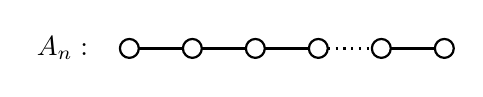
\begin{tikzpicture}[scale=.4]
\draw (-1,0) node[anchor=east]  {$A_n:$};
\foreach \x in {0,...,5}
\draw[xshift=\x cm, thick] (\x cm,0) circle (.3cm);
\draw[thick] (0.3 cm, 0) -- +(1.4 cm, 0);
\draw[thick] (2.3 cm, 0) -- +(1.4 cm, 0);
\draw[thick] (4.3 cm, 0) -- +(1.4 cm, 0);
\draw[dotted, thick] (6.3 cm, 0) -- +(1.4 cm, 0);
\draw[thick] (8.3 cm, 0) -- +(1.4 cm, 0);
\end{tikzpicture}

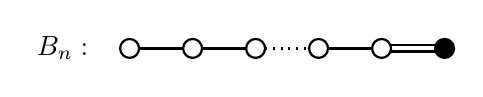
\begin{tikzpicture}[scale=.4]
\draw (-1,0) node[anchor=east]  {$B_n:$};
\foreach \x in {0,...,4}
\draw[xshift=\x cm, thick] (\x cm,0) circle (.3cm);
\draw[xshift=5 cm, thick, fill=black] (5 cm,0) circle (.3cm);
\draw[thick] (0.3 cm, 0) -- +(1.4 cm, 0);
\draw[thick] (2.3 cm, 0) -- +(1.4 cm, 0);
\draw[dotted,thick] (4.3 cm, 0) -- +(1.4 cm, 0);
\draw[thick] (6.3 cm, 0) -- +(1.4 cm, 0);
\draw[thick] (8.3 cm, 0.1) -- +(1.4 cm, 0);
\draw[thick] (8.3 cm, -0.1) -- +(1.4 cm, 0);
\end{tikzpicture}

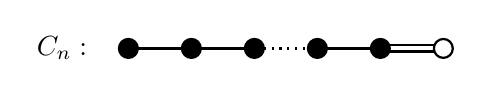
\begin{tikzpicture}[scale=.4]
\draw (-1,0) node[anchor=east]  {$C_n:$};
\foreach \x in {0,...,4}
\draw[xshift=\x cm, thick, fill=black] (\x cm,0) circle (.3cm);
\draw[xshift=5 cm, thick] (5 cm,0) circle (.3cm);
\draw[thick] (0.3 cm, 0) -- +(1.4 cm, 0);
\draw[thick] (2.3 cm, 0) -- +(1.4 cm, 0);
\draw[dotted,thick] (4.3 cm, 0) -- +(1.4 cm, 0);
\draw[thick] (6.3 cm, 0) -- +(1.4 cm, 0);
\draw[thick] (8.3 cm, 0.1) -- +(1.4 cm, 0);
\draw[thick] (8.3 cm, -0.1) -- +(1.4 cm, 0);
\end{tikzpicture}

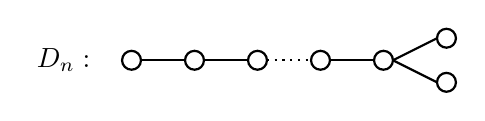
\begin{tikzpicture}[scale=.4]
\draw (-1,0) node[anchor=east]  {$D_n:$};
\foreach \x in {0,...,4}
\draw[xshift=\x cm, thick] (\x cm,0) circle (.3cm);
\draw[xshift=5 cm, thick] (5 cm, .7) circle (.3cm);
\draw[xshift=5 cm, thick] (5 cm, -.7) circle (.3cm);
\draw[thick] (0.3 cm, 0) -- +(1.4 cm, 0);
\draw[thick] (2.3 cm, 0) -- +(1.4 cm, 0);
\draw[dotted,thick] (4.3 cm, 0) -- +(1.4 cm, 0);
\draw[thick] (6.3 cm, 0) -- +(1.4 cm, 0);
\draw[thick] (8.3 cm, 0) -- +(1.4 cm, .7);
\draw[thick] (8.3 cm, 0) -- +(1.4 cm, -.7);
\end{tikzpicture}

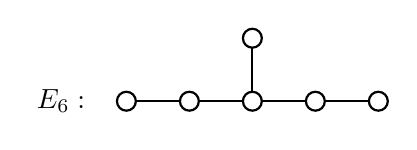
\begin{tikzpicture}[scale=.4]
\draw (-1,0) node[anchor=east]  {$E_6:$};
\foreach \x in {0,...,4}
\draw[thick,xshift=\x cm] (\x cm,0) circle (3 mm);
\foreach \y in {0,...,3}
\draw[thick,xshift=\y cm] (\y cm,0) ++(.3 cm, 0) -- +(14 mm,0);
\draw[thick] (4 cm, 2 cm) circle (3 mm);
\draw[thick] (4 cm, 3mm) -- +(0, 1.4 cm);
\end{tikzpicture}

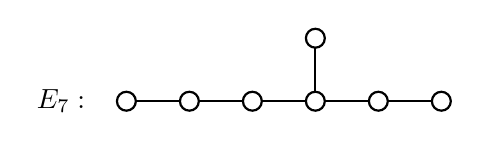
\begin{tikzpicture}[scale=.4]
\draw (-1,0) node[anchor=east]  {$E_7:$};
\foreach \x in {0,...,5}
\draw[thick,xshift=\x cm] (\x cm,0) circle (3 mm);
\foreach \y in {0,...,4}
\draw[thick,xshift=\y cm] (\y cm,0) ++(.3 cm, 0) -- +(14 mm,0);
\draw[thick] (6 cm,2 cm) circle (3 mm);
\draw[thick] (6 cm, 3mm) -- +(0, 1.4 cm);
\end{tikzpicture}

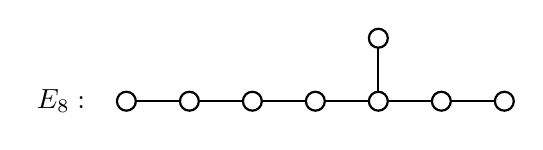
\begin{tikzpicture}[scale=.4]
\draw (-1,0) node[anchor=east]  {$E_8:$};
\foreach \x in {0,...,6}
\draw[thick,xshift=\x cm] (\x cm,0) circle (3 mm);
\foreach \y in {0,...,5}
\draw[thick,xshift=\y cm] (\y cm,0) ++(.3 cm, 0) -- +(14 mm,0);
\draw[thick] (8 cm,2 cm) circle (3 mm);
\draw[thick] (8 cm, 3mm) -- +(0, 1.4 cm);
\end{tikzpicture}

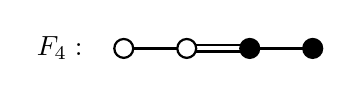
\begin{tikzpicture}[scale=.4]
\draw (-1,0) node[anchor=east] {$F_4:$};
\foreach \x in {0,...,1}
\draw[thick, xshift=\x cm] (\x cm, 0) circle (3 mm);
\foreach \x in {2,...,3}
\draw[thick, xshift=\x cm, fill=black] (\x cm, 0) circle (3 mm);
\draw[thick] (0.3 cm, 0) -- +(1.4 cm, 0);
\draw[thick] (2.3 cm, 0.1) -- +(1.4 cm, 0);
\draw[thick] (2.3 cm, -0.1) -- +(1.4 cm, 0);
\draw[thick] (4.3 cm, 0) -- +(1.4 cm, 0);
\end{tikzpicture}

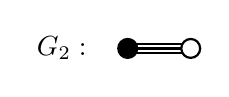
\begin{tikzpicture}[scale=.4]
\draw (-1,0) node[anchor=east]  {$G_2:$};
\draw[thick, fill=black] (0 ,0) circle (.3 cm);
\draw[thick] (2 cm,0) circle (.3 cm);
\draw[thick] (30: 3mm) -- +(1.5 cm, 0);
\draw[thick] (0: 3 mm) -- +(1.4 cm, 0);
\draw[thick] (-30: 3 mm) -- +(1.5 cm, 0);
\end{tikzpicture}

\section{Cartan Matrix}\label{cartan}

The matrix of Cartan integers for root systems of rank 2, defined by
\begin{align*}
\left(\begin{matrix}\langle \alpha, \alpha\rangle & \langle \alpha, \beta \rangle \\ \langle \beta, \alpha \rangle & \langle \beta, \beta \rangle\end{matrix}\right).
\end{align*}
If the roots are of different length then $\alpha$ is the shorter root.

\begin{align*}
	A_1\times A_1:&\left(\begin{array}{rr}2 & 0\\0 & 2\end{array}\right) &B_2:&\left(\begin{array}{rr}2 & -1\\-2 & 2\end{array}\right) \\
	A_2:&\left(\begin{array}{rr}2 & -1\\-1 & 2\end{array}\right) &G_2:&\left(\begin{array}{rr}2 & -1\\-3 & 2\end{array}\right).
\end{align*}

\section{Rank 2 Root System Diagrams}\label{rank2diagrams}

$A_1\times A_1:$
\begin{center}
\begin{tikzpicture}[>=latex, scale=1.2]
\pgfmathsetmacro\ax{2}
\pgfmathsetmacro\ay{0}
\pgfmathsetmacro\bx{0}
\pgfmathsetmacro\by{2}
\draw[red,->] (0,0) -- (\ax,\ay) node[right] {\(\alpha\)};
\draw[red,->] (0,0) -- (\bx,\by) node[above] {\(\beta\)};
\draw[->] (0,0) -- (-\ax,-\ay) node[left] {\(-\alpha\)};
\draw[->] (0,0) -- (-\bx,-\by) node[below] {\(-\beta\)};
\end{tikzpicture}
\end{center}

$A_2:$ 
\begin{center}
\begin{tikzpicture}[>=latex, scale=1.2]
\pgfmathsetmacro\ax{2}
\pgfmathsetmacro\ay{0}
\pgfmathsetmacro\bx{2 * cos(120)}
\pgfmathsetmacro\by{2 * sin(120)}
\draw[red,->] (0,0) -- (\ax,\ay) node[right] {\(\alpha\)};
\draw[red,->] (0,0) -- (\bx,\by) node[above left] {\(\beta\)};
\draw[->] (0,0) -- (-\ax,-\ay) node[left] {\(-\alpha\)};
\draw[->] (0,0) -- (-\bx,-\by) node[below right] {\(-\beta\)};
\draw[->] (0,0) -- (\ax + \bx,\ay + \by) node[above right] {\(\alpha+\beta\)};
\draw[->] (0,0) -- (-\ax - \bx,-\ay - \by) node[below left] {\(-\alpha-\beta\)};
\end{tikzpicture}
\end{center}

$B_2:$
\begin{center}
\begin{tikzpicture}[>=latex, scale=1.2]
\pgfmathsetmacro\ax{2}
\pgfmathsetmacro\ay{0}
\pgfmathsetmacro\bx{-2}
\pgfmathsetmacro\by{2}
\draw[red,->] (0,0) -- (\ax,\ay) node[right] {\(\alpha\)};
\draw[red,->] (0,0) -- (\bx,\by) node[above left] {\(\beta\)};
\draw[->] (0,0) -- (-\ax,-\ay) node[left] {\(-\alpha\)};
\draw[->] (0,0) -- (-\bx,-\by) node[below right] {\(-\beta\)};
\draw[->] (0,0) -- (\ax + \bx,\ay + \by) node[above] {\(\alpha+\beta\)};
\draw[->] (0,0) -- (-\ax - \bx,-\ay - \by) node[below] {\(-\alpha-\beta\)};
\draw[->] (0,0) -- (2*\ax + \bx,2*\ay + \by) node[above right] {\(2\alpha+\beta\)};
\draw[->] (0,0) -- (-2*\ax - \bx,-2*\ay - \by) node[below left] {\(-2\alpha-\beta\)};
\end{tikzpicture}
\end{center}

$G_2:$ 
\begin{center}
\begin{tikzpicture}[>=latex, scale=1.2]
\pgfmathsetmacro\ax{2}
\pgfmathsetmacro\ay{0}
\pgfmathsetmacro\abx{2 * cos(120)}
\pgfmathsetmacro\aby{2 * sin(120)}
\draw[red,->] (0,0) -- (\ax,\ay) node[below right] {\(\alpha\)};
\draw[red,->] (0,0) -- (-\ax + \abx,-\ay + \aby) node[above] {\(\beta\)};
\draw[->] (0,0) -- (-\ax,-\ay) node[below left] {\(-\alpha\)};
\draw[->] (0,0) -- (\ax - \abx,\ay - \aby) node[below] {\(-\beta\)};
\draw[->] (0,0) -- (\abx,\aby) node[above] {\(\alpha+\beta\)};
\draw[->] (0,0) -- (-\abx,-\aby) node[below] {\(-\alpha-\beta\)};
\draw[->] (0,0) -- (\ax + \abx,\ay + \aby) node[above] {\(2\alpha+\beta\)};
\draw[->] (0,0) -- (-\ax-\abx,-\ay-\aby) node[below] {\(-2\alpha-\beta\)};
\draw[->] (0,0) -- (2*\ax + \abx,2*\ay + \aby) node[above] {\(3\alpha+\beta\)};
\draw[->] (0,0) -- (-2*\ax - \abx,-2*\ay - \aby) node[below] {\(-3\alpha-\beta\)};
\draw[->] (0,0) -- (\ax + 2*\abx,\ay + 2*\aby) node[above] {\(3\alpha+2\beta\)};
\draw[->] (0,0) -- (-\ax - 2*\abx,-\ay - 2*\aby) node[below] {\(-3\alpha-2\beta\)};
\end{tikzpicture}
\end{center}
        % Source Code

%%!TEX root = /Users/dan/Documents/Thesis/Thesis.tex
% Appendix C

\chapter{Rank 2 Root System Diagrams}
\label{AppendixC}
\lhead{Appendix C. \emph{Rank 2 Root System Diagrams}}

\begin{center}
	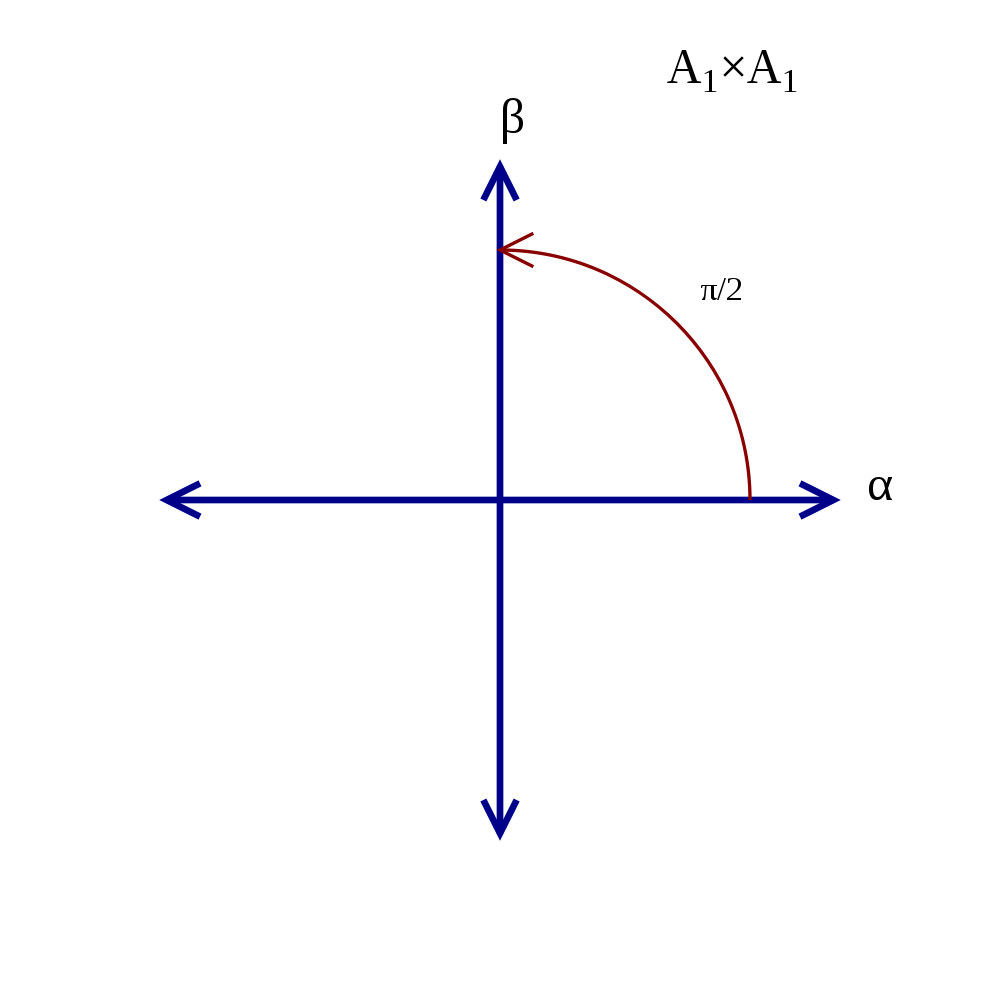
\includegraphics[scale=0.33]{a1a1.png}
\end{center}

\begin{center}
	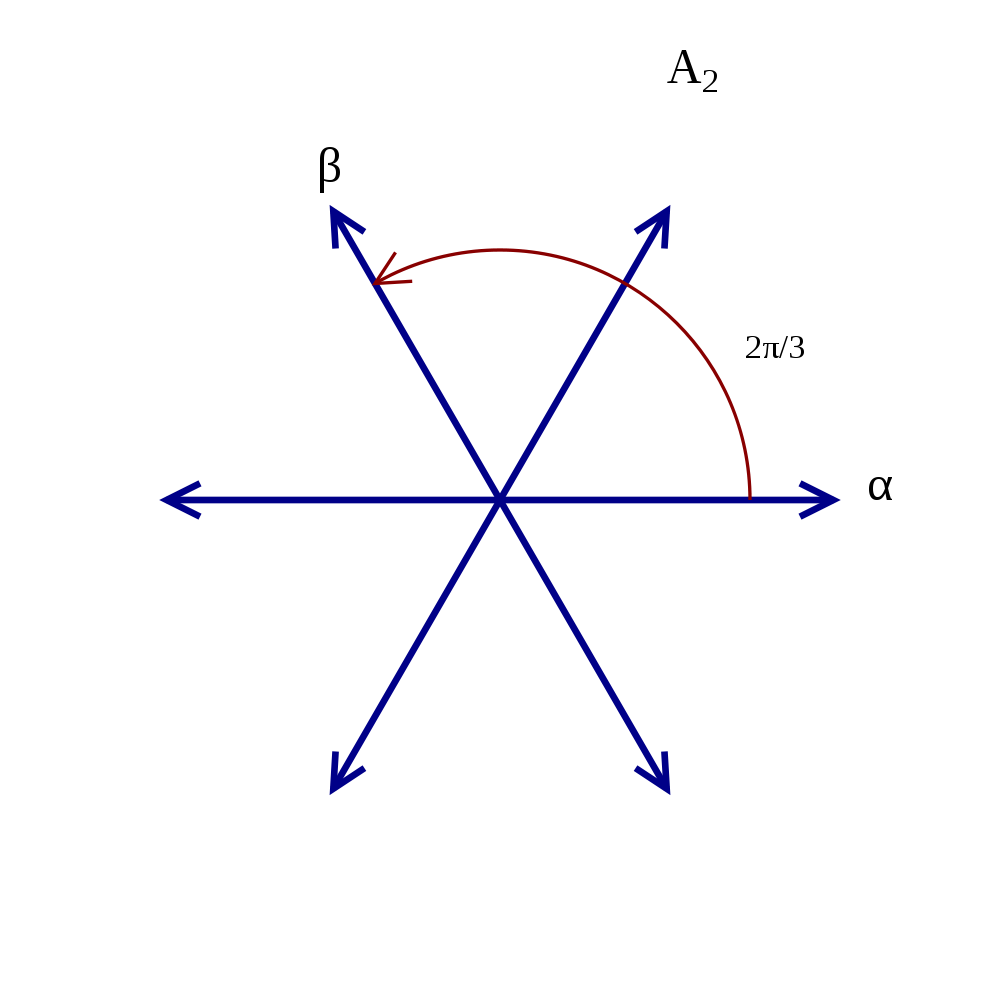
\includegraphics[scale=0.33]{a2.png}
\end{center}

\begin{center}
	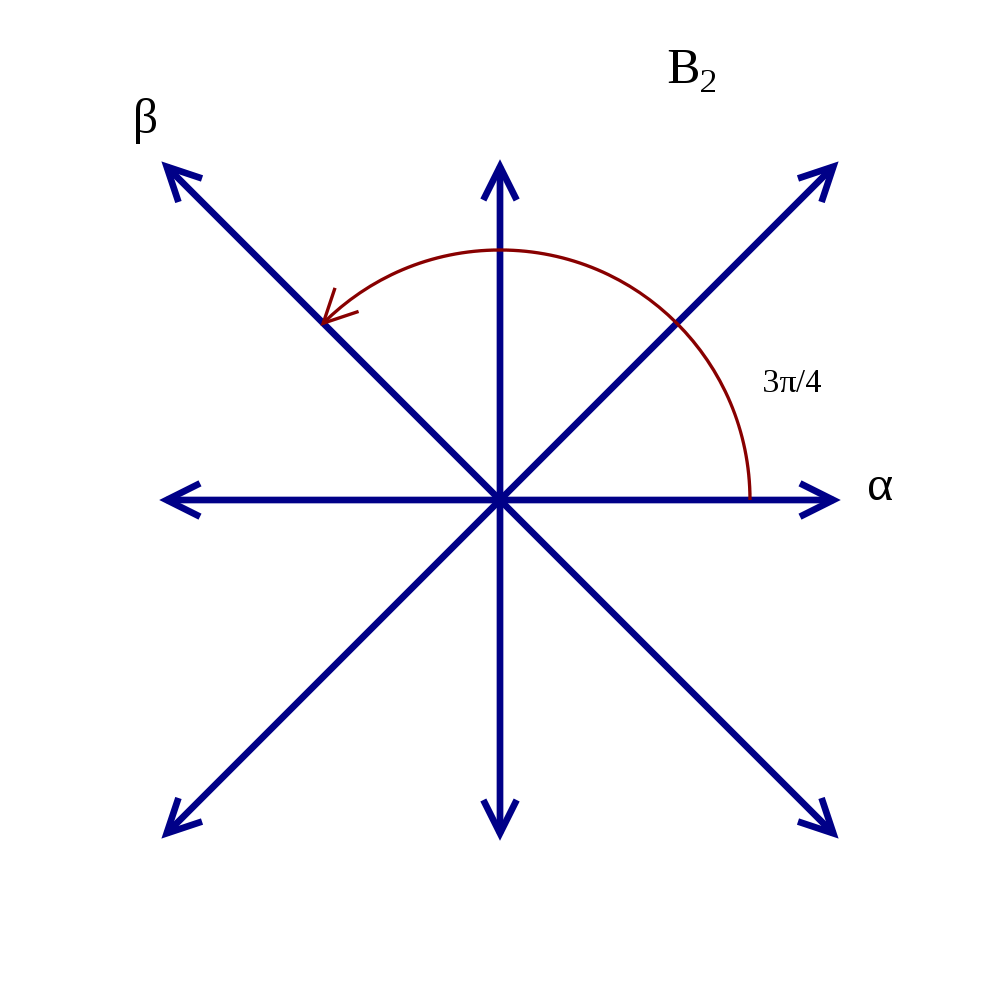
\includegraphics[scale=0.33]{b2.png}
\end{center}

\begin{center}
	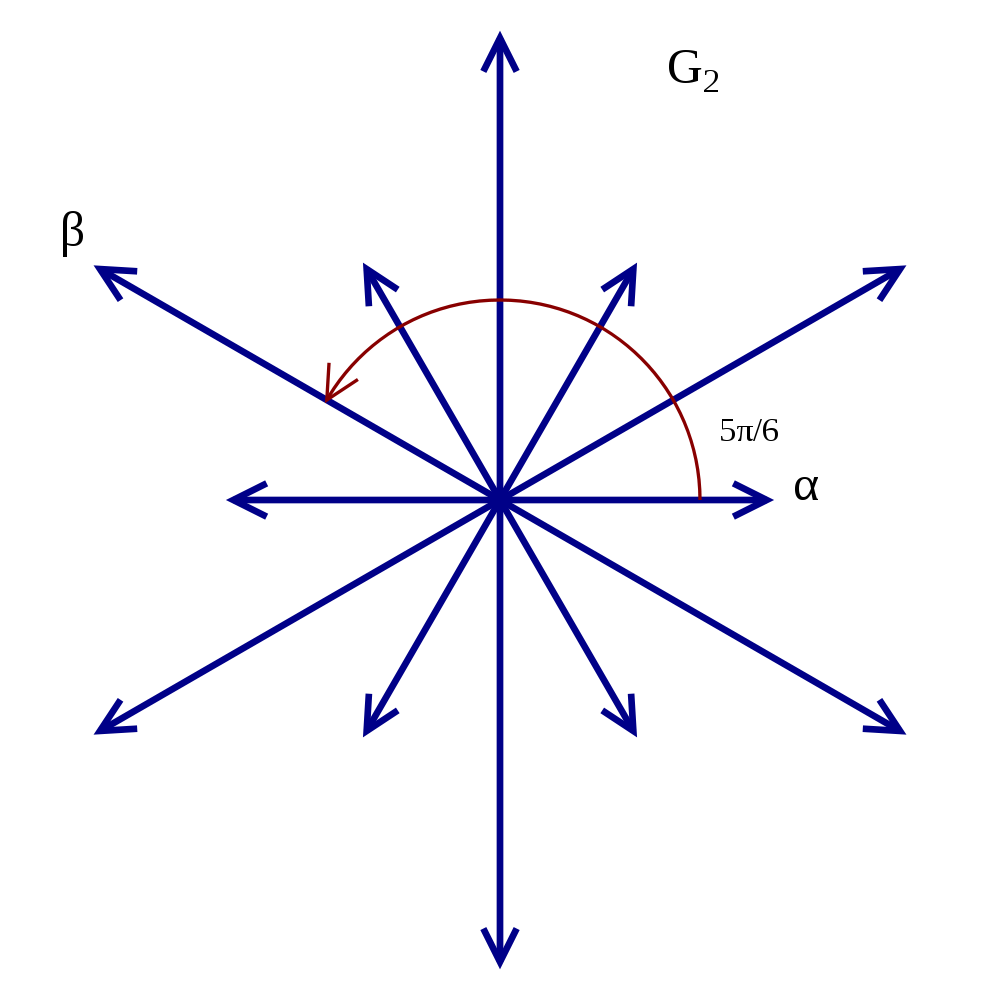
\includegraphics[scale=0.33]{g2.png}
\end{center}
 % Appendix Title

\addtocontents{toc}{\vspace{2em}}  % Add a gap in the Contents, for aesthetics
\backmatter

%% ----------------------------------------------------------------
\label{Bibliography}
\lhead{\emph{Bibliography}}  % Change the left side page header to "Bibliography"
\bibliographystyle{unsrtnat}  % Use the "unsrtnat" BibTeX style for formatting the Bibliography
\bibliography{Bibliography}  % The references (bibliography) information are stored in the file named "Bibliography.bib"

\end{document}  % The End
%% ----------------------------------------------------------------